\documentclass{scalatekids-article}
\usepackage[italian]{babel}
\begin{document}
\lfoot{Analisi dei Requisiti 4.0.0}
\newgeometry{top=3.5cm}
\begin{titlepage}
  \begin{center}
    \begin{center}
      
\includegraphics[width=10cm]{sklogo.png}
    \end{center}
    \vspace{1cm}
    \begin{Huge}
      \begin{center}
        \textbf{Analisi dei Requisiti}
      \end{center}
    \end{Huge}
    \vspace{11pt}
    \bgroup
    \def\arraystretch{1.3}
    \begin{tabular}{r|l}
      \multicolumn{2}{c}{\textbf{Informazioni sul documento}} \\
      \hline
      \setbox0=\hbox{0.0.1\unskip}\ifdim\wd0=0pt
      \\
      \else
      \textbf{Versione} & 4.0.0\\
      \fi
      \textbf{Redazione} & \multiLineCell[t]{Marco Boseggia\\Francesco Agostini\\Giacomo Vanin}\\
      \textbf{Verifica} & \multiLineCell[t]{Michael Munaro\\Marco Boseggia}\\
      \textbf{Approvazione} & \multiLineCell[t]{Davide Trevisan}\\
      \textbf{Uso} & Esterno\\
      \textbf{Lista di Distribuzione} & \multiLineCell[t]{ScalateKids\\Prof. Tullio Vardanega\\Prof. Riccardo Cardin}\\
    \end{tabular}
    \egroup
    \vspace{22pt}
  \end{center}
\end{titlepage}
\restoregeometry{}
\clearpage
\pagenumbering{Roman}
\setcounter{page}{1}
\begin{flushleft}
  \vspace{0cm}
  {\large\bfseries Diario delle modifiche \par}
\end{flushleft}
\vspace{0cm}
\begin{center}
  \begin{longtable}{| l | l | l | l | p{5cm} |}
    \hline
    Versione & Autore & Ruolo & Data & Descrizione \\
    \hline
    4.0.0 & Davide Trevisan & Responsabile & 2016-06-15 & Approvazione documento\\
    \hline
    3.2.0 & Michael Munaro & Verificatore & 2016-06-07 & Verifica Incrementi\\
    \hline
    3.1.3 & Marco Boseggia & Analista & 2016-06-06 & Aggiornamento tracciamento\\
    \hline
    3.1.2 & Francesco Agostini & Analista & 2016-06-03 & Aggiornamento requisiti\\
    \hline
    3.1.1 & Giacomo Vanin & Analista & 2016-06-01 & Aggiornamento vincoli password nelle sezioni 3.45, 3.46\\
    \hline
    3.1.0 & Marco Boseggia & Verificatore & 2016-05-27 & Verifica modifiche apportate\\
    \hline
    3.0.1 & Alberto De Agostini & Analista & 2016-05-27 & Apportate modifiche post RP (immagine in sezione 3.50 e numeramento sezione 4)\\
    \hline
    3.0.0 & Francesco Agostini & Responsabile & 2016-05-04 & Approvazione documento\\
    \hline
    2.2.0 & Marco Boseggia & Verificatore & 2016-04-28 & Verifica aggiornamento requisiti \\
    \hline
    2.1.1 & Francesco Agostini & Analista & 2016-04-26 & Aggiornamento requisiti \\
    \hline
    2.1.0 & Alberto De Agostini & Verificatore & 2016-04-28 & Verifica incrementi \\
    \hline
    2.0.2 & Andrea Baldan & Analista & 2016-04-27 & Aggiornamento requisiti minimi sezione 2.4 \\
    \hline
    2.0.1 & Andrea Baldan & Analista & 2016-04-26 & Aggiornamento requisiti \\
    \hline
    2.0.0 & Giacomo Vanin & Responsabile & 2016-04-09 & Approvazione documento\\
    \hline
    1.6.0 & Marco Boseggia & Verificatore & 2016-04-05 & Verifica sezione tracciamento requisiti-test\\
    \hline
    1.5.1 & Alberto De Agostini & Analista & 2016-04-05 & Stesura sezione Tracciamento requisiti-test\\
    \hline
    1.5.0 & Andrea Giacomo Baldan & Verificatore & 2016-03-13 & Verifica sezioni tracciamento requisiti-fonti e tracciamento fonti-requisiti\\
    \hline
    1.4.1 & Francesco Agostini & Analista & 2016-03-11 & Stesura sezioni Tracciamento requisiti fonti e tracciamento fonti requisiti\\
    \hline
    1.4.0 & Marco Boseggia & Verificatore & 2016-03-10 & Verifica sezione requisiti\\
    \hline
    1.3.1 & Andrea Giacomo Baldan & Analista & 2016-03-09 & Stesura sezione requisiti\\
    \hline
    1.3.0 & Andrea Giacomo Baldan & Verificatore & 2016-03-05 & verifica sezione Casi d'uso\\
    \hline
    1.2.3 & Michael Munaro & Analista & 2016-03-04 & Modifica casi d'uso da UC2.4 a UC2.13 e sottocasi d'uso\\
    \hline
    1.2.2 & Alberto De Agostini & Analista & 2016-03-01 & Modifica casi d'uso UC2, 2.1, 2.2, 2.3 e sottocasi d'uso\\
    \hline
    1.2.1 & Francesco Agostini & Analista & 2016-02-28 & Modifica casi d'uso UC1.9, 1.10, 1.11, 1.12, 1.13, 1.14, 1.15 e sottocasi d'uso\\
    \hline
    1.2.0 & Michael Munaro & Verificatore & 2016-02-27 & Verifica sezione Casi d'uso\\
    \hline
    1.1.2 & Michael Munaro & Analista & 2016-02-26 & Modifica casi d'uso UC1.5, 1.6, 1.7, 1.8 e sottocasi d'uso\\
    \hline
    1.1.1 & Andrea Giacomo Baldan & Analista & 2016-02-25 & Modifica casi d'uso UC1, 1.1, 1.2, 1.3, 1.4 e sottocasi d'uso\\
    \hline
    1.1.0 & Marco Boseggia & Verificatore & 2016-02-23 & Verifica sezione 3.2\\
    \hline
    1.0.1 & Francesco Agostini & Analista & 2016-02-22 & Stesura sezione 3.2\\
    \hline
    1.0.0 & Andrea Giacomo Baldan & Responsabile & 2016-01-20 & Approvazione documento\\
    \hline
    0.4.0 & Giacomo Vanin & Verificatore & 2016-01-19 & Verifica sezione Tracciamento\\
    \hline
    0.3.1 & Marco Boseggia & Analista & 2016-01-18 & Stesura sezione Tracciamento\\
    \hline
    0.3.0 & Alberto De Agostini & Verificatore & 2016-01-16 & Verifica sezione Classificazione Requisiti\\
    \hline
    0.2.3 & Michael Munaro & Analista & 2016-01-15 & Integrazione sezione Classificazione Requisiti\\
    \hline
    0.2.1 & Marco Boseggia & Analista & 2016-01-14 & Stesura sezione Classificazione Requisiti\\
    \hline
    0.2.2 & Davide Trevisan & Analista & 2016-01-14 & Correzione sezione Casi d'uso\\
    \hline
    0.2.0 & Giacomo Vanin & Verificatore & 2016-01-12 & Verifica sezione Casi d'uso\\
    \hline
    0.1.1 & Michael Munaro & Analista & 2016-01-10 & Integrazione sezione Casi d'uso\\
    \hline
    0.1.0 & Alberto De Agostini & Verificatore & 2016-01-07 & Verifica sezioni stese in precedenza\\
    \hline
    0.0.4 & Davide Trevisan & Analista & 2016-01-05 & Integrazione sezione Casi d'uso\\
    \hline
    0.0.3 & Marco Boseggia & Analista & 2016-01-04 & Inizio stesura sezione Casi d'uso\\
    \hline
    0.0.2 & Michael Munaro & Analista & 2016-01-03 & Stesura sezione Descrizione Generale\\
    \hline
    0.0.1 & Andrea Giacomo Baldan & Amministratore & 2015-12-16 & Creazione scheletro del documento\\
    \hline
  \end{longtable}
\end{center}
\tableofcontents
\newpage
\pagenumbering{arabic}

\section{Sommario}

\subsection{Scopo del documento}

Il seguente documento ha lo scopo di presentare le funzionalità che il prodotto
\textbf{Actorbase} esporrà all'utilizzatore finale. Inoltre elenca e descrive i
requisiti derivanti dalle suddette funzionalità, emersi durante le riunioni
interne ed esterne con il \textit{Proponente}.
\prodPurpose{}\glossExpl{}

\subsection{Riferimenti}

\subsubsection{Normativi}

\begin{itemize}
\item\textbf{Capitolato d'appalto C1:} \textit{Actorbase: a NoSQL DB based on the Actor model}\\
  \url{http://www.math.unipd.it/~tullio/IS-1/2015/Progetto/C1.pdf}
\item\textbf{Verbale esterno:}\\
  \href{run:../RR/Interni/VerbaleEsterno20160112\_v1.0.0.pdf}{Verbale Esterno 20160112 v1.0.0}\\
  \href{run:../RR/Interni/VerbaleEsterno20160119\_v1.0.0.pdf}{Verbale Esterno 20160119 v1.0.0}
\item\textbf{Norme di Progetto:}\\
  \href{run:../Interni/NormeDiProgetto\_v4.0.0.pdf}{Norme di Progetto v4.0.0}
\end{itemize}

\subsubsection{Informativi}

\begin{itemize}
\item\textbf{Dispense fornite dall'insegnamento Ingegneria del Software mod. A:}\\
  \url{http://www.math.unipd.it/~tullio/IS-1/2015/Dispense/L06.pdf}
\item\textbf{Dispense fornite dall'insegnamento Ingegneria del Software mod. A:}\\
  \url{http://www.math.unipd.it/~tullio/IS-1/2015/Dispense/E02.pdf}
\item\textbf{CAP theorem:}\\
  \url{https://en.wikipedia.org/wiki/CAP_theorem}
\item\textbf{Reactive Manifesto:}\\
  \url{http://www.reactivemanifesto.org/}\\
  \url{https://en.wikipedia.org/wiki/Reactive_programming}
\item\textbf{Amazon DynamoDB:}\\
  \url{http://docs.aws.amazon.com/amazondynamodb/latest/developerguide/Introduction.html}
\item\textbf{Leader election:}\\
  \url{https://en.wikipedia.org/wiki/Leader_election}
\end{itemize}

\section{Descrizione generale}

\subsection{Prospettive del prodotto}

l'obiettivo del prodotto è fornire un \gloss{database} \gloss{NoSQL} di tipo
\gloss{key-value}, quindi senza schemi predefiniti e tabelle; che utilizzi il
modello ad \gloss{attori} per garantire un alto grado di \gloss{concorrenza} e
\gloss{scalabilità orizzontale} idealmente illimitata.

\subsection{Funzioni}

Il software fornirà un sistema di interazione con l'utente basata su \gloss{UI}
testuale direttamente da riga di comando. Questa permetterà di effettuare le operazioni
basilari che ogni \gloss{database} fornisce:
\begin{itemize}
\item Creazione di una o più \gloss{collezioni};
\item Cancellazione di una o più \gloss{collezioni};
\item Modifica del nome di una \gloss{collezione};
\item Ricerca all'interno del \gloss{database} o all'interno di una o più \gloss{collezioni};
\item Inserimento \gloss{item} con o senza sovrascrittura;
\item Cancellazione \gloss{item};
\item Connessione ad altre istanze \textbf{Actorbase}.
\end{itemize}
Il programma inoltre permetterà la richiesta di un aiuto esplicativo sull'uso
dei comandi.

\subsection{Caratteristiche utenza}

Il prodotto è orientato all'utilizzo da parte di clientela interessata a
sviluppo di applicazioni \gloss{reactive}, che trattino grandi moli di dati e
debbano fornire brevissimi tempi di risposta sacrificando dunque le funzionalità
relazionali tipiche dei tradizionali \gloss{database} \textit{SQL} in favore di
un sistema fortemente \gloss{concorrente} e senza l'\gloss{overhead} generato
dagli schemi \gloss{SQL}.

\subsection{Vincoli}
% TODO mettere nuovi requisiti minimi...
Per far funzionare \textbf{Actorbase} sarà necessario disporre di un computer con
installata la \textit{\gloss{JVM} versione 8}. I sistemi operativi supportati sono:
\begin{itemize}
\item Ubuntu 14.04 LTS o successivo;
\item Windows 10;
\item Mac OSX El Capitan o successivo.
\end{itemize}
I requisiti minimi per Java 8 sono:
\begin{itemize}
\item RAM:\@128 MB;\@
\item Spazio su disco: 124MB;\@
\item Processore: minimo Pentium 2 a 266 MHz;
\end{itemize}
I requisiti minimi consigliati per la componente server del sistema \textbf{Actorbase} sono:
\begin{itemize}
\item RAM:\@4 GB;\@
\item Spazio su disco: 1 GB;\@
\item Processore: x64 a 1.2GHz;
\end{itemize}
I requisiti minimi consigliati per la componente client del sistema \textbf{Actorbase} sono:
\begin{itemize}
\item RAM:\@1 GB;\@
\item Spazio su disco: 512MB;\@
\item Processore: x64 a 1.2GHz;
\end{itemize}
Questi requisiti potrebbero aumentare in base all'utilizzo che si vuole fare del software.
In particolare la quantità di RAM e di spazio su disco potrebbe variare in base al carico
di dati su server.

\section{Casi d'uso}

Le aspettative di esperienza utente derivano dall'utilizzo da parte dei
componenti del gruppo di \gloss{Amazon DynamoDB}, un \gloss{database}
\gloss{key-value} sviluppato da \textit{Amazon}, utilizzato come modello di
riferimento per lo sviluppo. I casi d'uso seguono le norme di stesura elencate
nel documento \href{run:../Interni/NormeDiProgetto\_v4.0.0.pdf}{Norme di
  Progetto v4.0.0}.

\subsection{Identificazione attori}

L'analisi del capitolato e le riunioni con il \textit{Proponente} hanno fatto emergere alcune considerazioni sull'obiettivo che \textbf{Actorbase} si pone di raggiungere.\\Trattandosi di un'applicazione distribuita il prodotto finale sarà costituito da due \gloss{macro} componenti: un lato server e un lato client fornito di interfaccia comandi testuale per poter dialogare con la base di dati.\\ Suddivisione attori:\\
\textbf{Primari}
\begin{itemize}
\item\textbf{Utente non autenticato:}\\
  Rappresenta l'utente generico che avvia la \gloss{CLI} (Command Line Interface) di \textbf{Actorbase} ma non è ancora connesso al lato server del prodotto;
\item\textbf{Utente autenticato:}\\
  Rappresenta l'utente generico connesso al lato server del prodotto;
\item\textbf{Amministratore:}\\
  Rappresenta un superutente con privilegi di lettura e scrittura su tutte le \gloss{collezioni} presenti all'interno del database;
\item\textbf{Programma esterno su JVM:}\\
  Nel caso di utilizzo del sistema da un programma esterno su \gloss{JVM}, sarà quest'ultimo ad essere attore primario rispetto al \gloss{driver} da utilizzare per
  interfacciarsi con il sistema \textbf{Actorbase}. Il sistema \textbf{Actorbase} sarà considerato un attore secondario del \gloss{driver}, in quanto serve allo scopo
  per raggiungere l'obiettivo richiesto dall'attore primario, ovvero l'inserimento dei comandi al sistema.
\end{itemize}
\textbf{Secondari}
\begin{itemize}
\item\textbf{Actorbase:}\\
  Nel caso di utilizzo del sistema da un programma esterno in linguaggio Scala, il sistema \textbf{Actorbase} rappresenta effettivamente l'attore necessario agli attori primari per raggiungere
  lo scopo prefissato, ovvero l'inserimento dei comandi da inviare al sistema stesso mediante utilizzo del \gloss{driver}.
\end{itemize}

\subsubsection{Permessi}
\label{sec:permessi}

Si è scelto di utilizzare il classico sistema di permessi, ovvero lettura e scrittura. Perciò ogni utente ha permessi di lettura e scrittura sulle proprie \gloss{collezioni}. Se un utente invece decide di aggiungere un collaboratore ad una propria \gloss{collezione}, esso può scegliere se garantire accesso in sola lettura o se dare pieni permessi di lettura e scrittura al collaboratore designato.\\L'utente amministratore essendo tale ha permessi di lettura e scrittura sull'intero database.\\

% *vecchio paragrafo della visibilità* Rispetto al classico sistema di permessi di lettura e scrittura, \textbf{Actorbase}
% prevede un meccanismo semplificato di \gloss{visibilità} secondo le seguenti regole:
% \begin{itemize}
% \item Ogni utente autenticato inizialmente ha \gloss{visibilità} solo sulle proprie \gloss{collezioni} e/o su \gloss{collezioni} di proprietà altrui su cui è in collaborazione;
% \item L'utente amministratore ha \gloss{visibilità} su tutto il sistema \textbf{Actorbase}.
% \end{itemize}
% La \gloss{visibilità} garantisce privilegi sia in lettura che in scrittura. Di
% conseguenza tutte le azioni descritte nei casi d'uso si applicano al livello di
% \gloss{visibilità} proprio dell'attore che le effettua.

\subsubsection{Scalabilità orizzontale}

Il vantaggio più grande che il prodotto dovrà offrire sarà la possibilità di
\gloss{scale out} semplificata al massimo. Dovrà quindi essere possibile
aggiungere potenza di calcolo e capacità di carico mediante affiancamento di
macchine aggiuntive. I dati contenuti all'interno della base di dati originaria
dovranno essere redistribuiti e bilanciati tra i nuovi nodi inseriti. In questo
modo è idealmente possibile ottenere infinita capacità di carico semplicemente
aggiungendo risorse hardware qualora necessario.

\subsection{Visione generale}

L'immagine che segue rappresenta uno schema della visione d'insieme del
funzionamento di Actorbase. Al suo interno è possibile identificare l'utente
che, mediante CLI e accesso alla rete, è in grado di interagire con la rete
Actorbase. Essa è formata da un sistema di database distribuiti la cui
distribuzione è assolutamente trasparente all'utente. Ogni elemento del sistema
è in comunicazione con tutte le altre istanze con cui è in grado di interagire
in maniera autonoma.
\begin{figure}[H]
  \begin{center}
    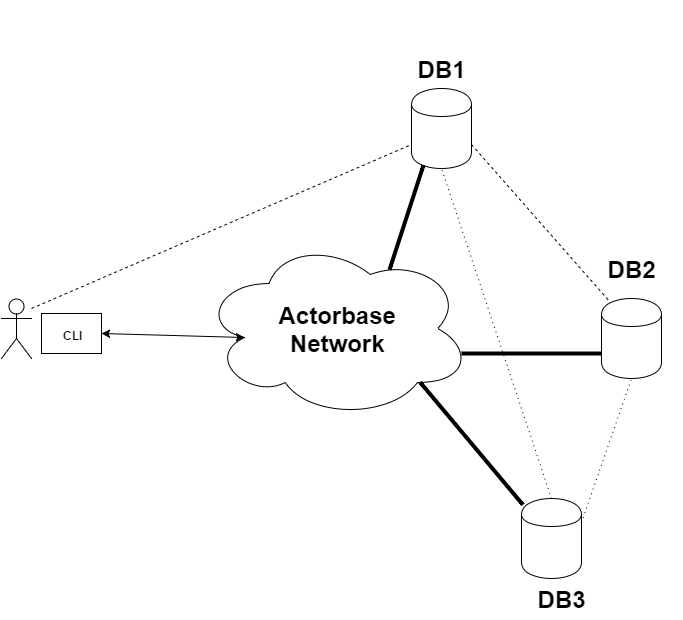
\includegraphics[width=0.7\textwidth,keepaspectratio]{UseCases/ActorbaseNetwork.png}
    \caption{Actorbase: Visione generale semplificata rete Actorbase}
  \end{center}
\end{figure}

\subsection{UC1: Interazioni tramite CLI}

\begin{figure}[H]
  \begin{center}
    \includegraphics[width=0.6\textwidth,keepaspectratio]{UseCases/UC1.png}
    \caption{Caso d'uso 1: Interazioni tramite CLI}
  \end{center}
\end{figure}
\textbf{Attori primari:} utente non autenticato, utente autenticato, utente amministratore\\
\textbf{Scopo e descrizione:} L'attore ha appena avviato la \gloss{CLI}, le operazioni che può eseguire sono:
\begin{itemize}
\item Nel caso sia un \textbf{utente non autenticato}:
  \begin{itemize}
  \item Effettuare il login;
  \item Richiedere aiuto a livello generale o a livello di comando.
  \end{itemize}
\item Nel caso sia un \textbf{utente autenticato} o un \textbf{utente amministratore}:
  \begin{itemize}
  \item Richiedere aiuto a livello generale o a livello di comando;
  \item Effettuare operazioni sulle \gloss{collezioni};
  \item Effettuare operazioni sugli \gloss{item};
  \item Effettuare una ricerca su una o più \gloss{collezioni};
  \item Modificare la propria password;
  \item Effettuare il logout.
  \end{itemize}
\item Nel caso sia un \textbf{utente amministratore}:
  \begin{itemize}
  \item Effettuare operazioni di gestione utenti.
  \end{itemize}
\end{itemize}
\textbf{Precondizione:} il server è in ascolto\\
\textbf{Scenario principale:} le operazioni sono possibili da diversi tipi di attore come si può vedere dal diagramma Caso d'uso 1.
\begin{itemize}
\item UC1.1\ -\ Login;
\item UC1.2\ -\ Richiesta aiuto.
  \begin{itemize}
  \item UC1.2.1\ -\ Aiuto generale;
  \item UC1.2.2\ -\ Aiuto comando.
  \end{itemize}
\end{itemize}
% \textbf{Scenario principale utente autenticato o utente amministratore:}
\begin{itemize}
\item UC1.3\ -\ Operazioni sulle \gloss{collezioni};
\item UC1.4\ -\ Operazioni sugli \gloss{item};
\item UC1.5\ -\ Ricerca su una o più \gloss{collezioni};
  \begin{itemize}
  \item UC1.14\ -\ Ricerca sull'intero database.
  \end{itemize}
\item UC1.6\ -\ Modifica password;
\item UC1.7\ -\ Logout;
\item UC1.13\ -\ Visualizzazione di una o più \gloss{collezioni};
  \begin{itemize}
  \item UC1.15\ -\ Visualizzazione dell'intero database.
  \end{itemize}
\end{itemize}
% \textbf{Scenario principale utente amministratore:}
\begin{itemize}
\item UC1.8\ -\ Gestione utenti.
\end{itemize}
\textbf{Estensioni:}
\begin{itemize}
\item Condizione: in UC1.1 l'attore inserisce una coppia username password non riconosciuta dal sistema:
  \begin{itemize}
  \item UC1.9\ -\ Visualizzazione errore credenziali errate:
  \end{itemize}
\item Condizione: in UC1.6 l'attore inserisce una password attuale non corretta:
  \begin{itemize}
  \item UC1.10\ -\ Visualizzazione errore password attuale:
  \end{itemize}
\item Condizione: in UC1.6 l'attore inserisce la password nuova che non rispetta i vincoli imposti dal sistema: %TODO linkare req psw
  \begin{itemize}
  \item UC1.11\ -\ Visualizzazione errore nuova password
  \end{itemize}
\item Condizione: in UC1.6 l'attore inserisce la nuova password per confermarne la modifica e risulta essere non corretta: %TODO vabene così?
  \begin{itemize}
  \item UC1.12\ -\ Visualizzazione errore conferma nuova password
  \end{itemize}
  % \item Condizione: in UC1.5 l'attore inserisce una lista di \gloss{collezioni} vuota:
  %   \begin{itemize}
  %   \item UC1.14\ -\ Ricerca sull'intero database.
  %   \end{itemize}
  % \item Condizione: in UC1.13 l'attore inserisce una lista di \gloss{collezioni} vuota:
  %   \begin{itemize}
  %   \item UC1.15\ -\ Visualizzazione dell'intero database.
  %   \end{itemize}
\end{itemize}
\textbf{Postcondizione:} Il sistema ha eseguito correttamente il comando inserito dall'attore.


\subsection{UC1.1: Login}

\begin{figure}[H]
  \begin{center}
    \includegraphics[width=0.4\textwidth,keepaspectratio]{UseCases/UC1_1.png}
    \caption{Caso d'uso 1.1: Login}
  \end{center}
\end{figure}
\textbf{Attori primari:} Utente non autenticato\\
\textbf{Scopo e descrizione:}
L’attore ha appena avviato la \gloss{CLI}, risulta essere non autenticato e può effettuare il login diventando utente
autenticato.\\
\textbf{Precondizione:} Il server è in ascolto.\\
\textbf{Scenario principale:}
\begin{itemize}
\item UC1.1.1\ -\ Inserimento username;
\item UC1.1.2\ -\ Inserimento password.
\end{itemize}
\textbf{Postcondizioni:} L'attore ha acceduto al sistema con successo e risulta essere autenticato.

\subsubsection{UC1.1.1: Inserimento username}

\textbf{Attori primari:} Utente non autenticato\\
\textbf{Scopo e descrizione:}
L'attore ha appena avviato la \gloss{CLI}, risulta essere non autenticato e può inserire il proprio username per effettuare il login.\\
\textbf{Precondizioni:} Il server è in ascolto, l'attore ha inserito il comando per effettuare il login.
\textbf{Scenario principale:}
\begin{itemize}
\item L'attore inserisce il proprio username.
\end{itemize}
\textbf{Postcondizioni:} L'attore ha inserito il proprio username con successo.

\subsubsection{UC1.1.2: Inserimento password}

\textbf{Attori primari:} Utente non autenticato\\
\textbf{Scopo e descrizione:}
L'attore ha appena avviato la \gloss{CLI}, risulta essere non autenticato e può inserire la propria password per effettuare il login.\\
\textbf{Precondizioni:} Il server è in ascolto, l'attore ha inserito il comando per effettuare il login e il suo username.
\textbf{Scenario principale:}
\begin{itemize}
\item L'attore inserisce la propria password.
\end{itemize}
\textbf{Postcondizioni:} L'attore ha inserito la propria password con successo.

\subsection{UC1.2: Richiesta aiuto}

\textbf{Attori primari:} Utente non autenticato, Utente autenticato, Utente amministratore\\
\textbf{Scopo e descrizione:} L'attore intende richiedere aiuto sulla piattaforma o su un comando specifico.\\Nel caso di richiesta di aiuto generale, i diversi tipi di utente riceveranno la lista dei comandi da loro eseguibili\.\
\textbf{Precondizione:} L'attore intende richiedere supporto.\\
\textbf{Scenario principale:}
\begin{itemize}
\item UC1.2.1\ -\ Aiuto generale;
\item UC1.2.2\ -\ Aiuto specifico.
\end{itemize}
\textbf{Postcondizioni:} Il sistema ha risposto producendo in output l'aiuto richiesto.

\subsection{UC1.2.1: Aiuto generale}

\textbf{Attore primario:} Utente non autenticato, Utente autenticato, Utente amministratore\\
\textbf{Scopo e descrizione:} L'attore intende richiedere aiuto generale sull'utilizzo del sistema \textbf{Actorbase}.\\
\textbf{Precondizione:} Il server è in ascolto.\\
\textbf{Scenario principale:}
\begin{itemize}
\item L'attore inserisce il comando di aiuto generale.
\end{itemize}
\textbf{Postcondizioni:} Il sistema ha risposto visualizzando l'aiuto richiesto dall'attore in output.

\subsection{UC1.2.2: Aiuto specifico}

\textbf{Attore primario:} Utente non autenticato, Utente autenticato, Utente amministratore\\
\textbf{Scopo e descrizione:} L'attore intende richiedere aiuto su uno specifico comando del sistema \textbf{Actorbase}.\\
\textbf{Precondizione:} Il server è in ascolto.\\
\textbf{Scenario principale:}
\begin{itemize}
\item UC1.2.2.1\ -\ Inserimento nome comando.
\end{itemize}
\textbf{Postcondizioni:} Il sistema ha risposto visualizzando l'aiuto richiesto dall'attore in output.

\subsubsection{UC1.2.2.1: Inserimento nome comando}

\textbf{Attore primario:} Utente non autenticato, Utente autenticato, Utente amministratore\\
\textbf{Scopo e descrizione:} L'attore intende richiedere aiuto specifico sull'utilizzo di un preciso comando del sistema.\\
\textbf{Precondizione:} Il server è in ascolto e l'attore ha inserito il comando di aiuto specifico.\\
\textbf{Scenario principale:}
\begin{itemize}
\item L'attore inserisce il nome comando.
\end{itemize}
\textbf{Postcondizioni:} Il sistema ha risposto visualizzando l'aiuto richiesto dall'attore in output.

\subsection{UC1.3: Operazioni sulle collezioni}

\begin{figure}[H]
  \begin{center}
    \includegraphics[width=0.6\textwidth,keepaspectratio]{UseCases/UC1_3.png}
    \caption{Caso d'uso 1.3: Operazioni sulle \gloss{collezioni}}
  \end{center}
\end{figure}
\textbf{Attore primario:} Utente autenticato, utente amministratore\\
\textbf{Scopo e descrizione:} L'attore desidera effettuare delle operazioni sulle \gloss{collezioni}. Le operazioni previste sono:
\begin{itemize}
\item creazione di una nuova \gloss{collezione};
\item visualizzazione della lista delle \gloss{collezioni} esistenti;
\item cancellazione di \gloss{collezioni} esistenti;
\item modifica del nome di \gloss{collezioni} esistenti;
\item aggiunta \gloss{collaboratore} a \gloss{collezione} esistente;
\item rimozione \gloss{collaboratore} a \gloss{collezione} esistente.
\end{itemize}
\textbf{Precodizione:} Il server è in ascolto, l'attore intende effettuare operazioni su \gloss{collezioni}.\\
\textbf{Scenario principale:}
\begin{itemize}
\item UC1.3.1\ -\ Creazione \gloss{collezione};
\item UC1.3.2\ -\ Visualizzazione della lista delle \gloss{collezioni};
\item UC1.3.3\ -\ Cancellazione \gloss{collezione};
\item UC1.3.4\ -\ Modifica nome \gloss{collezione};
\item UC1.3.5\ -\ Aggiunta \gloss{collaboratore};
\item UC1.3.6\ -\ Rimozione \gloss{collaboratore};
\item UC1.3.7\ -\ Esportazione di una o più \gloss{collezioni} su file.
  \begin{itemize}
  \item UC1.3.11\ -\ Esportazione di tutto il database su file.
  \end{itemize}
\end{itemize}
\textbf{Estensioni:}
\begin{itemize}
\item Condizione: in UC1.3.1 o UC1.3.4 l'attore inserisce il nome di una \gloss{collezione} già censita all'interno del sistema:
  \begin{itemize}
  \item UC1.3.10\ -\ Visualizzazione errore \gloss{collezione} già esistente.
  \end{itemize}
\item Condizione: in UC1.3.3 o UC1.3.4 o UC1.3.5 o UC1.3.6 l'attore inserisce il nome di una \gloss{collezione} non censita all'interno del sistema:
  \begin{itemize}
  \item UC1.3.8\ -\ Visualizzazione errore \gloss{collezione} inesistente.
  \end{itemize}
\item Condizione: in UC1.3.5 o UC1.3.6 l'attore inserisce uno username non censito all'interno del sistema:
  \begin{itemize}
  \item UC1.3.9\ -\ Visualizzazione errore username non esistente.
  \end{itemize}
  % \item Condizione: in UC1.3.7 l'attore inserisce una lista \gloss{collezioni} vuota:
  %   \begin{itemize}
  %   \item UC1.3.11\ -\ Esportazione di tutto il database su file.
  %   \end{itemize}
\end{itemize}
\textbf{Postcondizioni:} L'operazione richiesta è stata eseguita con successo.

\subsection{UC1.3.1: Creazione collezione}

\textbf{Attore primario:} Utente autenticato, utente amministratore\\
\textbf{Scopo e descrizione:} L'attore richiede la creazione di una \gloss{collezione} all'interno del \gloss{database}, deve inserire il nome della nuova \gloss{collezione}.\\
\textbf{Precodizione:} Il server è in ascolto e l'attore intende creare una \gloss{collezione}.\\
\textbf{Scenario principale:}
\begin{itemize}
\item UC1.3.1.1\ -\ Inserimento nome \gloss{collezione}.
\end{itemize}
\textbf{Postcondizioni:} La \gloss{collezione} è stata creata con successo.

\subsubsection{UC1.3.1.1: Inserimento nome collezione}

\textbf{Attore primario:} Utente autenticato, utente amministratore\\
\textbf{Scopo e descrizione:} L'attore richiede la creazione di una \gloss{collezione} all'interno del \gloss{database}, deve inserire il nome della nuova \gloss{collezione}.\\
\textbf{Precodizione:} Il server è in ascolto e l'attore intende creare una \gloss{collezione}.\\
\textbf{Scenario principale:}
\begin{itemize}
\item L'attore inserisce il nome \gloss{collezione}.
\end{itemize}
\textbf{Postcondizioni:} La \gloss{collezione} è stata creata con successo.

\subsection{UC1.3.2: Visualizzazione della lista delle collezioni}

\textbf{Attore primario:} Utente autenticato, utente amministratore\\
\textbf{Scopo e descrizione:} L'attore intende elencare tutte le \gloss{collezioni} all'interno di \textbf{Actorbase} secondo i propri \gloss{permessi} (vedi~\ref{sec:permessi}).\\
\textbf{Precodizione:} Il server è in ascolto e l'attore intende elencare le \gloss{collezioni} al suo interno.\\
\textbf{Postcondizioni:} Il sistema restituisce la lista delle \gloss{collezioni} esistenti secondo i \gloss{permessi} dell'attore, per ogni \gloss{collezione} viene visualizzato il nome della \gloss{collezione} stessa.

\subsection{UC1.3.3: Modifica nome collezione}

\begin{figure}[H]
  \begin{center}
    \includegraphics[width=0.4\textwidth,keepaspectratio]{UseCases/UC1_3_3.png}
    \caption{Caso d'uso 1.3.3: Login}
  \end{center}
\end{figure}
\textbf{Attore primario:} Utente autenticato, utente amministratore\\
\textbf{Scopo e descrizione:} L’attore intende modificare il nome di una \gloss{collezione} all'interno del sistema.\\
\textbf{Precodizione:} Il server è in ascolto e l’attore intende modificare il nome di una \gloss{collezione}.\\
\textbf{Scenario principale:}
\begin{itemize}
\item UC1.3.3.1\ -\ Inserimento nome \gloss{collezione};
\item UC1.3.3.2\ -\ Inserimento nuovo nome \gloss{collezione}.
\end{itemize}
\textbf{Postcondizioni:} Il nome della \gloss{collezione} è stato modificato correttamente.

\subsubsection{UC1.3.3.1: Inserimento nome collezione}

\textbf{Attore primario:} Utente autenticato, utente amministratore\\
\textbf{Scopo e descrizione:} L'attore intende modificare il nome di un \gloss{collezione} presente nel \gloss{database}, deve inserire il nome della \gloss{collezione} da modificare.\\
\textbf{Precondzione:} Il server è in ascolto e l'attore intende modificare il nome di una \gloss{collezione}, deve inserire il nome della \gloss{collezione} da modificare.\\
\textbf{Scenario principale:}
\begin{itemize}
\item L'attore inserisce il nome della \gloss{collezione} da modificare.
\end{itemize}
\textbf{Postcondizioni:} Il nome della \gloss{collezione} da modificare è stato inserito

\subsubsection{UC1.3.3.2: Inserimento nuovo nome collezione}

\textbf{Attore primario:} Utente autenticato, utente amministratore\\
\textbf{Scopo e descrizione:} L'attore intende modificare il nome di un \gloss{collezione} presente nel \gloss{database}, deve inserire il nuovo nome della \gloss{collezione} da modificare.\\
\textbf{Precondzione:} Il server è in ascolto e l'attore intende modificare il nome di una \gloss{collezione}, deve inserire il nuovo nome della \gloss{collezione} da modificare.\\
\textbf{Scenario principale:}
\begin{itemize}
\item L'attore inserisce il nuovo nome della \gloss{collezione} da modificare.
\end{itemize}
\textbf{Postcondizioni:} Il nuovo nome della \gloss{collezione} da modificare è stato inserito

\subsection{UC1.3.4: Cancellazione collezione}

\textbf{Attore primario:} Utente autenticato, utente amministratore\\
\textbf{Scopo e descrizione:} L’attore intende cancellare una \gloss{collezione} presente nel \gloss{database}.\\
\textbf{Precodizione:} Il server è in ascolto e l’attore intende cancellare una \gloss{collezione}.\\
\textbf{Scenario principale:}
\begin{itemize}
\item UC1.3.4.1\ -\ Inserimento nome \gloss{collezione}.
\end{itemize}
\textbf{Postcondizioni:} La \gloss{collezione} è stato cancellata correttamente.

\subsubsection{UC1.3.4.1: Inserimento nome collezione}

\textbf{Attore primario:} Utente autenticato, utente amministratore\\
\textbf{Scopo e descrizione:} L'attore intende cancellare il nome di un \gloss{collezione} presente nel \gloss{database}, deve inserire il nome della \gloss{collezione} da cancellare.\\
\textbf{Precondzione:} Il server è in ascolto e l'attore intende cancellare il nome di una \gloss{collezione}, deve inserire il nome della \gloss{collezione} da cancellare.\\
\textbf{Scenario principale:}
\begin{itemize}
\item L'attore inserisce il nome della \gloss{collezione} da cancellare.
\end{itemize}
\textbf{Postcondizioni:} Il nome della \gloss{collezione} da cancellare è stato inserito

\subsection{UC1.3.5: Aggiunta di un collaboratore a collezione}

\begin{figure}[H]
  \begin{center}
    \includegraphics[width=0.4\textwidth,keepaspectratio]{UseCases/UC1_3_5.png}
    \caption{Caso d'uso 1.3.5: aggiunta di un \gloss{collaboratore} a \gloss{collezione}}
  \end{center}
\end{figure}
\textbf{Attore primario:} Utente autenticato, utente amministratore\\
\textbf{Scopo e descrizione:} L'attore intende aggiungere un \gloss{collaboratore} ad una \gloss{collezione} di sua proprietà. Deve inserire il nome della \gloss{collezione} e lo username dell'utente da aggiungere.\\
\textbf{Precondizione:} Il \gloss{database} è pronto a ricevere comandi e l'attore intende aggiungere un \gloss{collaboratore} ad una \gloss{collezione} di sua proprietà.\\
\textbf{Scenario principale:}
\begin{itemize}
\item UC1.3.5.1\ -\ Inserimento nome \gloss{collezione};
\item UC1.3.5.2\ -\ Inserimento username \gloss{collaboratore};
\item UC1.3.5.3\ .\ Inserimento tipo permessi.
\end{itemize}
\textbf{Postcondizioni:} L'utente designato per la collaborazione è stato aggiunto tra i \gloss{collaboratori} della \gloss{collezione} scelta.

\subsubsection{UC1.3.5.1: Inserimento nome collezione}

\textbf{Attore primario:} Utente autenticato, utente amministratore\\
\textbf{Scopo e descrizione:} L'attore intende aggiungere un \gloss{collaboratore} ad una \gloss{collezione} di sua proprietà; deve inserire il nome della \gloss{collezione} in questione.\\
\textbf{Precondizione:} Il server è in ascolto e l'attore ha inserito il comando per l'aggiunta di un \gloss{collaboratore} ad una \gloss{collezione}.\\
\textbf{Scenario principale:}
\begin{itemize}
\item L'attore inserisce il nome della \gloss{collezione}.
\end{itemize}
\textbf{Postcondizioni:} Il nome della \gloss{collezione} designata all'aggiunta di un \gloss{collaboratore} è stato inserito correttamente.

\subsubsection{UC1.3.5.2: Inserimento username collaboratore}

\textbf{Attore primario:} Utente autenticato, utente amministratore\\
\textbf{Scopo e descrizione:} L'attore intende aggiungere un \gloss{collaboratore} ad una \gloss{collezione} di sua proprietà; deve inserire lo username del \gloss{collaboratore} da aggiungere.\\
\textbf{Precondizione:} Il server è in ascolto, l'attore ha inserito il comando per l'aggiunta di un \gloss{collaboratore} ad una \gloss{collezione} e ha inserito il nome della \gloss{collezione}.\\
\textbf{Scenario principale:}
\begin{itemize}
\item L'attore inserisce il nome del \gloss{collaboratore}.
\end{itemize}
\textbf{Postcondizioni:} Il nome del \gloss{collaboratore} designato all'aggiunta ad una \gloss{collezione} è stato inserito correttamente.

\subsubsection{UC1.3.5.2: Inserimento tipo permessi}

\textbf{Attore primario:} Utente autenticato, utente amministratore\\
\textbf{Scopo e descrizione:} L'attore intende aggiungere un \gloss{collaboratore} ad una \gloss{collezione} di sua proprietà. Può garantire due diversi permessi, può aggiungere un utente in modalità sola lettura o può dare i permessi di letture e scrittura sulla \gloss{collezione} scelta.\\
\textbf{Precondizione:} Il server è in ascolto, l'attore ha inserito il comando per l'aggiunta di un \gloss{collaboratore} ad una \gloss{collezione}, ha inserito il nome della \gloss{collezione} e l'username del collaboratore designato.\\
\textbf{Scenario principale:}
\begin{itemize}
\item L'attore inserisce il tipo di permessi.
\end{itemize}
\textbf{Postcondizioni:} Il tipo di permessi è stato inserito correttamente.

\subsection{UC1.3.6: Rimozione di un collaboratore da collezione}

\begin{figure}[H]
  \begin{center}
    \includegraphics[width=0.4\textwidth,keepaspectratio]{UseCases/UC1_3_6.png}
    \caption{Caso d'uso 1.3.6: rimozione di un \gloss{collaboratore} da una \gloss{collezione}}
  \end{center}
\end{figure}
\textbf{Attore primario:} Utente autenticato, utente amministratore\\
\textbf{Scopo e descrizione:} L'attore intende rimuovere un \gloss{collaboratore} da una \gloss{collezione} di sua proprietà. Deve inserire il nome della \gloss{collezione} e lo username del \gloss{collaboratore} da rimuovere.\\
\textbf{Precondizione:} Il \gloss{database} è pronto a ricevere comandi e l'attore intende rimuovere un \gloss{collaboratore} da una \gloss{collezione} di sua proprietà.\\
\textbf{Scenario principale:}
\begin{itemize}
\item UC1.3.6.1\ -\ Inserimento nome \gloss{collezione};
\item UC1.3.6.2\ -\ Inserimento username \gloss{collaboratore}.
\end{itemize}
\textbf{Postcondizione:} L'attore designato per la rimozione dai \gloss{collaboratori} è stato rimosso dalla \gloss{collezione} scelta.

\subsubsection{UC1.3.6.1: Inserimento nome collezione}

\textbf{Attore primario:} Utente autenticato, utente amministratore\\
\textbf{Scopo e descrizione:} L'attore intende aggiungere un \gloss{collaboratore} ad una \gloss{collezione} di sua proprietà; deve inserire il nome della \gloss{collezione} in questione.\\
\textbf{Precondizione:} Il server è in ascolto e l'attore ha inserito il comando per la rimozione di un \gloss{collaboratore} da una \gloss{collezione}.\\
\textbf{Scenario principale:}
\begin{itemize}
\item L'attore inserisce il nome della \gloss{collezione}.
\end{itemize}
\textbf{Postcondizioni:} Il nome della \gloss{collezione} designata all'aggiunta di un \gloss{collaboratore} è stato inserito correttamente.

\subsubsection{UC1.3.6.2: Inserimento username collaboratore}

\textbf{Attore primario:} Utente autenticato, utente amministratore\\
\textbf{Scopo e descrizione:} L'attore intende aggiungere un \gloss{collaboratore} ad una \gloss{collezione} di sua proprietà; deve inserire lo username del \gloss{collaboratore} da aggiungere.\\
\textbf{Precondizione:} Il server è in ascolto, l'attore ha inserito il comando per la rimozione di un \gloss{collaboratore} da una \gloss{collezione} e ha inserito il nome della \gloss{collezione}.\\
\textbf{Scenario principale:}
\begin{itemize}
\item L'attore inserisce il nome del \gloss{collaboratore}.
\end{itemize}
\textbf{Postcondizioni:} Il nome del \gloss{collaboratore} designato all'aggiunta ad una \gloss{collezione} è stato inserito correttamente.

\subsection{UC1.3.7: Esportazione su file}

\textbf{Attore primario:} Utente autenticato, utente amministratore\\
\textbf{Scopo e descrizione:} L'attore intende esportare su file il contenuto di una o più \gloss{collezioni}\\
\textbf{Precondizione:} Il server è in ascolto e l'attore intende esportare il contenuto di una o più \gloss{collezioni} su file.
\textbf{Scenario principale:}
\begin{itemize}
\item UC1.3.7.1\ -\ Inserimento lista di \gloss{collezioni} da esportare;
\item UC1.3.7.2\ -\ Inserimento path.
\end{itemize}
\textbf{Postcondizione:} Il contenuto delle \gloss{collezioni} selezionate è stato esportato su file.

\subsubsection{UC1.3.7.1: Inserimento lista di collezioni da esportare}

\textbf{Attore primario:} Utente autenticato, utente amministratore\\
\textbf{Scopo e descrizione:} L'attore intende esportare su file il contenuto di una o più \gloss{collezioni}\\
\textbf{Precondizione:} Il server è in ascolto e l'attore intende esportare il contenuto di una o più \gloss{collezioni} su file.
\textbf{Scenario principale:}
\begin{itemize}
\item Inserimento lista di \gloss{collezioni} da esportare.
\end{itemize}
\textbf{Postcondizione:} La lista di \gloss{collezioni} da esportare è stata inserita con successo.

\subsubsection{UC1.3.7.2: Inserimento path file}

\textbf{Attore primario:} Utente autenticato, utente amministratore\\
\textbf{Scopo e descrizione:} L'attore intende esportare su file il contenuto di una o più \gloss{collezioni}\\
\textbf{Precondizione:} Il server è in ascolto e l'attore intende esportare il contenuto di una o più \gloss{collezioni} su file.
\textbf{Scenario principale:}
\begin{itemize}
\item Inserimento del \gloss{path} del file su cui si vogliono esportare le \gloss{collezioni}.
\end{itemize}
\textbf{Postcondizione:} Il \gloss{path} del file su cui esportare le \gloss{collezioni} è stato inserito con successo.

\subsection{UC1.3.8: Visualizzazione errore collezione inesistente}

\textbf{Attori primari:} Utente autenticato, utente amministratore\\
\textbf{Scopo e descrizione:} L'attore ha inserito un comando che necessita del nome della \gloss{collezione} su cui effettuare operazioni, lo username inserito risulta essere inesistente all'interno del sistema.\\
\textbf{Precondizione:}
Il server è in ascolto l'attore ha inserito un comando tra:
\begin{itemize}
\item UC1.3.3\ -\ Modifica nome \gloss{collezione}
\item UC1.3.4\ -\ Cancellazione \gloss{collezione}
\item UC1.3.5\ -\ Aggiunta \gloss{collaboratore} a \gloss{collezione}
\item UC1.3.6\ -\ Rimozione \gloss{collaboratore} da \gloss{collezione}
\end{itemize}
e i parametri per la sua esecuzione, tra cui il nome della \gloss{collezione}, il quale risulta essere inesistente all'interno del sistema.\\
\textbf{Scenario principale:}
\begin{itemize}
\item Viene visualizzato un messaggio di errore esplicativo.
\end{itemize}
\textbf{Postcondizioni:} Il comando inserito non viene eseguito, viene visualizzato il messaggio d'errore esplicativo.

\subsection{UC1.3.9: Visualizzazione errore username inesistente}
% TODO: da rivedere
\textbf{Attori primari:} Utente autenticato, utente amministratore\\
\textbf{Scopo e descrizione:}
L'attore ha inserito il comando per l'aggiunta \gloss{collaboratore} a
\gloss{collezione}. Ha inserito il nome della \gloss{collezione} a cui
aggiungere il \gloss{collaboratore} e lo username del \gloss{collaboratore} stesso, quest'ultimo risulta essere inesistente all'interno
del sistema.\\
\textbf{Precondizioni:} Il server è in ascolto, l'attore ha inserito il comando per l'aggiunta \gloss{collaboratore} a
\gloss{collezione}. Ha inserito il nome della \gloss{collezione} a cui
aggiungere il \gloss{collaboratore} e lo username del
\gloss{collaboratore} stesso, quest'ultimo risulta essere inesistente all'interno del sistema.\\
\textbf{Scenario principale:}
\begin{itemize}
\item Viene visualizzato un messaggio di errore esplicativo.
\end{itemize}
\textbf{Postcondizioni:} Il comando inserito non viene eseguito, viene visualizzato il messaggio d'errore esplicativo.

\subsection{UC1.3.10: Visualizzazione errore collezione già esistente}

\textbf{Attori primari:} Utente autenticato, utente amministratore\\
\textbf{Scopo e descrizione:}
L'attore ha inserito il comando per la modifica password, ha inserito i parametri necessari (password attuale, nuova password e password di conferma) per modificare la propria password.\\
\textbf{Precondizioni:} Il server è in ascolto, l'attore ha inserito il comando per la modifica password, ha inserito i parametri necessari (password attuale, nuova password e password di conferma) e intende modificare la propria password. Il sistema non riconosce la password di conferma inserita.\\
\textbf{Scenario principale:}
\begin{itemize}
\item Viene visualizzato un messaggio di errore esplicativo.
\end{itemize}
\textbf{Postcondizioni:} La modifica password fallisce, la password dell'attore resta quella di prima.

\subsection{UC1.3.11: Esportazione di tutto il database}

\textbf{Attori primari:} Utente autenticato, utente amministratore\\
\textbf{Scopo e descrizione:}
L'attore intende esportare tutto il database su file.\\
\textbf{Precondizioni:} Il server è in ascolto, l'attore ha inserito il comando per l'esportazione di una o più \gloss{collezioni} su file, ha inserito il path del file ed una lista di \gloss{collezioni} vuota.\\
\textbf{Scenario principale:}
\begin{itemize}
\item Viene esportato l'intero database su file.
\end{itemize}
\textbf{Postcondizioni:} Viene esportato l'intero database su file con successo.

\subsection{UC1.4: Operazioni sugli item}

\begin{figure}[H]
  \begin{center}
    \includegraphics[width=0.6\textwidth,keepaspectratio]{UseCases/UC1_4.png}
    \caption{Caso d'uso 1.4: Operazioni sugli \gloss{item}}
  \end{center}
\end{figure}
\textbf{Attore primario:} Utente autenticato, utente amministratore\\
\textbf{Scopo e descrizione:} L'attore intende effettuare operazioni sugli \gloss{item} di una \gloss{collezione} esistente. Le operazioni previste sono:
inserimento e cancellazione.\\
\textbf{Precondizione:} Il server è in ascolto e l'attore intende effettuare operazioni di inserimento o cancellazione su una \gloss{collezione} esistente.\\
\textbf{Scenario principale:}
\begin{itemize}
\item UC1.4.1\ -\ Inserimento nuovo \gloss{item};
  \begin{itemize}
  \item UC1.4.1.1\ -\ Inserimento \gloss{item} manuale;
  \item UC1.4.1.2\ -\ Inserimento \gloss{item} da file.
  \end{itemize}
\item UC1.4.2\ -\ Cancellazione \gloss{item}.
\end{itemize}
\textbf{Estensioni:}
\begin{itemize}
\item Condizione: in UC1.4.2 la \gloss{collezione} su cui effettuare cancellazione non sia presente:
  \begin{itemize}
  \item UC1.4.5\ -\ Visualizzazione errore \gloss{collezione} inesistente.
  \end{itemize}
\item Condizione: in UC1.4.1.1 o UC1.4.1.2, in caso di flag di sovrascrittura non attivo, la chiave dell'\gloss{item} da inserire sia già presente:
  \begin{itemize}
  \item UC1.4.4\ -\ Visualizzazione errore chiave già esistente.
  \end{itemize}
\item Condizione: in UC1.4.1 la \gloss{collezione} su cui effettuare l'inserimento sia inesistente:
  \begin{itemize}
  \item UC1.4.6\ -\ Creazione nuova \gloss{collezione}.
  \end{itemize}
\item Condizione: in UC1.4.1.2  il file che contiene gli \gloss{item} da inserire non sia presente nel path inserito:
  \begin{itemize}
  \item UC1.4.3\ -\ Visualizzazione errore file inesistente.
  \end{itemize}
\item Condizione: in UC1.4.1 l'attore inserisce il nome \gloss{collezione} inesistente all'interno del sistema:
  \begin{itemize}
  \item UC1.4.7\ -\ Inserimento con creazione nuova \gloss{collezione}.
  \end{itemize}
\end{itemize}
\textbf{Postcondizione:} L'operazione richiesta è stata effettuata correttamente.

\subsection{UC1.4.1: Inserimento item}

\textbf{Attore primario:} Utente autenticato, utente amministratore\\
\textbf{Scopo e descrizione:} L'attore intende inserire un nuovo \gloss{item} all'interno di una \gloss{collezione} esistente. Deve selezionare la \gloss{collezione} e inserire i parametri di definizione dell'\gloss{item}. Questi sono la chiave, il valore associato e il \gloss{flag} di sovrascrittura. Può scegliere di inserire mediante due modalità distinte:
\begin{itemize}
\item Manuale;
\item Da file.
\end{itemize}
\textbf{Precondizione:} Il server è in ascolto e l'attore intende effettuare un inserimento di un nuovo \gloss{item}.\\
\textbf{Scenario principale:}
\begin{itemize}
\item UC1.4.1.1\ -\ Inserimento \gloss{item} manuale;
\item UC1.4.1.2\ -\ Inserimento \gloss{item} da file.
\end{itemize}
\textbf{Postcondizioni:} L'operazione di inserimento richiesta è stata effettuata correttamente.

\subsection{UC1.4.1.1: Inserimento item manuale}

\begin{figure}[H]
  \begin{center}
    \includegraphics[width=0.5\textwidth,keepaspectratio]{UseCases/UC1_4_1_1.png}
    \caption{Caso d'uso 1.4.1.1: Inserimento \gloss{item} manuale}
  \end{center}
\end{figure}
\textbf{Attore primario:} Utente autenticato, utente amministratore\\
\textbf{Scopo e descrizione:} L'attore intende inserire manualmente un nuovo \gloss{item} all'interno di una \gloss{collezione} esistente. Deve selezionare la \gloss{collezione} e inserire i parametri di definizione dell'\gloss{item}. Questi sono la chiave, il valore associato e il \gloss{flag} di sovrascrittura.\\
\textbf{Precondizione:} Il server è in ascolto e l'attore intende inserire un nuovo \gloss{item} in modalità manuale.\\
\textbf{Scenario principale:}
\begin{itemize}
\item UC1.4.1.1.1\ -\ Inserimento nome \gloss{collezione};
\item UC1.4.1.1.2\ -\ Inserimento chiave;
\item UC1.4.1.1.5\ -\ Inserimento tipo;
\item UC1.4.1.1.3\ -\ Inserimento valore;
\item UC1.4.1.1.4\ -\ Inserimento flag sovrascrittura.
\end{itemize}
\textbf{Postcondizioni:} L'\gloss{item} è stato inserito con successo.

\subsubsection{UC1.4.1.1.1: Inserimento nome collezione}

\textbf{Attore primario:} Utente autenticato, utente amministratore\\
\textbf{Scopo e descrizione:} L'attore intende inserire manualmente un nuovo \gloss{item} all'interno di una \gloss{collezione} esistente. Deve inserire il nome della \gloss{collezione}.\\
\textbf{Precondizione:} Il server è in ascolto e l'attore ha inserito il comando per l'inserimento \gloss{item} manuale.\\
\textbf{Scenario principale:}
\begin{itemize}
\item L'attore inserisce il nome della \gloss{collezione} su cui effettuare l'inserimento.
\end{itemize}
\textbf{Postcondizione:} Il nome della \gloss{collezione} è stato inserito correttamente.

\subsubsection{UC1.4.1.1.2: Inserimento chiave}

\textbf{Attore primario:} Utente autenticato, utente amministratore\\
\textbf{Scopo e descrizione:} L'attore intende inserire manualmente un nuovo \gloss{item} all'interno di una \gloss{collezione} esistente. Deve inserire la chiave dell'\gloss{item}.\\
\textbf{Precondizione:} Il server è in ascolto, l'attore ha inserito il comando per l'inserimento \gloss{item} manuale e ha inserito il nome della \gloss{collezione}.\\
\textbf{Scenario principale:}
\begin{itemize}
\item L'attore inserisce la chiave associata all'\gloss{item}.
\end{itemize}
\textbf{Postcondizioni:} La chiave è stata inserita correttamente.

\subsubsection{UC1.4.1.1.3: Inserimento valore}

\textbf{Attore primario:} Utente autenticato, utente amministratore\\
\textbf{Scopo e descrizione:} L'attore intende inserire manualmente un nuovo \gloss{item} all'interno di una \gloss{collezione} esistente. Deve inserire il valore associato alla chiave dell'\gloss{item}.\\
\textbf{Precondizione:} Il server è in ascolto, l'attore ha inserito il comando per l'inserimento \gloss{item} manuale, ha inserito il nome della \gloss{collezione}, ha inserito la chiave e il tipo.\\
\textbf{Scenario principale:}
\begin{itemize}
\item L'attore inserisce il valore associato alla chiave dell'\gloss{item}.
\end{itemize}
\textbf{Postcondizioni:} Il valore è stato inserito correttamente.

\subsubsection{UC1.4.1.1.4: Inserimento flag sovrascrittura}

\textbf{Attore primario:} Utente autenticato, utente amministratore\\
\textbf{Scopo e descrizione:} L'attore intende inserire manualmente un nuovo \gloss{item} all'interno di una \gloss{collezione} esistente. Deve inserire il \gloss{flag} di sovrascrittura \gloss{item}.\\
\textbf{Precondizione:} Il server è in ascolto, l'attore ha inserito il comando per l'inserimento \gloss{item} manuale, ha inserito il nome della \gloss{collezione}, ha inserito la chiave, il tipo e il valore dell'\gloss{item}.\\
\textbf{Scenario principale:}
\begin{itemize}
\item L'attore inserisce il \gloss{flag} di sovrascrittura \gloss{item}. %TODO il flag può fare errore... lo inglobiamo negli errori di battitura?
\end{itemize}
\textbf{Postcondizioni:} Il \gloss{flag} è stato inserito correttamente.

\subsubsection{UC1.4.1.1.5: Inserimento tipo}

\textbf{Attore primario:} Utente autenticato, utente amministratore\\
\textbf{Scopo e descrizione:} L'attore intende inserire manualmente un nuovo \gloss{item} all'interno di una \gloss{collezione} esistente. Deve inserire il tipo associato alla chiave dell'\gloss{item}.\\
\textbf{Precondizione:} Il server è in ascolto, l'attore ha inserito il comando per l'inserimento \gloss{item} manuale, ha inserito il nome della \gloss{collezione} e ha inserito la chiave.\\
\textbf{Scenario principale:}
\begin{itemize}
\item L'attore inserisce il tipo del valore associato alla chiave dell'\gloss{item}.
\end{itemize}
\textbf{Postcondizioni:} Il valore è stato inserito correttamente.

\subsection{UC1.4.1.2: Inserimento item da file}

\textbf{Attore primario:} Utente autenticato, utente amministratore\\
\textbf{Scopo e descrizione:} L'attore intende inserire nuovi \gloss{item} da file. Deve inserire il \gloss{path} del file su filesystem.\\
\textbf{Precondizione:} Il server è in ascolto e l'attore intende inserire nuovi \gloss{item} da file.\\
\textbf{Scenario principale:}
\begin{itemize}
\item L'attore inserisce \gloss{path} del file.
\end{itemize}
\textbf{Postcondizioni:} Gli \gloss{item} scritti all'interno del file inserito sono stati inseriti con successo all'interno del sistema.%TODO vaben così? %Il \gloss{path} è stato inserito correttamente.

\subsubsection{UC1.4.1.2.1: Inserimento path file}

\textbf{Attore primario:} Utente autenticato, utente amministratore\\
\textbf{Scopo e descrizione:} L'attore intende inserire nuovi \gloss{item} da file. Deve inserire il \gloss{path} del file su filesystem.\\
\textbf{Precondizione:} Il server è in ascolto e l'attore ha inserito il comando per l'inserimento di \gloss{item} da file.\\
\textbf{Scenario principale:}
\begin{itemize}
\item L'attore inserisce il \gloss{path} del file.
\end{itemize}
\textbf{Postcondizioni:} Il \gloss{path} è stato inserito correttamente.

\subsection{UC1.4.2: Cancellazione item}

\begin{figure}[H]
  \begin{center}
    \includegraphics[width=0.4\textwidth,keepaspectratio]{UseCases/UC1_4_2.png}
    \caption{Caso d'uso 1.4.2: Cancellazione \gloss{item}}
  \end{center}
\end{figure}
\textbf{Attore primario:} Utente autenticato, utente amministratore\\
\textbf{Scopo e descrizione:} L'attore intende cancellare un \gloss{item} da una \gloss{collezione}.\\
\textbf{Precondizioni:} Il server è in ascolto e l'attore intende cancellare un \gloss{item}.\\
\textbf{Scenario principale:}
\begin{itemize}
\item UC1.4.2.1\ -\ Inserimento nome \gloss{collezione};
\item UC1.4.2.2\ -\ Inserimento chiave \gloss{item}.
\end{itemize}
\textbf{Postcondizioni:} L'\gloss{item} è stato cancellato correttamente.

\subsection{UC1.4.2.1: Inserimento nome collezione}

\textbf{Attore primario:} Utente autenticato, utente amministratore\\
\textbf{Scopo e descrizione:} L'attore intende cancellare un \gloss{item} all'interno di una \gloss{collezione} esistente. Deve inserire il nome della \gloss{collezione}.\\
\textbf{Precondizione:} Il server è in ascolto e l'attore ha inserito il comando di cancellazione \gloss{item}.\\
\textbf{Scenario principale:}
\begin{itemize}
\item L'attore inserisce il nome della \gloss{collezione} su cui effettuare la cancellazione.
\end{itemize}
\textbf{Postcondizione:} Il nome della \gloss{collezione} è stato inserito correttamente.

\subsection{UC1.4.2.2: Inserimento chiave item}

\textbf{Attore primario:} Utente autenticato, utente amministratore\\
\textbf{Scopo e descrizione:} L'attore intende cancellare un \gloss{item} all'interno di una \gloss{collezione} esistente. Deve inserire la chiave dell'\gloss{item}.\\
\textbf{Precondizione:} Il server è in ascolto, l'attore ha inserito il comando di cancellazione \gloss{item} e ha inserito il nome della \gloss{collezione}.\\
\textbf{Scenario principale:}
\begin{itemize}
\item L'attore inserisce la chiave dell'\gloss{item} da eliminare.
\end{itemize}
\textbf{Postcondizioni:} La chiave è stata inserita correttamente.

\subsection{UC1.4.3: Visualizzazione errore file inesistente}

\textbf{Attore primario:} Utente autenticato, utente amministratore\\
\textbf{Scopo e descrizione:} L'attore, con l'intenzione di inserire \gloss{item} da file, ha inserito un \gloss{path} che porta ad un file inesistente nel filesystem.\\
\textbf{Precondizione:} Il server è in ascolto, l'attore ha inserito un \gloss{path} che punta ad un file inesistente nel filesystem della propria macchina.\\
\textbf{Scenario principale:}
\begin{itemize}
\item Viene visualizzato un messaggio di errore esplicativo.
\end{itemize}
\textbf{Postcondizioni:} L'inserimento per importazione file fallisce.

\subsection{UC1.4.4: Visualizzazione errore chiave già esistente}

\textbf{Attore primario:} Utente autenticato, utente amministratore\\
\textbf{Scopo e descrizione:} L'attore, con l'intenzione di inserire \gloss{item} in modalità manuale o per esportazione da file, ha inserito un \gloss{item} con \gloss{flag} di sovrascrittura
non attivo e una chiave di ricerca già presente all'interno della \gloss{collezione} designata all'inserimento.\\
\textbf{Precondizione:} Il server è in ascolto, l'attore, con l'intenzione di inserire un item con \gloss{flag} di sovrascrittura non attivo, ha inserito una chiave di ricerca già presente
all'interno della \gloss{collezione} designata all'inserimento.\\
\textbf{Scenario principale:}
\begin{itemize}
\item Viene visualizzato un messaggio di errore esplicativo.
\end{itemize}
\textbf{Postcondizioni:} L'inserimento nuovo \gloss{item} fallisce.

\subsection{UC1.4.5: Visualizzazione errore collezione inesistente}

\textbf{Attore primario:} Utente autenticato, utente amministratore\\
\textbf{Scopo e descrizione:} L'attore, con l'intenzione di cancellare un \gloss{item} da una \gloss{collezione}, ha inserito il nome di una \gloss{collezione} inesistente
all'interno del sistema.\\
\textbf{Precondizione:} Il server è in ascolto, l'attore, con l'intenzione di cancellare un \gloss{item} da una \gloss{collezione}, ha inserito il nome di una \gloss{collezione} inesistente
all'interno del sistema.\\
\textbf{Scenario principale:}
\begin{itemize}
\item Viene visualizzato un messaggio di errore esplicativo.
\end{itemize}
\textbf{Postcondizioni:} La cancellazione \gloss{item} fallisce.

\subsection{UC1.4.6: Visualizzazione errore file malformato}

\textbf{Attore primario:} Utente autenticato, utente amministratore\\
\textbf{Scopo e descrizione:} L'attore, con l'intenzione di inserire \gloss{item} da file, ha inserito un \gloss{path} che porta ad un file inesistente nel filesystem.\\
\textbf{Precondizione:} Il server è in ascolto, l'attore ha inserito un \gloss{path} che punta ad un file inesistente nel filesystem della propria macchina.\\
\textbf{Scenario principale:}
\begin{itemize}
\item Viene visualizzato un messaggio di errore esplicativo.
\end{itemize}
\textbf{Postcondizioni:} L'inserimento per importazione file fallisce.

\subsection{UC1.4.7: Inserimento con creazione nuova collezione}

\textbf{Attore primario:} Utente autenticato, utente amministratore\\
\textbf{Scopo e descrizione:} L'attore intende inserire un nuovo \gloss{item} all'interno di una \gloss{collezione} esistente. Deve selezionare la \gloss{collezione} e inserire i parametri di definizione dell'\gloss{item}. Questi sono la chiave, il valore associato e il \gloss{flag} di sovrascrittura. Può scegliere di inserire mediante due modalità distinte:
\begin{itemize}
\item Manuale;
\item Da file.
\end{itemize}
Il nome della \gloss{collezione} risulta essere inesistente all'interno del sistema.\\
\textbf{Precondizione:} Il server è in ascolto e l'attore intende effettuare un inserimento di un nuovo \gloss{item}, la \gloss{collezione} designata all'inserimento è inesistente all'interno del sistema.\\
\textbf{Scenario principale:}
\begin{itemize}
\item UC1.4.1.1\ -\ Inserimento \gloss{item} manuale;
\item UC1.4.1.2\ -\ Inserimento \gloss{item} da file.
\end{itemize}
\textbf{Postcondizioni:} L'operazione di inserimento richiesta è stata effettuata correttamente, la \gloss{collezione} designata all'inserimento è stata creata.

\subsection{UC1.5: Ricerca}

\begin{figure}[H]
  \begin{center}
    \includegraphics[width=0.4\textwidth,keepaspectratio]{UseCases/UC1_5.png}
    \caption{Caso d'uso 1.5: Ricerca su una o più \gloss{collezioni}}
  \end{center}
\end{figure}
\textbf{Attore primario:} Utente autenticato, utente amministratore\\
\textbf{Scopo e descrizione:} L'attore intende effettuare una ricerca di \gloss{item} all'interno del sistema; può decidere di effettuare la ricerca su una lista di \gloss{collezioni} eventualmente vuota, in tal caso la
ricerca verrà estesa a tutto il sistema entro i limiti imposti dai permessi (vedi~\ref{sec:permessi}) dell'utente.\\
In caso di inserimento di nome \gloss{collezione} inesistente, o in caso di risultati di ricerca nulli, il sistema riporterà una lista risultata vuota.\\ % TODO: stesso per chiavi?
\textbf{Precondizione:} Il server è in ascolto, l'attore intende effettuare una ricerca di \gloss{item} all'interno del sistema.\\
\textbf{Scenario principale:}
\begin{itemize}
\item UC1.5.1\ -\ Inserimento lista \gloss{collezioni};
\item UC1.5.2\ -\ Inserimento chiave di ricerca.
\end{itemize}
\textbf{Postcondizioni:} Il sistema ha riportato la lista dei risultati di ricerca.

\subsection{UC1.5.1: Inserimento lista collezioni}

\textbf{Attore primario:} Utente autenticato, utente amministratore\\
\textbf{Scopo e descrizione:} L'attore intende effettuare una ricerca di \gloss{item} all'interno del sistema; deve inserire la lista delle \gloss{collezioni} su cui effettuare tale ricerca. In caso di lista di ricerca vuota
la funzione di ricerca verrà estesa a tutto il sistema entro i limiti imposti dai permessi (vedi~\ref{sec:permessi}) dell'utente.\\
In caso di inserimento di nome \gloss{collezione} inesistente, o in caso di risultati di ricerca nulli, il sistema riporterà una lista risultata vuota.\\ % TODO: stesso per chiavi?
\textbf{Precondizione:} Il server è in ascolto, l'attore intende effettuare una ricerca di \gloss{item} all'interno del  sistema.\\
\textbf{Scenario principale:}
\begin{itemize}
\item Inserimento lista \gloss{collezioni}.
\end{itemize}
\textbf{Postcondizioni:} La lista di \gloss{collezioni} su cui effettuare la ricerca è stata inserita correttamente.

\subsection{UC1.5.2: Inserimento chiave di ricerca}

\textbf{Attore primario:} Utente autenticato, utente amministratore\\
\textbf{Scopo e descrizione:} L'attore intende effettuare una ricerca di \gloss{item} all'interno del sistema; deve inserire la chiave di cui effettuare tale ricerca.\\
In caso di inserimento di nome \gloss{collezione} inesistente, o in caso di risultati di ricerca nulli, il sistema riporterà una lista risultata vuota.\\ % TODO: stesso per chiavi?
\textbf{Precondizione:} Il server è in ascolto, l'attore intende effettuare una ricerca di \gloss{item} all'interno del  sistema.\\
\textbf{Scenario principale:}
\begin{itemize}
\item Inserimento chiave di ricerca
\end{itemize}
\textbf{Postcondizioni:} La chiave da ricerca all'interno del sistema è stata inserita correttamente.

\subsection{UC1.6: Modifica password}
% TODO: dialogo
\begin{figure}[H]
  \begin{center}
    \includegraphics[width=0.4\textwidth,keepaspectratio]{UseCases/UC1_6.png}
    \caption{Caso d'uso 1.6: Modifica password}
  \end{center}
\end{figure}
\textbf{Attori primari:} Utente autenticato, utente amministratore\\
\textbf{Scopo e descrizione:} L'attore intende modificare la propria password, deve inserire la propria password attuale, inserire poi la nuova password e confermarla.\\
\textbf{Precondizione:} Il server è in ascolto.
\textbf{Scenario principale:}
\begin{itemize}
\item UC1.6.1\ -\ Inserimento password attuale;
\item UC1.6.2\ -\ Inserimento nuova password;
\item UC1.6.3\ -\ Conferma password.
\end{itemize}
\textbf{Postcondizioni:} La password è stata sostituita con la nuova.

\subsubsection{UC1.6.1: Inserimento vecchia password}

\textbf{Attori primari:} Utente autenticato, utente amministratore\\
\textbf{Scopo e descrizione:} L'attore intende modificare la propria password, deve inserire la propria password attuale.\\
\textbf{Precondizione:} Il server è in ascolto e l'attore ha inserito il comando per la modifica password.
\textbf{Scenario principale:}
\begin{itemize}
\item L'attore inserisce la propria password attuale.
\end{itemize}
\textbf{Postcondizioni:} La password è stata inserita.

\subsubsection{UC1.6.2: Inserimento nuova password}

\textbf{Attori primari:} Utente autenticato, utente amministratore\\
\textbf{Scopo e descrizione:} L'attore intende modificare la propria password, deve inserire la nuova password.\\
\textbf{Precondizione:} Il server è in ascolto, l'attore ha inserito il comando per la modifica password e ha inserito la vecchia password.\\
\textbf{Scenario principale:}
\begin{itemize}
\item L'attore inserisce la nuova password.
\end{itemize}
\textbf{Postcondizioni:} La nuova password è stata inserita.

\subsubsection{UC1.6.3: Conferma password}

\textbf{Attori primari:} Utente autenticato, utente amministratore\\
\textbf{Scopo e descrizione:} L'attore intende modificare la propria password, deve confermare la modifica reinserendo la nuova password.\\
\textbf{Precondizione:} Il server è in ascolto, l'attore ha inserito il comando per la modifica password, ha inserito la vecchia password e ha inserito la nuova password.\\
\textbf{Scenario principale:}
\begin{itemize}
\item L'attore inserisce la password di conferma.
\end{itemize}
\textbf{Postcondizioni:} La password di conferma è stata inserita.

\subsubsection{UC1.6.4: Visualizzazione errore password attuale}

\textbf{Attori primari:} Utente autenticato, utente amministratore\\
\textbf{Scopo e descrizione:}
L'attore ha inserito il comando per la modifica password, ha inserito i parametri necessari (password attuale, nuova password e password di conferma) per modificare la propria password.\\
\textbf{Precondizioni:} Il server è in ascolto, l'attore ha inserito il comando per la modifica password, ha inserito i parametri necessari (password attuale, nuova password e password di conferma) e intende modificare la propria password. Il sistema non riconosce la password attuale inserita.\\
\textbf{Scenario principale:}
\begin{itemize}
\item Viene visualizzato un messaggio di errore esplicativo.
\end{itemize}
\textbf{Postcondizioni:} La modifica password fallisce, la password dell'attore rimane invariata.

\subsubsection{UC1.6.5: Visualizzazione errore nuova password}

\textbf{Attori primari:} Utente autenticato, utente amministratore\\
\textbf{Scopo e descrizione:}
L'attore ha inserito il comando per la modifica password, ha inserito i parametri necessari (password attuale, nuova password e password di conferma) per modificare la propria password.\\
\textbf{Precondizioni:} Il server è in ascolto, l'attore ha inserito il comando per la modifica password, ha inserito i parametri necessari (password attuale, nuova password e password di conferma) e intende modificare la propria password. Il sistema non riconosce la nuova password inserita.\\
\textbf{Scenario principale:}
\begin{itemize}
\item Viene visualizzato un messaggio di errore esplicativo.
\end{itemize}
\textbf{Postcondizioni:} La modifica password fallisce, la password dell'attore rimane invariata.

\subsubsection{UC1.6.6: Visualizzazione errore nuova password}

\textbf{Attori primari:} Utente autenticato, utente amministratore\\
\textbf{Scopo e descrizione:}
L'attore ha inserito il comando per la modifica password, ha inserito i parametri necessari (password attuale, nuova password e password di conferma) per modificare la propria password.\\
\textbf{Precondizioni:} Il server è in ascolto, l'attore ha inserito il comando per la modifica password, ha inserito i parametri necessari (password attuale, nuova password e password di conferma) e intende modificare la propria password. Il sistema non riconosce la password di conferma inserita.\\
\textbf{Scenario principale:}
\begin{itemize}
\item Viene visualizzato un messaggio di errore esplicativo.
\end{itemize}
\textbf{Postcondizioni:} La modifica password fallisce, la password dell'attore rimane invariata.

\subsection{UC1.7: Logout}

\textbf{Attori primari:} Utente autenticato, utente amministratore\\
\textbf{Scopo e descrizione:} L'attore intende effettuare il logout dal sistema\\
\textbf{Precondizione:} Il server è in ascolto e l'attore intende effettuare il logout dal sistema\\
\textbf{Scenario principale:}
\begin{itemize}
\item L'attore può inserire il comando di logout.
\end{itemize}
\textbf{Postcondizioni:} L'attore ha effettuato il logout, risulta essere un attore non autenticato.

\subsection{UC1.8: Gestione utenti}

\begin{figure}[H]
  \begin{center}
    \includegraphics[width=0.5\textwidth,keepaspectratio]{UseCases/UC1_8.png}
    \caption{Caso d'uso 4: Operazioni sugli \gloss{item}}
  \end{center}
\end{figure}

\textbf{Attore primario:} Utente amministratore\\
\textbf{Scopo e descrizione:} L'attore intende effettuare operazioni di gestione sugli utenti del sistema; le operazioni possibili sono:
\begin{itemize}
\item Aggiunta di un nuovo utente;
\item Rimozione di un utente;
\item Effettuare un reset della password.
\end{itemize}
\textbf{Precondizione:} Il server è in ascolto e l'amministratore intende effettuare operazioni di gestione sugli utenti.\\
\textbf{Scenario principale:}
\begin{itemize}
\item UC1.8.1\ -\ Aggiunta utente;
\item UC1.8.2\ -\ Rimozione utente;
\item UC1.8.3\ -\ Reset password.
\end{itemize}
\textbf{Estensioni:}
\begin{itemize}
\item Condizione: in UC1.8.1 l'attore inserisce uno username già censito all'interno del sistema:
  \begin{itemize}
  \item UC1.8.4\ -\ Visualizzazione errore username già presente;
  \end{itemize}
\item Condizione: in UC1.8.2 o in UC1.8.3 l'attore inserisce uno username non esistente all'interno del sistema:
  \begin{itemize}
  \item UC1.8.5\ -\ Visualizzazione errore username non presente.
  \end{itemize}
\end{itemize}
\textbf{Postcondizioni:} L'operazione di gestione richiesta è andata a buon fine, gli eventuali cambiamenti sono stati resi persistenti all'interno del sistema.

\subsection{UC1.8.1: Aggiunta utente}

\begin{figure}[H]
  \begin{center}
    \includegraphics[width=0.4\textwidth,keepaspectratio]{UseCases/UC1_8_1.png}
    \caption{Caso d'uso 4: Operazioni sugli \gloss{item}}
  \end{center}
\end{figure}
\textbf{Attore primario:} Utente amministratore\\
\textbf{Scopo e descrizione:} L'attore intende aggiungere un nuovo utente all'interno del sistema. Deve inserire lo username e confermare l'operazione\\
\textbf{Precondizione:} Il server è in ascolto e l'attore intende aggiungere un nuovo utente all'interno del sistema.\\
\textbf{Scenario principale:}
\begin{itemize}
\item UC1.8.1.1\ -\ Inserimento username;
\item UC1.8.1.2\ -\ Conferma aggiunta utente.
\end{itemize}
\textbf{Postcondizioni:} Il nuovo utente è stato inserito all'interno del sistema con successo.

\subsubsection{UC1.8.1.1: Inserimento username}

\textbf{Attore primario:} Utente amministratore\\
\textbf{Scopo e descrizione:} L'attore intende aggiungere un nuovo utente all'interno del sistema. Deve inserire lo username del nuovo utente.\\
\textbf{Precondizione:} Il server è in ascolto e l'attore intende aggiungere un nuovo utente all'interno del sistema.\\
\textbf{Scenario principale:}
\begin{itemize}
\item L'attore inserisce username nuovo utente.
\end{itemize}
\textbf{Postcondizioni:} Lo username del nuovo utente è stato inserito con successo.

\subsubsection{UC1.8.1.2: Conferma aggiunta utente}

\textbf{Attore primario:} Utente amministratore\\
\textbf{Scopo e descrizione:} L'attore intende aggiungere un nuovo utente all'interno del sistema. Deve confermare l'aggiunta del nuovo utente all'interno del sistema.\\
\textbf{Precondizione:} Il server è in ascolto e l'attore intende aggiungere un nuovo utente all'interno del sistema.\\
\textbf{Scenario principale:}
\begin{itemize}
\item L'attore conferma l'aggiunta di un nuovo utente.
\end{itemize}
\textbf{Postcondizioni:} L'aggiunta del nuovo utente è stata confermata con successo.

\subsection{UC1.8.2: Rimozione utente}

\begin{figure}[H]
  \begin{center}
    \includegraphics[width=0.4\textwidth,keepaspectratio]{UseCases/UC1_8_2.png}
    \caption{Caso d'uso 4: Operazioni sugli \gloss{item}}
  \end{center}
\end{figure}
\textbf{Attore primario:} Utente amministratore\\
\textbf{Scopo e descrizione:} L'attore intende rimuovere un utente dal sistema. Deve inserire lo username e confermare l'operazione\\
\textbf{Precondizione:} Il server è in ascolto e l'attore intende rimuovere un utente dal sistema.\\
\textbf{Scenario principale:}
\begin{itemize}
\item UC1.8.2.1\ -\ Inserimento username;
\item UC1.8.2.2\ -\ Conferma rimozione utente.
\end{itemize}
\textbf{Postcondizioni:} Il nuovo utente è stato rimosso dal sistema con successo.

\subsubsection{UC1.8.2.1: Inserimento username}

\textbf{Attore primario:} Utente amministratore\\
\textbf{Scopo e descrizione:} L'attore intende rimuovere un utente dal sistema. Deve inserire lo username dell'utente da rimuovere.\\
\textbf{Precondizione:} Il server è in ascolto e l'attore intende rimuovere un utente dal sistema.\\
\textbf{Scenario principale:}
\begin{itemize}
\item L'attore inserisce username utente da rimuovere.
\end{itemize}
\textbf{Postcondizioni:} Lo username dell'utente da rimuovere è stato inserito con successo.

\subsubsection{UC1.8.2.2: Conferma rimozione utente}

\textbf{Attore primario:} Utente amministratore\\
\textbf{Scopo e descrizione:} L'attore intende rimuovere un utente dal sistema. Deve confermare la rimozione dell' utente dal sistema.\\
\textbf{Precondizione:} Il server è in ascolto e l'attore intende rimuovere un utente dal sistema.\\
\textbf{Scenario principale:}
\begin{itemize}
\item L'attore conferma la rimozione dell'utente.
\end{itemize}
\textbf{Postcondizioni:} La rimozione dell'utente è stata confermata con successo.

\subsection{UC1.8.3: Reset password}

\begin{figure}[H]
  \begin{center}
    \includegraphics[width=0.4\textwidth,keepaspectratio]{UseCases/UC1_8_3.png}
    \caption{Caso d'uso 4: Operazioni sugli \gloss{item}}
  \end{center}
\end{figure}
\textbf{Attore primario:} Utente amministratore\\
\textbf{Scopo e descrizione:} L'attore intende effettuare il reset della password di un utente all'interno del sistema. Deve inserire lo username e confermare il reset, la password
verrà modificata al valore prescelto ``actorbase''.\\
\textbf{Precondizione:} Il server è in ascolto e l'attore intende effettuare il reset della password di un utente all'interno del sistema.\\
\textbf{Scenario principale:}
\begin{itemize}
\item UC1.8.3.1\ -\ Inserimento username;
\item UC1.8.3.2\ -\ Conferma reset password.
\end{itemize}
\textbf{Postcondizioni:} La password dell'utente designato è stata modificata in ``actorbase'' con successo.

\subsubsection{UC1.8.3.1: Inserimento username}

\textbf{Attore primario:} Utente amministratore\\
\textbf{Scopo e descrizione:} L'attore intende effettuare il reset della password di un utente all'interno del sistema. Deve inserire lo username e confermare il reset, la password
verrà modificata al valore prescelto ``actorbase''.\\
\textbf{Precondizione:} Il server è in ascolto e l'attore effettuare il reset della password di un utente all'interno del sistema.\\
\textbf{Scenario principale:}
\begin{itemize}
\item L'attore inserisce username utente designato al reset password.
\end{itemize}
\textbf{Postcondizioni:} Lo username dell'utente designato al reset password è stato inserito con successo.

\subsubsection{UC1.8.3.2: Conferma reset}

\textbf{Attore primario:} Utente amministratore\\
\textbf{Scopo e descrizione:} L'attore intende effettuare il reset della password di un utente del sistema. Deve confermare il reset della password dell'utente designato.\\
\textbf{Precondizione:} Il server è in ascolto e l'attore intende effettuare il reset della password di un utente all'interno del sistema.\\
\textbf{Scenario principale:}
\begin{itemize}
\item L'attore conferma il reset della password dell'utente designato.
\end{itemize}
\textbf{Postcondizioni:} Il reset della password dell'utente designato è stato confermato con successo.

\subsection{UC1.8.4: Visualizzazione errore username già presente}

\textbf{Attore primario:} Utente amministratore\\
\textbf{Scopo e descrizione:} L'attore intende aggiungere un nuovo utente al sistema, deve inserire lo username del nuovo utente e confermarne l'aggiunta al sistema.
Lo username inserito risulta essere già censito all'interno del sistema.\\
\textbf{Precondizione:} Il server è in ascolto e l'attore intende aggiungere un nuovo utente al sistema. Lo username del nuovo utente da inserire risulta essere già censito all'interno del sistema.\\
\textbf{Scenario principale:}
\begin{itemize}
\item Viene visualizzato un messaggio di errore esplicativo.
\end{itemize}
\textbf{Postcondizioni:} L'aggiunta nuovo utente al sistema fallisce.

\subsection{UC1.8.5: Visualizzazione errore username inesistente}

\textbf{Attore primario:} Utente amministratore\\
\textbf{Scopo e descrizione:} L'attore intende rimuovere un utente dal sistema o, in alternativa, effettuare un reset della password di un utente. Deve inserire lo username dell'utente designato
alla rimozione dal sistema o al reset della password e confermare l'operazione.
Lo username inserito risulta essere inesistente all'interno del sistema.\\
\textbf{Precondizione:} Il server è in ascolto e l'attore intende rimuovere un utente dal sistema, o in alternativa, effettuare un reset della password di un utente.
Lo username dell' utente su cui effettuare l'operazione risulta essere inesistente all'interno del sistema.\\
\textbf{Scenario principale:}
\begin{itemize}
\item Viene visualizzato un messaggio di errore esplicativo.
\end{itemize}
\textbf{Postcondizioni:} L'operazione richiesta fallisce.

\subsection{UC1.9: Visualizzazione errore credenziali errate}

\textbf{Attori primari:} Utente non autenticato\\
\textbf{Scopo e descrizione:}
L'attore ha appena avviato la \gloss{CLI}, risulta essere non autenticato e ha già inserito il proprio username e la propria password per l'autenticazione all'interno del sistema.\\
\textbf{Precondizioni:} Il server è in ascolto, l'attore ha inserito le proprie credenziali (username e password) e intende effettuare il login. Il sistema non riconosce le credenziali.\\
\textbf{Scenario principale:}
\begin{itemize}
\item Viene visualizzato un messaggio di errore esplicativo.
\end{itemize}
\textbf{Postcondizioni:} Il login fallisce, l'attore risulta essere non autenticato.

\subsection{UC1.10: Visualizzazione errore password attuale}

\textbf{Attori primari:} Utente autenticato, utente amministratore\\
\textbf{Scopo e descrizione:} L'attore intende modificare la propria password, ha già inserito la password attuale e la nuova password con conferma.\\
\textbf{Precondizioni:} Il server è in ascolto, l'attore ha inserito la propria password attuale, la nuova password e la conferma. Il sistema non riconosce la password attuale pre modifica.\\
\textbf{Scenario principale:}
\begin{itemize}
\item Viene visualizzato un messaggio di errore esplicativo.
\end{itemize}
\textbf{Postcondizioni:} La modifica della password fallisce, la password rimane invariata.

\subsection{UC1.11: Visualizzazione errore nuova password}

\textbf{Attori primari:} Utente autenticato, utente amministratore\\
\textbf{Scopo e descrizione:} L'attore intende modificare la propria password, ha già inserito la password attuale e la nuova password con conferma.\\
\textbf{Precondizioni:} Il server è in ascolto, l'attore ha inserito la propria password attuale, la nuova password e la conferma. Il sistema non accetta la nuova password in quanto non conforme ai
vincoli imposti. I vincoli imposti dal sistema sono:
\begin{itemize}
\item Lunghezza password minima di 8 caratteri;
\item Almeno un carattere numerico;
\item Almeno una lettera minuscola e una maiuscola.
\end{itemize}
\textbf{Scenario principale:}
\begin{itemize}
\item Viene visualizzato un messaggio di errore esplicativo.
\end{itemize}
\textbf{Postcondizioni:} La modifica della password fallisce, la password rimane invariata.

\subsection{UC1.12: Visualizzazione errore conferma nuova password}

\textbf{Attori primari:} Utente autenticato, utente amministratore\\
\textbf{Scopo e descrizione:} L'attore intende modificare la propria password, ha già inserito la password attuale e la nuova password con conferma.\\
\textbf{Precondizioni:} Il server è in ascolto, l'attore ha inserito la propria password attuale, la nuova password e la conferma. Il sistema non accetta la conferma nuova password in quanto non conforme ai
vincoli imposti. I vincoli imposti sulla conferma password dal sistema sono:
\begin{itemize}
\item Lunghezza password minima di 8 caratteri;
\item Almeno un carattere numerico;
\item Almeno una lettera minuscola e una maiuscola.
\item La password da confermare deve corrispondere alla password inserita in UC1.6.2.
\end{itemize}
\textbf{Scenario principale:}
\begin{itemize}
\item Viene visualizzato un messaggio di errore esplicativo.
\end{itemize}
\textbf{Postcondizioni:} La modifica della password fallisce, la password rimane invariata.

\subsection{UC1.13: Visualizzazione dell'intera collezione}

\textbf{Attori primari:} Utente autenticato, utente amministratore\\
\textbf{Scopo e descrizione:} L'attore intende visualizzare tutti gli \gloss{item} presenti in una o più \gloss{collezioni}.\\
\textbf{Precondizioni:} Il server è in ascolto, l'attore vuole visualizzare tutti gli \gloss{item} presenti in una o più \gloss{collezioni}.\\
\textbf{Scenario principale:}
\begin{itemize}
\item UC1.13.1 - Inserimento lista \gloss{collezioni}
  % \item Vengono visualizzate le coppie chiave-valore dell'intera \gloss{collezione}.
\end{itemize}
\textbf{Postcodizioni:} Vengono visualizzate le intere \gloss{collezioni}.

\subsubsection{UC1.13.1: Inserimento lista \gloss{collezioni}}

\textbf{Attori primari:} Utente autenticato, utente amministratore\\
\textbf{Scopo e descrizione:} L'attore intende visualizzare tutti gli \gloss{item} presenti in una o più \gloss{collezioni}.\\
\textbf{Precondizioni:} Il server è in ascolto, l'attore vuole visualizzare tutti gli \gloss{item} presenti in una o più \gloss{collezioni} e ha inserito il comando per la visualizzazione di una o più \gloss{collezioni}.\\
\textbf{Scenario principale:}
\begin{itemize}
\item L'attore inserisce la lista di \gloss{collezioni} di cui vuole visualizzare gli \gloss{item}.
\end{itemize}
\textbf{Postcodizioni:} La lista di \gloss{collezioni} è stata inserita con successo.

\subsection{UC1.14: Ricerca sull'intero database}

\textbf{Attori primari:} Utente autenticato, utente amministratore\\
\textbf{Scopo e descrizione:} L'attore intende effettuare una ricerca sull'intero database. Deve specificare una chiave di ricerca.\\
\textbf{Precondizioni:} Il server è in ascolto, l'attore ha inserito il comando di ricerca su una o più collezioni, ha inserito una lista di collezioni vuota ed una chiave di ricerca.\\
\textbf{Scenario principale:}
\begin{itemize}
\item UC1.14.1 - Vengono ricercate e visualizzate le coppie chiave-valore sull'intero database
\end{itemize}
\textbf{Postcodizioni:} La ricerca avviene sull'intero \gloss{database} con successo.

\subsection{UC1.15: Visualizzazione dell'intero database}

\textbf{Attori primari:} Utente autenticato, utente amministratore\\
\textbf{Scopo e descrizione:} L'attore intende visualizzare l'intero database.\\
\textbf{Precondizioni:} Il server è in ascolto, l'attore ha inserito il comando di visualizzazione intera collezione e ha inserito una lista vuota di \gloss{collezioni} vuota.\\
\textbf{Scenario principale:}
\begin{itemize}
\item viene visualizzato l'intero \gloss{database} secondo i permessi dell'attore (vedi~\ref{sec:permessi}).
\end{itemize}
\textbf{Postcodizioni:} Viene visualizzato l'intero \gloss{database}.

%%%%%%%%%%%%%%%%%%%%%%%%%%%%%%%%%%%%%%%%%%%%%%%%%%%
% QUI INIZIANO I CASI D'USO DEL DRIVER        %
%%%%%%%%%%%%%%%%%%%%%%%%%%%%%%%%%%%%%%%%%%%%%%%%%%%

\subsection{UC2: Interazioni tramite Driver}
\begin{figure}[H]
  \begin{center}
    \includegraphics[width=0.9\textwidth,keepaspectratio]{UseCases/UC2.png}
    \caption{Caso d'uso 2: Interazioni tramite driver}
  \end{center}
\end{figure}
\textbf{Attori primari:} Programma esterno su \gloss{JVM}\\
\textbf{Attore secondario:} Actorbase\\
\textbf{Scopo e descrizione:} L'attore intende effettuare operazioni al database da un programma \gloss{Scala} esterno, le operazioni che può eseguire sono:
\begin{itemize}
\item Nel caso in cui l'attore abbia privilegi pari ad un \textbf{utente non autenticato} può:
  \begin{itemize}
  \item Effettuare il login
  \end{itemize}
\item Nel caso in cui l'attore abbia privilegi pari ad un \textbf{utente autenticato} o un \textbf{utente amministratore} può:
  \begin{itemize}
  \item Effettuare operazioni sulle \gloss{collezioni}
  \item Effettuare operazioni sugli \gloss{item}
  \item Effettuare una ricerca su una o più \gloss{collezioni}
  \item Modificare la propria password
  \item Effettuare il logout
  \end{itemize}
\item Nel caso in cui l'attore abbia privilegi pari ad un \textbf{utente amministratore} può:
  \begin{itemize}
  \item Effettuare operazioni di gestione utente
  \end{itemize}
\end{itemize}
\textbf{Precondizione:} il server è in ascolto\\
\textbf{Scenario principale:} le operazioni sono possibili da diversi tipi di attore come si può vedere dal diagramma Caso d'uso 2.
\begin{itemize}
\item UC2.1\ -\ Login
\end{itemize}
% \textbf{Scenario principale utente autenticato o utente amministratore:}
\begin{itemize}
\item UC2.2\ -\ Operazioni sulle collezioni
\item UC2.3\ -\ Operazioni sugli item
\item UC2.4\ -\ Ricerca su una o più collezioni
  \begin{itemize}
  \item UC2.11\ -\ Ricerca sull'intero database
  \end{itemize}
\item UC2.5\ -\ Modifica password
\item UC2.6\ -\ Logout
\end{itemize}
% \textbf{Scenario principale utente amministratore:}
\begin{itemize}
\item UC2.7\ -\ Gestione utenti
\item UC2.12\ -\ Visualizzazione di una o più collezioni
  \begin{itemize}
  \item UC2.13\ -\ Visualizzazione dell'intero database
  \end{itemize}
\end{itemize}
\textbf{Estensioni:}
\begin{itemize}
\item Condizione: in UC2.1 l'attore inserisce una coppia username password non riconosciuta dal sistema:
  \begin{itemize}
  \item UC2.8\ -\ Lancio eccezione credenziali errate
  \end{itemize}
\item Condizione: in UC2.5 l'attore inserisce una password attuale non corretta:
  \begin{itemize}
  \item UC2.9\ -\ Lancio eccezione password attuale
  \end{itemize}
\item Condizione: in UC2.5 l'attore inserisce la password nuova che non rispetta i vincoli imposti dal sistema: %TODO scrivere questi vincoli da qualche parte
  \begin{itemize}
  \item UC2.10\ -\ Lancio eccezione nuova password
  \end{itemize}
  % \item Condizione: in UC2.4 l'attore inserisce una lista di \gloss{collezioni} vuota:
  %   \begin{itemize}
  %   \item UC2.11\ -\ Ricerca sull'intero database
  %   \end{itemize}
  % \item Condizione: in UC2.12 l'attore inserisce una lista di \gloss{collezioni} vuota:
  %   \begin{itemize}
  %   \item UC2.13\ -\ Visualizzazione dell'intero database
  %   \end{itemize}
\end{itemize}
\textbf{Postcondizione:} Il sistema ha eseguito correttamente il comando inserito dall'utente.

\subsection{UC2.1: Login}

\begin{figure}[H]
  \begin{center}
    \includegraphics[width=0.5\textwidth,keepaspectratio]{UseCases/UC2_1.png}
    \caption{Caso d'uso 2.1: Login}
  \end{center}
\end{figure}
\textbf{Attori primari:} Programma esterno su \gloss{JVM}\\
\textbf{Attori secondari:} Actorbase\\
\textbf{Scopo e descrizione:}
L'attore intende effettuare login al database da un programma \gloss{Scala} esterno, risulta essere non autenticato e può effettuare il login diventando utente autenticato.\\
\textbf{Precondizione:} Il server è in ascolto.\\
\textbf{Scenario principale:}
\begin{itemize}
\item UC2.1.1 Inserimento username;
\item UC2.1.2 Inserimento password.
\end{itemize}
\textbf{Postcondizioni:} L'attore ha acceduto al sistema con successo e risulta essere autenticato.

\subsubsection{UC2.1.1: Inserimento username}

\textbf{Attori primari:} Programma esterno su \gloss{JVM}\\
\textbf{Attori secondari:} Actorbase\\
\textbf{Scopo e descrizione:}
L'attore intende effettuare login al database da un programma \gloss{Scala} esterno, risulta essere non autenticato e può inserire il proprio username per effettuare il login.\\
\textbf{Precondizioni:} Il server è in ascolto, l'attore ha inserito il comando di login.\\
\textbf{Scenario principale:}
\begin{itemize}
\item L'attore può inserire il proprio username.
\end{itemize}
\textbf{Postcondizioni:} L'attore ha inserito il proprio username.

\subsubsection{UC2.1.2: Inserimento password}

\textbf{Attori primari:} Programma esterno su \gloss{JVM}\\
\textbf{Attori secondari:} Actorbase\\
\textbf{Scopo e descrizione:}
L'attore intende effettuare login al database da un programma \gloss{Scala} esterno, risulta essere non autenticato e può inserire la propria password per effettuare il login.\\
\textbf{Precondizioni:} Il server è in ascolto, l'attore ha inserito il comando di login e il proprio username.\\
\textbf{Scenario principale:}
\begin{itemize}
\item L'attore può inserire la propria password.
\end{itemize}
\textbf{Postcondizioni:} L'attore ha inserito la propria password.

\subsection{UC2.2: Operazioni sulle collezioni}

\begin{figure}[H]
  \begin{center}
    \includegraphics[width=1.0\textwidth,keepaspectratio]{UseCases/UC2_2.png}
    \caption{Caso d'uso 2.2: Operazioni sulle \gloss{collezioni}}
  \end{center}
\end{figure}
\textbf{Attori primari:} Programma esterno su \gloss{JVM}\\
\textbf{Attori secondari:} Actorbase\\
\textbf{Scopo e descrizione:} L'attore è autenticato e desidera effettuare delle operazioni sulle \gloss{collezioni} da un programma \gloss{Scala} esterno. L'attore può effettuare le seguenti operazioni:
\begin{itemize}
\item Creazione una nuova \gloss{collezione};
\item Visualizzazione della lista delle \gloss{collezioni} esistenti;
\item Cancellazione di \gloss{collezioni} esistenti;
\item Modifica del nome di \gloss{collezioni} esistenti;
\item Aggiunta di collaboratori a \gloss{collezioni} esistenti;
\item Rimozione di collaboratori da \gloss{collezioni} esistenti;
\item Esportazione su file di una o più \gloss{collezioni}.
\end{itemize}
\textbf{Precondizione:} L'attore intende effettuare operazioni su \gloss{collezioni}.\\
\textbf{Scenario principale:}
\begin{itemize}
\item UC2.2.1 Creazione \gloss{collezione};
\item UC2.2.2 Visualizzazione della lista delle \gloss{collezioni};
\item UC2.2.3 Modifica nome \gloss{collezione};
\item UC2.2.4 Cancellazione \gloss{collezione};
\item UC2.2.5 Aggiunta \gloss{collaboratore};
\item UC2.2.6 Rimozione \gloss{collaboratore};
\item UC2.2.7 Esportazione di una o più \gloss{collezioni} su file.
  \begin{itemize}
  \item UC2.2.11 Esportazione di tutto il database su file.
  \end{itemize}
\end{itemize}
\textbf{Estensioni:}
\begin{itemize}
\item Condizione: in UC2.2.1 l'attore inserisce il nome di una \gloss{collezione} già censita all'interno del sistema:
  \begin{itemize}
  \item UC2.2.8 Lancio eccezione \gloss{collezione} già esistente.
  \end{itemize}
\item Condizione: in UC2.2.3  l'attore inserisca come nuovo nome il nome di una \gloss{collezione} già censita all'interno del sistema:
  \begin{itemize}
  \item UC2.2.8 Lancio eccezione \gloss{collezione} già esistente.
  \end{itemize}
\item Condizione: in UC2.2.4 l'attore inserisca il nome di una \gloss{collezione} non censita all'interno del sistema:
  \begin{itemize}
  \item UC2.2.9 Lancio eccezione \gloss{collezione} inesistente.
  \end{itemize}
\item Condizione: in UC2.2.3 l'attore inserisca nome di una \gloss{collezione} non censita all'interno del sistema:
  \begin{itemize}
  \item UC2.2.9 Lancio eccezione \gloss{collezione} inesistente.
  \end{itemize}
\item Condizione: in UC2.2.5 l'attore inserisca il nome di una collezione non censita all'interno del sistema:
  \begin{itemize}
  \item UC2.2.9 Lancio eccezione \gloss{collezione} inesistente.
  \end{itemize}
\item Condizione: in UC2.2.6 l'attore inserisca il nome di una \gloss{collezione} non censita all'interno del sistema:
  \begin{itemize}
  \item UC2.2.9 Lancio eccezione \gloss{collezione} inesistente.
  \end{itemize}
\item Condizione: in UC2.2.5 l'attore inserisca il nome di una \gloss{collezione} non censita all'interno del sistema:
  \begin{itemize}
  \item UC2.2.10 Lancio eccezione username inesistente.
  \end{itemize}
  % \item Condizione: in UC2.2.7 l'attore inserisce una lista di collezioni vuota:
  %   \begin{itemize}
  %   \item UC2.2.11 Esportazione di tutto il database su file.
  %   \end{itemize}
\end{itemize}
\textbf{Postcondizioni:} L'operazione richiesta è stata eseguita con successo.

\subsection{UC2.2.1: Creazione collezione}

\textbf{Attori primari:} Programma esterno su \gloss{JVM}\\
\textbf{Attori secondari:} Actorbase\\
\textbf{Scopo e descrizione:} L'attore richiede la creazione di una \gloss{collezione} all'interno del \gloss{database}, deve inserire il nome della nuova \gloss{collezione}.\\
\textbf{Precondizione:} Il server è pronto a ricevere comandi e l'attore intende creare una \gloss{collezione}.\\
\textbf{Scenario principale:}
\begin{itemize}
\item UC2.2.1.1 Inserimento nome \gloss{collezione}
\end{itemize}
\textbf{Postcondizioni:} La \gloss{collezione} è stata creata.

\subsubsection{UC2.2.1.1: Inserimento nome collezione}

\textbf{Attore primario:} Programma esterno su \gloss{JVM}\\
\textbf{Attore secondario:} Actorbase\\
\textbf{Scopo e descrizione:} L'attore richiede la creazione di una \gloss{collezione} all'interno del \gloss{database}, ha inserito il comando di creazione \gloss{collezione} e deve inserire il nome della \gloss{collezione} da aggiungere.\\
\textbf{Precondizione:} Il server è pronto a ricevere comandi e l'attore ha inserito il comando di creazione \gloss{collezione}.\\
\textbf{Scenario principale:}
\begin{itemize}
\item L'attore può inserire il nome della \gloss{collezione}.
\end{itemize}
\textbf{Postcondizioni:} Il nome della \gloss{collezione} è stato inserito correttamente.

\subsection{UC2.2.2: Visualizzazione della lista delle collezioni}

\textbf{Attore primario:} Programma esterno su \gloss{JVM}\\
\textbf{Attore secondario:} Actorbase\\
\textbf{Scopo e descrizione:} L'attore intende elencare tutte le \gloss{collezioni} all'interno di \textbf{Actorbase} secondo i propri \gloss{permessi}.\\
\textbf{Precondizione:} Il \gloss{database} è pronto a ricevere comandi e l'attore intende avere un elenco delle \gloss{collezioni} al suo interno.\\
\textbf{Scenario principale:}
\begin{itemize}
\item L'attore può inserire il comando per la visualizzazione della lista delle collezioni.
\end{itemize}
\textbf{Postcondizioni:} Il \gloss{database} restituisce la lista delle \gloss{collezioni} esistenti secondo i \gloss{permessi} dell'attore, per ogni \gloss{collezione} viene visualizzato il nome della \gloss{collezione} stessa.

\subsection{UC2.2.3: Modifica nome collezione}

\begin{figure}[H]
  \begin{center}
    \includegraphics[width=0.7\textwidth,keepaspectratio]{UseCases/UC2_2_3.png}
    \caption{Caso d'uso 2.2.3: Modifica nome \gloss{collezione}}
  \end{center}
\end{figure}
\textbf{Attore primario:} Programma esterno su \gloss{JVM}\\
\textbf{Attore secondario:} Actorbase\\
\textbf{Scopo e descrizione:} L'attore intende modificare il nome di una \gloss{collezione} presente nel \gloss{database}.\\
\textbf{Precondizione:} Il server è in ascolto e l’attore intende modificare il nome di una \gloss{collezione}.\\
\textbf{Scenario principale:}
\begin{itemize}
\item UC2.2.3.1 Inserimento nome \gloss{collezione};
\item UC2.2.3.2 Inserimento nuovo nome \gloss{collezione}.
\end{itemize}
\textbf{Postcondizioni:} Il nome della \gloss{collezione} è stato modificato correttamente.

\subsubsection{UC2.2.3.1: Inserimento nome collezione}

\textbf{Attore primario:} Programma esterno su \gloss{JVM}\\
\textbf{Attore secondario:} Actorbase\\
\textbf{Scopo e descrizione:} L'attore intende modificare il nome di una \gloss{collezione} presente nel \gloss{database}, deve inserire il nome della \gloss{collezione} da modificare.\\
\textbf{Precondizione:} Il server è in ascolto e l'attore intende modificare il nome di una \gloss{collezione}, ha inserito il comando di modifica nome \gloss{collezione}.\\
\textbf{Scenario principale:}
\begin{itemize}
\item L'attore può inserire il nome della \gloss{collezione} da modificare.
\end{itemize}
\textbf{Postcondizioni:} Il nome della \gloss{collezione} da modificare è stato inserito.

\subsubsection{UC2.2.3.2: Inserimento nuovo nome collezione}

\textbf{Attore primario:} Programma esterno su \gloss{JVM}\\
\textbf{Attore secondario:} Actorbase\\
\textbf{Scopo e descrizione:} L'attore intende modificare il nome di un \gloss{collezione} presente nel \gloss{database}, deve inserire il nome della \gloss{collezione} da modificare.\\
\textbf{Precondizione:} Il server è in ascolto e l'attore intende modificare il nome di una \gloss{collezione}, ha inserito il comando di modifica nome \gloss{collezione} e il nome della \gloss{collezione} da modificare.\\
\textbf{Scenario principale:}
\begin{itemize}
\item L'attore può inserire il nuovo nome della \gloss{collezione} da modificare.
\end{itemize}
\textbf{Postcondizione:} Il nome della \gloss{collezione} è stato modificato.

\subsection{UC2.2.4: Cancellazione collezione}

\textbf{Attore primario:} Programma esterno su \gloss{JVM}\\
\textbf{Attore secondario:} Actorbase\\
\textbf{Scopo e descrizione:} L'attore intende cancellare una \gloss{collezione} presente nel \gloss{database}.\\
\textbf{Precodizione:} Il server è in ascolto e l'attore intende cancellare una \gloss{collezione}.\\
\textbf{Scenario principale:}
\begin{itemize}
\item UC2.2.4.1 Inserimento nome \gloss{collezione};
\end{itemize}
\textbf{Postcondizioni:} La \gloss{collezione} è stato cancellata correttamente.

\subsubsection{UC2.2.4.1: Inserimento nome collezione}

\textbf{Attore primario:} Programma esterno su \gloss{JVM}\\
\textbf{Attore secondario:} Actorbase\\
\textbf{Scopo e descrizione:} L'attore intende cancellare una \gloss{collezione} presente nel \gloss{database}.\\
\textbf{Precondizione:} Il server è in ascolto e l'attore ha inserito il comando per cancellare una \gloss{collezione}.\\
\textbf{Scenario principale:}
\begin{itemize}
\item L'attore può inserire il nome della \gloss{collezione}.
\end{itemize}
\textbf{Postcondizioni:} Il nome della \gloss{collezione} è stato inserito correttamente.

\subsection{UC2.2.5: Aggiunta di un collaboratore a collezione}

\begin{figure}[H]
  \begin{center}
    \includegraphics[width=0.7\textwidth,keepaspectratio]{UseCases/UC2_2_5.png}
    \caption{Caso d'uso 2.2.5: Aggiunta collaboratore a una \gloss{collezione}}
  \end{center}
\end{figure}
\textbf{Attore primario:} Programma esterno su \gloss{JVM}\\
\textbf{Attore secondario:} Actorbase\\
\textbf{Scopo e descrizione:} L'attore intende aggiungere un \gloss{collaboratore} ad una \gloss{collezione} di sua proprietà. Deve inserire il nome della \gloss{collezione}, lo username dell'utente da aggiungere e il livello di permessi da assegnarli, scelti tra \textit{read} e \textit{read-write}.\\
\textbf{Precondizione:} Il server è in ascolto e l'attore intende aggiungere un \gloss{collaboratore} ad una \gloss{collezione} di sua proprietà.\\
\textbf{Scenario principale:}
\begin{itemize}
\item UC2.2.5.1 Inserimento nome \gloss{collezione};
\item UC2.2.5.2 Inserimento username \gloss{collaboratore};
\item UC2.2.5.3 Inserimento tipo permessi.
\end{itemize}
\textbf{Postcondizione:} L'attore designato per la collaborazione è stato aggiunto tra i \gloss{collaboratori} della \gloss{collezione} scelta.

\subsubsection{UC2.2.5.1: Inserimento nome collezione}

\textbf{Attore primario:} Programma esterno su \gloss{JVM}\\
\textbf{Attore secondario:} Actorbase\\
\textbf{Scopo e descrizione:} L’attore intende aggiungere un collaboratore ad una \gloss{collezione} presente nel \gloss{database}.\\
\textbf{Precondizione:} Il server è in ascolto e l’attore ha inserito il comando per aggiungere un collaboratore ad una \gloss{collezione}.\\
\textbf{Scenario principale:}
\begin{itemize}
\item L'attore può inserire il nome della \gloss{collezione};
\end{itemize}
\textbf{Postcondizioni:} Il nome della \gloss{collezione} è stato inserito correttamente.

\subsubsection{UC2.2.5.2: Inserimento username}

\textbf{Attore primario:} Programma esterno su \gloss{JVM}\\
\textbf{Attore secondario:} Actorbase\\
\textbf{Scopo e descrizione:} L’attore intende aggiungere un collaboratore ad una \gloss{collezione} presente nel \gloss{database}.\\
\textbf{Precondizione:} Il server è in ascolto e l’attore ha inserito il comando per aggiungere un collaboratore ad una \gloss{collezione} e il nome di quest'ultima.\\
\textbf{Scenario principale:}
\begin{itemize}
\item L'attore può inserire lo username del collaboratore;
\end{itemize}
\textbf{Postcondizioni:} Lo username è stato inserito correttamente.

\subsubsection{UC2.2.5.3: Inserimento tipo permessi}

\textbf{Attore primario:} Programma esterno su \gloss{JVM}\\
\textbf{Attore secondario:} Actorbase\\
\textbf{Scopo e descrizione:} L’attore intende aggiungere un collaboratore ad una \gloss{collezione} presente nel \gloss{database}.\\
\textbf{Precondizione:} Il server è in ascolto e l’attore ha inserito il comando per aggiungere un collaboratore ad una \gloss{collezione}, il nome di quest'ultima e lo username del collaboratore designato.\\
\textbf{Scenario principale:}
\begin{itemize}
\item L'attore può inserire il tipo di permessi per la collaborazione;
\end{itemize}
\textbf{Postcondizioni:} Il tipo di permessi è stato inserito correttamente.

\subsection{UC2.2.6: Rimozione di un collaboratore da collezione}

\begin{figure}[H]
  \begin{center}
    \includegraphics[width=0.7\textwidth,keepaspectratio]{UseCases/UC2_2_6.png}
    \caption{Caso d'uso 2.2.6: Rimozione di un collaboratore da collezione}
  \end{center}
\end{figure}
\textbf{Attore primario:} Programma esterno su \gloss{JVM}\\
\textbf{Attore secondario:} Actorbase\\
\textbf{Scopo e descrizione:} L'attore intende rimuovere un \gloss{collaboratore} da una \gloss{collezione} di sua proprietà. Deve inserire il nome della \gloss{collezione} e lo username del \gloss{collaboratore} da rimuovere.\\
\textbf{Precondizione:} Il server è in ascolto e l'attore intende rimuovere un \gloss{collaboratore} da una \gloss{collezione} di sua proprietà.\\
\textbf{Scenario principale:}
\begin{itemize}
\item UC2.2.6.1 Inserimento nome \gloss{collezione};
\item UC2.2.6.2 Inserimento username \gloss{collaboratore}.
\end{itemize}
\textbf{Postcondizione:} L'utente designato per la rimozione dai \gloss{collaboratori} è stato rimosso dalla \gloss{collezione} scelta.

\subsubsection{UC2.2.6.1: Inserimento nome collezione}

\textbf{Attore primario:} Programma esterno su \gloss{JVM}\\
\textbf{Attore secondario:} Actorbase\\
\textbf{Scopo e descrizione:} L’attore intende rimuovere un collaboratore da una \gloss{collezione} presente nel \gloss{database}.\\
\textbf{Precondizione:} Il server è in ascolto e l’attore ha inserito il comando per rimuovere un collaboratore ad una \gloss{collezione}.\\
\textbf{Scenario principale:}
\begin{itemize}
\item L'utente può inserire il nome della \gloss{collezione};
\end{itemize}
\textbf{Postcondizioni:} Il nome della \gloss{collezione} è stato inserito correttamente.

\subsubsection{UC2.2.6.2: Inserimento username}

\textbf{Attore primario:} Programma esterno su \gloss{JVM}\\
\textbf{Attore secondario:} Actorbase\\
\textbf{Scopo e descrizione:} L’attore intende rimuovere un collaboratore da una \gloss{collezione} presente nel \gloss{database}.\\
\textbf{Precondizione:} Il server è in ascolto e l’attore ha inserito il comando per rimuovere un collaboratore ad una \gloss{collezione} e il nome di quest'ultima.\\
\textbf{Scenario principale:}
\begin{itemize}
\item L'attore può inserire lo username del collaboratore da rimuovere;
\end{itemize}
\textbf{Postcondizioni:} Lo username è stato inserito correttamente.

\subsection{UC2.2.7: Esportazione di una o più collezioni su file}

\textbf{Attore primario:} Programma esterno su \gloss{JVM}\\
\textbf{Attore secondario:} Actorbase\\
\textbf{Scopo e descrizione:} L'attore intende esportare su file il contenuto di una o più \gloss{collezioni} da un programma \gloss{Scala} esterno.\\
\textbf{Precondizione:} Il server è in ascolto e l'attore intende esportare il contenuto di una o più \gloss{collezioni} su file.\\
\textbf{Scenario principale:}
\begin{itemize}
\item UC2.2.7.1 Inserimento lista collezioni da esportare;
\item UC2.2.7.2 Inserimento path.
\end{itemize}
\textbf{Postcondizione:} Il contenuto delle \gloss{collezioni} selezionate è stato esportato su file.

\subsubsection{UC2.2.7.1: Inserimento lista collezioni}

\textbf{Attore primario:} Programma esterno su \gloss{JVM}\\
\textbf{Attore secondario:} Actorbase\\
\textbf{Scopo e descrizione:} L'attore intende esportare su file il contenuto di una o più \gloss{collezioni} da un programma \gloss{Scala} esterno.\\
\textbf{Precondizione:} Il server è in ascolto e l'attore ha inserito il domando per l'esportazione di una o più \gloss{collezioni} su file.\\
\textbf{Scenario principale:}
\begin{itemize}
\item L'attore può inserire la lista \gloss{collezioni} da esportare.
\end{itemize}
\textbf{Postcondizione:} La lista delle collezioni da esportare è stato inserito correttamente.

\subsubsection{UC2.2.7.2: Inserimento path}

\textbf{Attore primario:} Programma esterno su \gloss{JVM}\\
\textbf{Attore secondario:} Actorbase\\
\textbf{Scopo e descrizione:} L'attore intende esportare su file il contenuto di una o più collezioni da un programma \gloss{Scala} esterno.\\
\textbf{Precondizione:} Il server è in ascolto e l'attore ha inserito il comando per l'esportazione di una o più collezioni su file.\\
\textbf{Scenario principale:}
\begin{itemize}
\item L'attore può inserire il \gloss{path} del file su cui si vogliono esportare le \gloss{collezioni} selezionate.
\end{itemize}
\textbf{Postcondizione:} Il \gloss{path} del file su cui esportare le \gloss{collezioni} è stato inserito correttamente.

\subsection{UC2.2.8: Lancio eccezione collezione già esistente}

\textbf{Attore primario:} Programma esterno su \gloss{JVM}\\
\textbf{Attore secondario:} Actorbase\\
\textbf{Scopo e descrizione:} L'attore intende creare una nuova \gloss{collezione} o modificare il nome di una già esistente.\\
\textbf{Precondizione:} Il server è in ascolto, l'attore ha inserito il comando di creazione di una \gloss{collezione} o di modifica nome \gloss{collezione} e ha inserito il nome della \gloss{collezione}.\\
\textbf{Scenario principale:}
\begin{itemize}
\item Viene lanciata una eccezione \gloss{collezione} già esistente.
\end{itemize}
\textbf{Postcondizione:} L'operazione che ha sollevato l'eccezione fallisce.

\subsection{UC2.2.9: Lancio eccezione collezione inesistente}

\textbf{Attore primario:} Programma esterno su \gloss{JVM}\\
\textbf{Attore secondario:} Actorbase\\
\textbf{Scopo e descrizione:} L'attore intende effettuare una delle seguenti operazioni:
\begin{itemize}
\item Modifica nome \gloss{collezione};
\item Cancellazione \gloss{collezione};
\item Aggiunta collaboratore a \gloss{collezione};
\item Rimozione collaboratore da \gloss{collezione}.
\end{itemize}
ma durante l'inserimento dei parametri inserisce un nome \gloss{collezione} non censito all'interno del sistema.\\
\textbf{Precondizione:} Il server è in ascolto, l'attore ha inserito uno dei comandi sopra elencati e ha inserito il nome della \gloss{collezione} .\\
\textbf{Scenario principale:}
\begin{itemize}
\item Viene lanciata una eccezione \gloss{collezione} inesistente.
\end{itemize}
\textbf{Postcondizione:} L'operazione che ha sollevato l'eccezione fallisce.

\subsection{UC2.2.10: Lancio eccezione username inesistente}

\textbf{Attore primario:} Programma esterno su \gloss{JVM}\\
\textbf{Attore secondario:} Actorbase\\
\textbf{Scopo e descrizione:} L'attore intende aggiungere un collaboratore a una \gloss{collezione}.\\
\textbf{Precondizione:} Il server è in ascolto, l'attore ha inserito il comando di aggiunta collaboratore, ha inserito il nome della \gloss{collezione}, lo username dell'utente da aggiungere e il livello di permessi da assegnarli, scelti tra \textit{read} e \textit{read-write}.\\
\textbf{Scenario principale:}
\begin{itemize}
\item Viene lanciata una eccezione username inesistente
\end{itemize}
\textbf{Postcondizione:} L'operazione di aggiunta collaboratore fallisce.

\subsection{UC2.2.11: Esportazione di tutto il database su file}

\textbf{Attore primario:} Programma esterno su \gloss{JVM}\\
\textbf{Attore secondario:} Actorbase\\
\textbf{Scopo e descrizione:} L'attore intende esportare su file il contenuto di tutto il database (secondo i suoi permessi) da un programma \gloss{Scala} esterno. (vedi~\ref{sec:permessi})\\
\textbf{Precondizione:} Il server è in ascolto e l'attore ha inserito il comando di esportazione di una o più \gloss{collezioni} su file e ha inserito una lista di \gloss{collezioni} vuote.\\
\textbf{Postcondizione:} Il contenuto del database è stato esportato su file.

\subsection{UC2.3: Operazioni sugli item}

\begin{figure}[H]
  \begin{center}
    \includegraphics[width=1.0\textwidth,keepaspectratio]{UseCases/UC2_3.png}
    \caption{Caso d'uso 2.3: Operazioni sugli \gloss{item}}
  \end{center}
\end{figure}
\textbf{Attore primario:} Programma esterno su \gloss{JVM}\\
\textbf{Attore secondario:} Actorbase\\
\textbf{Scopo e descrizione:} L'attore intende effettuare operazioni sugli \gloss{item} di una \gloss{collezione} esistente da un programma \gloss{Scala} esterno. Le operazioni previste sono:
inserimento e cancellazione.\\
\textbf{Precondizione:} Il \gloss{database} è pronto a ricevere comandi e l'attore intende effettuare operazioni di inserimento o cancellazione su una \gloss{collezione}.\\
\textbf{Scenario principale:}
\begin{itemize}
\item UC2.3.1 Inserimento nuovo \gloss{item};
  \begin{itemize}
  \item UC2.3.1.1 Inserimento \gloss{item} manuale;
  \item UC2.3.1.2 Inserimento \gloss{item} item da file.
  \end{itemize}
\item UC2.3.2 Cancellazione \gloss{item}.
\end{itemize}
\textbf{Estensioni:}
\begin{itemize}
\item Condizione: in UC2.3.2 l'attore inserisce un nome di una la \gloss{collezione} su cui effettuare cancellazione e non è presente nel sistema:
  \begin{itemize}
  \item UC2.3.5 Lancio eccezione \gloss{collezione} inesistente.
  \end{itemize}
\item Condizione: in UC2.3.1 l'attore inserisce la chiave dell'item da inserire ed è già presente nella \gloss{collezione}:
  \begin{itemize}
  \item UC2.3.4 Lancio eccezione chiave già esistente.
  \end{itemize}
\item Condizione: in UC2.3.1 l'attore inserisce un nome \gloss{collezione} non presente nel sistema:
  \begin{itemize}
  \item UC2.3.7 Inserimento con creazione nuova \gloss{collezione}.
  \end{itemize}
\item Condizione: in UC2.3.1.2 l'attore inserisce un path relativo ad un file non esistente:
  \begin{itemize}
  \item UC2.3.3 Lancio eccezione file inesistente.
  \end{itemize}
\item Condizione: in UC2.3.1.2 l'attore inserisce un path relativo ad un file malformato: %TODO spiegare malformato
  \begin{itemize}
  \item UC2.3.6 Lancio eccezione file malformato
  \end{itemize}
\end{itemize}
\textbf{Postcondizione:} L'operazione richiesta è stata effettuata correttamente.

\subsection{UC2.3.1: Inserimento item}

\textbf{Attore primario:} Programma esterno su \gloss{JVM}\\
\textbf{Attore secondario:} Actorbase\\
\textbf{Scopo e descrizione:} L'attore intende inserire un nuovo \gloss{item} all'interno di una \gloss{collezione} esistente. Deve selezionare la \gloss{collezione} e inserire i parametri di definizione dell'\gloss{item}. Questi sono la chiave, il valore associato e il \gloss{flag} di sovrascrittura. Può scegliere di effettuare l'inserimento mediante due modalità distinte:
\begin{itemize}
\item Manuale;
\item Da file.
\end{itemize}
\textbf{Precondizione:} Il \gloss{database} è pronto a ricevere comandi e l'attore intende effettuare un inserimento di un nuovo \gloss{item}.\\
\textbf{Scenario principale:}
\begin{itemize}
\item UC2.3.1.1 Inserimento item manuale;
\item UC2.3.1.2 Inserimento item da file.
\end{itemize}
\textbf{Estensioni:}
\begin{itemize}
\item Condizione: in UC2.3.1.1  l'attore inserisce la chiave dell'item da inserire ed è già presente nella \gloss{collezione}:
  \begin{itemize}
  \item UC2.3.4 Lancio eccezione chiave già esistente.
  \end{itemize}
\item Condizione: in UC2.3.1.1 l'attore inserisce un nome \gloss{collezione} non presente nel sistema:
  \begin{itemize}
  \item UC2.2.6 Creazione nuova \gloss{collezione}. %TODO no
  \end{itemize}
\item Condizione: in UC2.3.1.2  l'attore inserisce la chiave dell'item da inserire ed è già presente nella \gloss{collezione}:
  \begin{itemize}
  \item UC2.3.4 Lancio eccezione chiave già esistente.
  \end{itemize}
\item Condizione: in UC2.3.1.2 l'attore inserisce un nome \gloss{collezione} non presente nel sistema:
  \begin{itemize}
  \item UC2.3.7 Inserimento con creazione nuova \gloss{collezione}.
  \end{itemize}
\item Condizione: in UC2.3.1.2 l'attore inserisce un path relativo ad un file non esistente:
  \begin{itemize}
  \item UC2.3.3 Lancio eccezione file inesistente.
  \end{itemize}
\item Condizione: in UC2.3.1.2 l'attore inserisce un path relativo ad un file malformato: %TODO spiegare malformato
  \begin{itemize}
  \item UC2.3.6 Lancio eccezione file malformato
  \end{itemize}
\end{itemize}
\textbf{Postcondizioni:} L'operazione di inserimento richiesta è stata effettuata correttamente.

\subsection{UC2.3.1.1: Inserimento item manuale}

\begin{figure}[H]
  \begin{center}
    \includegraphics[width=0.7\textwidth,keepaspectratio]{UseCases/UC2_3_1_1.png}
    \caption{Caso d'uso 2.3.1.1: Inserimento item manuale}
  \end{center}
\end{figure}
\textbf{Attore primario:} Programma esterno su \gloss{JVM}\\
\textbf{Attore secondario:} Actorbase\\
\textbf{Scopo e descrizione:} L'attore intende inserire manualmente un nuovo \gloss{item} all'interno di una \gloss{collezione} esistente. Deve selezionare la \gloss{collezione} e inserire i parametri di definizione dell'\gloss{item}. Questi sono la chiave, il valore associato e il \gloss{flag} di sovrascrittura.\\
\textbf{Precondizione:} Il server è in ascolto e l'attore intende inserire un nuovo item in modalità manuale.\\
\textbf{Scenario principale:}
\begin{itemize}
\item UC2.3.1.1.1 Inserimento nome \gloss{collezione};
\item UC2.3.1.1.2 Inserimento chiave;
\item UC2.3.1.1.5 Inserimento tipo;
\item UC2.3.1.1.3 Inserimento valore;
\item UC2.3.1.1.4 Inserimento flag sovrascrittura.
\end{itemize}
\textbf{Postcondizioni:} L'item è stato inserito con successo.

\subsubsection{UC2.3.1.1.1: Inserimento nome collezione}

\textbf{Attore primario:} Programma esterno su \gloss{JVM}\\
\textbf{Attore secondario:} Actorbase\\
\textbf{Scopo e descrizione:} L'attore intende inserire manualmente un nuovo \gloss{item} all'interno di una \gloss{collezione} esistente. Deve inserire il nome della \gloss{collezione}.\\
\textbf{Precondizione:} Il server è in ascolto e l'attore ha inserito il comando per l'inserimento item manuale.\\
\textbf{Scenario principale:}
\begin{itemize}
\item L'attore può inserire il nome della \gloss{collezione} su cui effettuare l'inserimento.
\end{itemize}
\textbf{Postcondizione:} Il nome della \gloss{collezione} è stato inserito correttamente.

\subsubsection{UC2.3.1.1.2: Inserimento chiave}

\textbf{Attore primario:} Programma esterno su \gloss{JVM}\\
\textbf{Attore secondario:} Actorbase\\
\textbf{Scopo e descrizione:} L'attore intende inserire manualmente un nuovo \gloss{item} all'interno di una \gloss{collezione} esistente. Deve inserire la chiave dell'item.\\
\textbf{Precondizione:} Il server è in ascolto, l'attore ha inserito il comando per l'inserimento item manuale e ha inserito il nome della \gloss{collezione}.\\
\textbf{Scenario principale:}
\begin{itemize}
\item L'attore può inserire la chiave associata all'item.
\end{itemize}
\textbf{Postcondizioni:} La chiave è stata inserita correttamente.

\subsubsection{UC2.3.1.1.3: Inserimento valore}

\textbf{Attore primario:} Programma esterno su \gloss{JVM}\\
\textbf{Attore secondario:} Actorbase\\
\textbf{Scopo e descrizione:} L'attore intende inserire manualmente un nuovo \gloss{item} all'interno di una \gloss{collezione} esistente. Deve inserire il valore associato alla chiave dell'item.\\
\textbf{Precondizione:} Il server è in ascolto, l'attore ha inserito il comando per l'inserimento item manuale, il nome della \gloss{collezione} e la chiave da inserire.\\
\textbf{Scenario principale:}
\begin{itemize}
\item L'attore può inserire il valore associato alla chiave dell'item.
\end{itemize}
\textbf{Postcondizioni:} Il valore è stato inserito correttamente.

\subsubsection{UC2.3.1.1.4: Inserimento flag sovrascrittura}

\textbf{Attore primario:} Programma esterno su \gloss{JVM}\\
\textbf{Attore secondario:} Actorbase\\
\textbf{Scopo e descrizione:} L'attore intende inserire manualmente un nuovo \gloss{item} all'interno di una \gloss{collezione} esistente. Deve inserire il \gloss{flag} di sovrascrittura item.\\
\textbf{Precondizione:} Il server è in ascolto, l'attore ha inserito il comando per l'inserimento item manuale, il nome della \gloss{collezione}, la chiave e il valore dell'\gloss{item}.\\
\textbf{Scenario principale:}
\begin{itemize}
\item L'attore può inserire il \gloss{flag} di sovrascrittura item.
\end{itemize}
\textbf{Postcondizioni:} Il \gloss{flag} è stato inserito correttamente.

\subsection{UC2.3.1.2: Inserimento item da file}

\textbf{Attore primario:} Programma esterno su \gloss{JVM}\\
\textbf{Attore secondario:} Actorbase\\
\textbf{Scopo e descrizione:} L'attore intende inserire nuovi \gloss{item} da file. Deve inserire il \gloss{path} del file su filesystem.\\
\textbf{Precondizione:} Il server è in ascolto e l'attore intende inserire nuovi \gloss{item} da file.\\
\textbf{Scenario principale:}
\begin{itemize}
\item L'attore può inserire il \gloss{path} del file.
\end{itemize}
\textbf{Estensioni:}
\begin{itemize}
\item Nel caso in cui il file non esista nel filesystem:
  \begin{itemize}
  \item UC2.3.3 Lancio eccezione file inesistente.
  \end{itemize}
\item Nel caso in cui il file sia malformato:
  \begin{itemize}
  \item UC2.3.6 Lancio eccezione file malformato.
  \end{itemize}
\end{itemize}
\textbf{Postcondizioni:} Gli item scritti all'interno del file inserito sono stati inseriti con successo all'interno del sistema.%TODO vaben così?

\subsubsection{UC2.3.1.2.1: Inserimento path file} %TODO da tenere?

\textbf{Attore primario:} Programma esterno su \gloss{JVM}\\
\textbf{Attore secondario:} Actorbase\\
\textbf{Scopo e descrizione:} L'attore intende inserire nuovi \gloss{item} da file. Deve inserire il \gloss{path} del file.\\
\textbf{Precondizione:} Il server è in ascolto e l'attore ha inserito il comando per l'inserimento di \gloss{item} da file.\\
\textbf{Scenario principale:}
\begin{itemize}
\item L'attore può inserire il \gloss{path} del file.
\end{itemize}
\textbf{Postcondizioni:} Il \gloss{path} è stato inserito correttamente.

\subsection{UC2.3.2: Cancellazione item}

\begin{figure}[H]
  \begin{center}
    \includegraphics[width=0.5\textwidth,keepaspectratio]{UseCases/UC2_3_2.png}
    \caption{Caso d'uso 2.3.2: Cancellazione \gloss{item}}
  \end{center}
\end{figure}
\textbf{Attore primario:} Programma esterno su \gloss{JVM}\\
\textbf{Attore secondario:} Actorbase\\
\textbf{Scopo e descrizione:} L'attore intende cancellare un item da una \gloss{collezione}.\\
\textbf{Precondizioni:} Il server è in ascolto e l'attore intende cancellare un item.\\
\textbf{Scenario principale:}
\begin{itemize}
\item UC2.3.2.1 Inserimento nome \gloss{collezione};
\item UC2.3.2.2 Inserimento chiave \gloss{item}.
\end{itemize}
\textbf{Postcondizioni:} L'\gloss{item} è stato cancellato correttamente.

\subsection{UC2.3.2.1: Inserimento nome collezione}

\textbf{Attore primario:} Programma esterno su \gloss{JVM}\\
\textbf{Attore secondario:} Actorbase\\
\textbf{Scopo e descrizione:} L'attore intende cancellare un \gloss{item} all'interno di una \gloss{collezione} esistente. Deve inserire il nome della \gloss{collezione}.\\
\textbf{Precondizione:} Il server è in ascolto e l'attore ha inserito il comando di cancellazione item.\\
\textbf{Scenario principale:}
\begin{itemize}
\item L'attore può inserire il nome della \gloss{collezione} su cui effettuare la cancellazione.
\end{itemize}
\textbf{Postcondizioni:} Il nome della \gloss{collezione} è stato inserito correttamente.

\subsection{UC2.3.2.2: Inserimento chiave item}

\textbf{Attore primario:} Programma esterno su \gloss{JVM}\\
\textbf{Attore secondario:} Actorbase\\
\textbf{Scopo e descrizione:} L'attore intende cancellare un \gloss{item} all'interno di una \gloss{collezione} esistente. Deve inserire la chiave dell'item.\\
\textbf{Precondizione:} Il server è in ascolto, l'attore ha inserito il comando di cancellazione item e ha inserito il nome della \gloss{collezione}.\\
\textbf{Scenario principale:}
\begin{itemize}
\item L'attore può inserire la chiave dell'item da eliminare.
\end{itemize}
\textbf{Postcondizioni:} La chiave è stata inserita correttamente.

\subsection{UC2.3.3: Lancio eccezione file inesistente}

\textbf{Attore primario:} Programma esterno su \gloss{JVM}\\
\textbf{Attore secondario:} Actorbase\\
\textbf{Scopo e descrizione:}
L'attore intende aggiungere item da file.\\
\textbf{Precondizioni:} Il server è in ascolto, l'attore ha inserito il comando di inserimento item da file e il path di un file non presente nel filesystem.\\
\textbf{Scenario principale:}
\begin{itemize}
\item Viene lanciata un'eccezione file inesistente.
\end{itemize}
\textbf{Postcondizioni:} L'aggiunta item fallisce.

\subsection{UC2.3.4: Lancio eccezione chiave già esistente}

\textbf{Attore primario:} Programma esterno su \gloss{JVM}\\
\textbf{Attore secondario:} Actorbase\\
\textbf{Scopo e descrizione:}
L'attore intende aggiungere item a una \gloss{collezione}.\\
\textbf{Precondizioni:} Il server è in ascolto, l'attore ha inserito il comando di inserimento item e i parametri dell'item da inserire tra cui il flag di sovrascrittura inattivo.\\
\textbf{Scenario principale:}
\begin{itemize}
\item Viene lanciata un'eccezione chiave già esistente.
\end{itemize}
\textbf{Postcondizioni:} L'aggiunta item fallisce, l'item non viene aggiunto alla \gloss{collezione}.

\subsection{UC2.3.5: Lancio eccezione collezione inesistente}

\textbf{Attore primario:} Programma esterno su \gloss{JVM}\\
\textbf{Attore secondario:} Actorbase\\
\textbf{Scopo e descrizione:}
L'attore intende cancellare un item da una \gloss{collezione}.\\
\textbf{Precondizioni:} Il server è in ascolto, l'attore ha inserito il comando di cancellazione item e un nome \gloss{collezione} non già presente all'interno del sistema.\\
\textbf{Scenario principale:}
\begin{itemize}
\item Viene lanciata un'eccezione \gloss{collezione} inesistente.
\end{itemize}
\textbf{Postcondizioni:} La cancellazione item fallisce.

\subsection{UC2.3.6: Lancio eccezione file malformato}

\textbf{Attore primario:} Programma esterno su \gloss{JVM}\\
\textbf{Attore secondario:} Actorbase\\
\textbf{Scopo e descrizione:}
L'attore intende aggiungere item da file.\\
\textbf{Precondizioni:} Il server è in ascolto, l'attore ha inserito il comando di inserimento item da file e il path di un file non formato correttamente.\\ %TODO linkare malformato
\textbf{Scenario principale:}
\begin{itemize}
\item Viene lanciata un'eccezione file malformato.
\end{itemize}
\textbf{Postcondizioni:} L'aggiunta item fallisce.

\subsection{UC2.3.7: Inserimento con creazione nuova collezione}

\textbf{Attore primario:} Programma esterno su \gloss{JVM}\\
\textbf{Attore secondario:} Actorbase\\
\textbf{Scopo e descrizione:} L'attore intende inserire un nuovo \gloss{item} all'interno di una \gloss{collezione} esistente. Deve selezionare la \gloss{collezione} e inserire i parametri di definizione dell'\gloss{item}. Questi sono la chiave, il valore associato e il \gloss{flag} di sovrascrittura. Può scegliere di inserire mediante due modalità distinte:
\begin{itemize}
\item Manuale;
\item Da file.
\end{itemize}
Il nome della \gloss{collezione} risulta essere inesistente all'interno del sistema.\\
\textbf{Precondizione:} Il server è in ascolto e l'attore intende effettuare un inserimento di un nuovo \gloss{item}, la \gloss{collezione} designata all'inserimento è inesistente all'interno del sistema.\\
\textbf{Scenario principale:}
\begin{itemize}
\item UC2.3.1.1\ -\ Inserimento \gloss{item} manuale;
\item UC2.3.1.2\ -\ Inserimento \gloss{item} da file.
\end{itemize}
\textbf{Postcondizioni:} L'operazione di inserimento richiesta è stata effettuata correttamente, la \gloss{collezione} designata all'inserimento è stata creata.

\subsection{UC2.4: Ricerca}

\begin{figure}[H]
  \begin{center}
    \includegraphics[width=0.6\textwidth,keepaspectratio]{UseCases/UC2_4.png}
    \caption{Caso d'uso 2.4: Ricerca \gloss{item}}
  \end{center}
\end{figure}
\textbf{Attore primario:} Programma esterno su \gloss{JVM}\\
\textbf{Attore secondario:} Actorbase\\
\textbf{Scopo e descrizione:} L'attore intende effettuare una ricerca di \gloss{item} all'interno del sistema da un programma Scala esterno.\\
In caso di inserimento di nome \gloss{collezione} inesistente, o in caso di risultati di ricerca nulli, il sistema riporterà una lista risultata vuota.\\ % TODO: stesso per chiavi?
\textbf{Precondizione:} Il server è in ascolto, l'attore intende effettuare una ricerca di \gloss{item} all'interno del sistema.\\
\textbf{Scenario principale:}
\begin{itemize}
\item UC2.4.1 Inserimento lista \gloss{collezioni};
\item UC2.4.2 Inserimento chiave di ricerca.
\end{itemize}
\textbf{Postcondizioni:} Il sistema ha riportato la lista dei risultati di ricerca.

\subsubsection{UC2.4.1: Inserimento lista collezioni}

\textbf{Attore primario:} Programma esterno su \gloss{JVM}\\
\textbf{Attore secondario:} Actorbase\\
\textbf{Scopo e descrizione:} L'attore intende effettuare una ricerca di \gloss{item} all'interno del sistema; deve inserire la lista delle \gloss{collezioni} su cui effettuare tale ricerca.\\
\textbf{Precondizione:} Il server è in ascolto, l'attore ha inserito il comando ricerca.\\
\textbf{Scenario principale:}
\begin{itemize}
\item L'attore può inserire la lista delle \gloss{collezioni}.
\end{itemize}
\textbf{Postcondizioni:} La lista di \gloss{collezioni} su cui effettuare la ricerca è stata inserita correttamente.

\subsubsection{UC2.4.2: Inserimento chiave di ricerca}

\textbf{Attore primario:} Programma esterno su \gloss{JVM}\\
\textbf{Attore secondario:} Actorbase\\
\textbf{Scopo e descrizione:} L'attore intende effettuare una ricerca di \gloss{item} all'interno del sistema; deve inserire la chiave di cui effettuare tale ricerca.\\
\textbf{Precondizione:} Il server è in ascolto, l'attore ha inserito il comando ricerca e la lista di \gloss{collezioni} su cui effettuare la ricerca.\\
\textbf{Scenario principale:}
\begin{itemize}
\item L'utente può inserire la chiave di ricerca
\end{itemize}
\textbf{Postcondizioni:} La chiave da ricerca all'interno del sistema è stata inserita correttamente.

\subsection{UC2.5: Modifica password}

% TODO: dialogo
\begin{figure}[H]
  \begin{center}
    \includegraphics[width=0.7\textwidth,keepaspectratio]{UseCases/UC2_5.png}
    \caption{Caso d'uso 2.5: Modifica password}
  \end{center}
\end{figure}
\textbf{Attore primario:} Programma esterno su \gloss{JVM}\\
\textbf{Attore secondario:} Actorbase\\
\textbf{Scopo e descrizione:} L'attore intende modificare la propria password da un programma \gloss{Scala} esterno, deve inserire la propria password attuale e la nuova password.\\
\textbf{Precondizione:} Il server è in ascolto.\\
\textbf{Scenario principale:}
\begin{itemize}
\item UC2.5.1 Inserimento password attuale;
\item UC2.5.2 Inserimento nuova password;
\end{itemize}
\textbf{Postcondizioni:} La password è stata sostituita con la nuova.

\subsubsection{UC2.5.1: Inserimento password attuale}

\textbf{Attore primario:} Programma esterno su \gloss{JVM}\\
\textbf{Attore secondario:} Actorbase\\
\textbf{Scopo e descrizione:} L'attore intende modificare la propria password, deve inserire la propria password attuale.\\
\textbf{Precondizione:} Il server è in ascolto e l'attore ha inserito il comando per la modifica password.\\
\textbf{Scenario principale:}
\begin{itemize}
\item L'attore può inserire la propria password attuale.
\end{itemize}
\textbf{Postcondizioni:} La password è stata inserita.

\subsubsection{UC2.5.2: Inserimento nuova password}

\textbf{Attore primario:} Programma esterno su \gloss{JVM}\\
\textbf{Attore secondario:} Actorbase\\
\textbf{Scopo e descrizione:} L'attore intende modificare la propria password, deve inserire la nuova password.\\
\textbf{Precondizione:} Il server è in ascolto, l'attore ha inserito il comando per la modifica password e ha inserito la vecchia password.\\
\textbf{Scenario principale:}
\begin{itemize}
\item L'attore può inserire la nuova password.
\end{itemize}
\textbf{Postcondizioni:} La nuova password è stata inserita.

\subsection{UC2.6: Logout}

\textbf{Attore primario:} Programma esterno su \gloss{JVM}\\
\textbf{Attore secondario:} Actorbase\\
\textbf{Scopo e descrizione:} L'attore intende effettuare il logout dal sistema\\
\textbf{Precondizione:} Il server è in ascolto e l'attore intende effettuare il logout dal sistema\\
\textbf{Scenario principale:}
\begin{itemize}
\item L'attore può inserire il comando di logout.
\end{itemize}
\textbf{Postcondizioni:} L'attore ha effettuato il logout.

\subsection{UC2.7: Gestione utenti}

\begin{figure}[H]
  \begin{center}
    \includegraphics[width=0.9\textwidth,keepaspectratio]{UseCases/UC2_7.png}
    \caption{Caso d'uso 2.7: Gestione utenti}
  \end{center}
\end{figure}
\textbf{Attore primario:} Programma esterno su \gloss{JVM}\\
\textbf{Attore secondario:} Actorbase\\
\textbf{Scopo e descrizione:} L'attore intende effettuare operazioni di gestione sugli utenti del sistema; le operazioni possibili sono:
\begin{itemize}
\item Aggiunta di un nuovo utente;
\item Rimozione di un utente;
\item Effettuare un reset della password.
\end{itemize}
\textbf{Precondizione:} Il server è in ascolto, l'attore ha privilegi amministrativi e intende effettuare operazioni di gestione sugli utenti.\\
\textbf{Scenario principale:}
\begin{itemize}
\item UC2.7.1\ -\ Aggiunta utente;
\item UC2.7.2\ -\ Rimozione utente;
\item UC2.7.3\ -\ Reset password.
\end{itemize}
\textbf{Estensioni:}
\begin{itemize}
\item Condizione: in UC2.7.1 l'attore inserisce uno username già censito all'interno del sistema:
  \begin{itemize}
  \item UC2.7.4\ -\ Lancio eccezione username già presente;
  \end{itemize}
\item Condizione: in UC2.7.2 o in UC2.7.3 l'attore inserisce uno username non esistente all'interno del sistema:
  \begin{itemize}
  \item UC2.7.5\ -\ Lancio eccezione username non presente.
  \end{itemize}
\end{itemize}
\textbf{Postcondizioni:} L'operazione di gestione richiesta è andata a buon fine, gli eventuali cambiamenti sono stati resi persistenti all'interno del sistema.

\subsection{UC2.7.1: Aggiunta utente}

\textbf{Attore primario:} Programma esterno su \gloss{JVM}\\
\textbf{Attore secondario:} Actorbase\\
\textbf{Scopo e descrizione:} L'attore intende aggiungere un nuovo utente all'interno del sistema. Deve inserire lo username e confermare l'operazione\\
\textbf{Precondizione:} Il server è in ascolto, l'attore ha privilegi amministrativi e intende aggiungere un nuovo utente all'interno del sistema.\\
\textbf{Scenario principale:}
\begin{itemize}
\item UC2.7.1.1\ -\ Inserimento username;
\end{itemize}
\textbf{Postcondizioni:} Il nuovo utente è stato inserito all'interno del sistema con successo.

\subsubsection{UC2.7.1.1: Inserimento username}

\textbf{Attore primario:} Programma esterno su \gloss{JVM}\\
\textbf{Attore secondario:} Actorbase\\
\textbf{Scopo e descrizione:} L'attore intende aggiungere un nuovo utente all'interno del sistema. Deve inserire lo username del nuovo utente.\\
\textbf{Precondizione:} Il server è in ascolto, l'attore ha privilegi amministrativi e ha inserito il comando di aggiunta utente.\\
\textbf{Scenario principale:}
\begin{itemize}
\item L'attore può inserire lo username del nuovo utente.
\end{itemize}
\textbf{Postcondizioni:} Lo username del nuovo utente è stato inserito con successo.

\subsection{UC2.7.2: Rimozione utente}

\textbf{Attore primario:} Programma esterno su \gloss{JVM}\\
\textbf{Attore secondario:} Actorbase\\
\textbf{Scopo e descrizione:} L'attore intende rimuovere un utente dal sistema. Deve inserire lo username di quest'ultimo.\\
\textbf{Precondizione:} Il server è in ascolto, l'attore ha privilegi amministrativi e intende rimuovere un utente dal sistema.\\
\textbf{Scenario principale:}
\begin{itemize}
\item UC2.7.2.1\ -\ Inserimento username.
\end{itemize}
\textbf{Postcondizioni:} L'utente è stato rimosso dal sistema con successo.

\subsubsection{UC2.7.2.1: Inserimento username}

\textbf{Attore primario:} Programma esterno su \gloss{JVM}\\
\textbf{Attore secondario:} Actorbase\\
\textbf{Scopo e descrizione:} L'attore intende rimuovere un utente dal sistema. Deve inserire lo username dell'utente da rimuovere.\\
\textbf{Precondizione:} Il server è in ascolto, l'attore ha privilegi amministrativi ed ha inserito il comando per la rimozione utente.\\
\textbf{Scenario principale:}
\begin{itemize}
\item L'attore può inserire lo username dell'utente da rimuovere.
\end{itemize}
\textbf{Postcondizioni:} Lo username dell'utente da rimuovere è stato inserito con successo.

\subsection{UC2.7.3: Reset password}

\textbf{Attore primario:} Programma esterno su \gloss{JVM}\\
\textbf{Attore secondario:} Actorbase\\
\textbf{Scopo e descrizione:} L'attore intende effettuare il reset della password di un utente all'interno del sistema. Deve inserire lo username, la password verrà modificata al valore prescelto ``actorbase''.\\
\textbf{Precondizione:} Il server è in ascolto. L'attore ha privilegi amministrativi e intende effettuare il reset della password di un utente all'interno del sistema.\\
\textbf{Scenario principale:}
\begin{itemize}
\item UC2.7.3.1\ -\ Inserimento username.
\end{itemize}
\textbf{Postcondizioni:} La password dell'utente designato è stata modificata in ``actorbase'' con successo.

\subsubsection{UC2.7.3.1: Inserimento username}

\textbf{Attore primario:} Programma esterno su \gloss{JVM}\\
\textbf{Attore secondario:} Actorbase\\
\textbf{Scopo e descrizione:} L'attore intende effettuare il reset della password di un utente all'interno del sistema. Deve inserire lo username e confermare il reset, la password
verrà modificata al valore prescelto ``actorbase''.\\
\textbf{Precondizione:} Il server è in ascolto, l'attore ha privilegi amministrativi e ha inserito il comando per il reset password.\\
\textbf{Scenario principale:}
\begin{itemize}
\item L'attore può inserire lo username dell'utente designato al reset password.
\end{itemize}
\textbf{Postcondizioni:} Lo username dell'utente designato al reset password è stato inserito con successo.

\subsection{UC2.7.4: Lancio eccezione username già presente}

\textbf{Attore primario:} Programma esterno su \gloss{JVM}\\
\textbf{Attore secondario:} Actorbase\\
\textbf{Scopo e descrizione:}
L'attore intende aggiungere un utente al sistema.\\
\textbf{Precondizioni:} Il server è in ascolto, l'attore ha privilegi amministrativi, ha inserito il comando di aggiunta utente e uno username già presente all'interno del sistema.\\
\textbf{Scenario principale:}
\begin{itemize}
\item Viene lanciata un'eccezione username già presente.
\end{itemize}
\textbf{Postcondizioni:} L'aggiunta utente fallisce, l'utente non viene aggiunto al sistema.

\subsection{UC2.7.5: Lancio eccezione username non presente}

\textbf{Attore primario:} Programma esterno su \gloss{JVM}\\
\textbf{Attore secondario:} Actorbase\\
\textbf{Scopo e descrizione:}
L'attore intende rimuovere un utente o effettuare il reset password di un utente.\\
\textbf{Precondizioni:} Il server è in ascolto, l'attore ha privilegi amministrativi, ha inserito il comando di rimozione utente o di reset password e uno username non presente all'interno del sistema.\\
\textbf{Scenario principale:}
\begin{itemize}
\item Viene lanciata un'eccezione username non presente.
\end{itemize}
\textbf{Postcondizioni:} Il comando inserito fallisce.

\subsection{UC2.8: Lancio eccezione credenziali errate}

\textbf{Attore primario:} Programma esterno su \gloss{JVM}\\
\textbf{Attore secondario:} Actorbase\\
\textbf{Scopo e descrizione:}
L'attore intende effettuare login al server, risulta essere non autenticato, ha inserito il comando di login, il proprio username e la propria password per effettuare l'autenticazione all'interno del sistema.\\
\textbf{Precondizioni:} Il server è in ascolto, l'attore ha inserito il comando di login e le proprie credenziali (username e password). Il sistema non riconosce le credenziali.\\
\textbf{Scenario principale:}
\begin{itemize}
\item Viene lanciata un'eccezione per credenziali errate.
\end{itemize}
\textbf{Postcondizioni:} Il login fallisce, l'utente risulta essere non autenticato.

\subsection{UC2.9: Lancio eccezione password attuale}

\textbf{Attore primario:} Programma esterno su \gloss{JVM}\\
\textbf{Attore secondario:} Actorbase\\
\textbf{Scopo e descrizione:}
L'attore intende effettuare una modifica alla propria password, ha inserito il comando di modifica password, la password attuale e la nuova password.\\
\textbf{Precondizioni:} Il server è in ascolto, l'attore ha inserito il comando di modifica password, la password attuale e la nuova password. Il sistema non riconosce la password attuale inserita.\\
\textbf{Scenario principale:}
\begin{itemize}
\item Viene lanciata un'eccezione password attuale.
\end{itemize}
\textbf{Postcondizioni:} La modifica password fallisce.

\subsection{UC2.10: Lancio eccezione nuova password}

\textbf{Attore primario:} Programma esterno su \gloss{JVM}\\
\textbf{Attore secondario:} Actorbase\\
\textbf{Scopo e descrizione:}
L'attore intende effettuare una modifica alla propria password, ha inserito il comando di modifica password, la password attuale e la nuova password.\\
\textbf{Precondizioni:} Il server è in ascolto, l'attore ha inserito il comando di modifica password, la password attuale e la nuova password. La nuova password inserita non rispetta i vincoli del sistema.\\ %TODO linkarli
\textbf{Scenario principale:}
\begin{itemize}
\item Viene lanciata un'eccezione nuova password.
\end{itemize}
\textbf{Postcondizioni:} La modifica password fallisce.

\subsection{UC2.11: Ricerca sull'intero database}

\textbf{Attore primario:} Programma esterno su \gloss{JVM}\\
\textbf{Attore secondario:} Actorbase\\
\textbf{Scopo e descrizione:}
L'attore intende effettuare una ricerca sull'intero database di item con una cerca chiave.\\
\textbf{Precondizioni:} Il server è in ascolto, l'attore ha inserito il comando di ricerca, una lista di \gloss{collezioni} vuota e la chiave di ricerca.\\
\textbf{Scenario principale:}
\begin{itemize}
\item Vengono visualizzati tutti gli item relativi alla chiave inserita dell'intero database.
\end{itemize}
\textbf{Postcondizioni:} Vengono ritornati tutti gli item relativi alla chiave inserita.

\subsection{UC2.12: Visualizzazione di una o più collezioni}

\textbf{Attore primario:} Programma esterno su \gloss{JVM}\\
\textbf{Attore secondario:} Actorbase\\
\textbf{Scopo e descrizione:} L'attore intende visualizzare una lista di \gloss{collezioni}.\\
\textbf{Precondizioni:} Il server è in ascolto, l'attore intende visualizzare una lista di \gloss{collezioni}.\\
\textbf{Scenario principale:}
\begin{itemize}
\item Vengono visualizzate le intere \gloss{collezioni} richieste.
\end{itemize}
\textbf{Postcodizioni:} Vengono visualizzate le intere \gloss{collezioni} richieste.

\subsection{UC2.13: Visualizzazione dell'intero database}

\textbf{Attore primario:} Programma esterno su \gloss{JVM}\\
\textbf{Attore secondario:} Actorbase\\
\textbf{Scopo e descrizione:} L'attore intende effettuare una visualizzazione  dell'intero database.\\
\textbf{Precondizioni:} Il server è in ascolto, l'attore ha inserito il comando per la visualizzazione di una o più \gloss{collezioni} e ha inserito una lista vuota di \gloss{collezioni}.\\
\textbf{Scenario principale:}
\begin{itemize}
\item Viene visualizzato l'intero database.
\end{itemize}
\textbf{Postcodizioni:} Viene visualizzato l'intero database.


\section{Requisiti}

\subsection{Requisiti funzionali}
\begin{longtable}[H]{|l|p{2cm}|p{6cm}|p{4cm}|}
\hline
\textbf{Requisito} & \textbf{Tipologia} & \textbf{Descrizione} & \textbf{Fonti}\\
\hline
OBF1 & \multiLineCell{Funzionale\\Obbligatorio} & Il sistema dovrà fornire la possibilità di distribuire il carico all'interno di un cluster scalabile & \multiLineCell{CAPITOLATO\\INTERNO\\UC1\\}\\
\hline
OBF1.1 & \multiLineCell{Funzionale\\Obbligatorio} & Il \gloss{cluster} dovrà fornire la possibilità di connettersi ai singoli \gloss{nodi} del \gloss{cluster} & \multiLineCell{CAPITOLATO\\INTERNO\\UC1\\}\\
\hline
OBF1.1.1 & \multiLineCell{Funzionale\\Obbligatorio} & Il singolo \gloss{nodo} dovrà fornire un server per ricevere comandi dall'esterno e inviare risposte & \multiLineCell{CAPITOLATO\\INTERNO\\UC1\\}\\
\hline
OBF1.1.1.1 & \multiLineCell{Funzionale\\Obbligatorio} & All'interno del singolo \gloss{nodo} dovrà essere implementato l'attore \gloss{HTTPserver} per gestire le connessioni provenienti dall'esterno & \multiLineCell{INTERNO\\UC1\\}\\
\hline
OBF1.1.1.1.1 & \multiLineCell{Funzionale\\Obbligatorio} & L'attore di tipo \gloss{HTTPServer} dovrà gestire la ricezione del messaggio httprequest & \multiLineCell{INTERNO\\UC1\\}\\
\hline
OBF1.1.2 & \multiLineCell{Funzionale\\Obbligatorio} & All'interno del singolo \gloss{nodo} dovrà essere implementato l'attore \gloss{Clientactor} per gestire il ciclo di vita di una connessione dall'esterno & \multiLineCell{INTERNO\\UC1\\}\\
\hline
OBF1.1.2.1 & \multiLineCell{Funzionale\\Obbligatorio} & L'attore di tipo \gloss{Clientactor} dovrà gestire la ricezione del messaggio Response & \multiLineCell{INTERNO\\UC1.3.2\\UC1.3.4\\UC1.3.5\\UC1.4.1\\UC1.4.2\\UC2.2.2\\UC2.2.4\\UC2.2.5\\UC2.3.1\\UC2.3.2\\}\\
\hline
OBF1.1.2.2 & \multiLineCell{Funzionale\\Obbligatorio} & L'attore di tipo \gloss{Clientactor} dovrà gestire la ricezione del messaggio MapResponse & \multiLineCell{INTERNO\\UC1.13\\UC1.14\\UC1.15\\UC1.4\\UC2.11\\UC2.13\\UC2.4\\}\\
\hline
OBF1.1.2.3 & \multiLineCell{Funzionale\\Obbligatorio} & L'attore di tipo \gloss{Clientactor} dovrà gestire la ricezione del messaggio ListResponse & \multiLineCell{INTERNO\\UC1.5\\UC2.4\\}\\
\hline
OBF1.1.3 & \multiLineCell{Funzionale\\Obbligatorio} & All'interno del singolo \gloss{nodo} dovrà essere implementato l'attore \gloss{Main} per gestire le richieste provenienti dall'attore \gloss{Clientactor} & \multiLineCell{INTERNO\\UC1\\}\\
\hline
OBF1.1.3.1 & \multiLineCell{Funzionale\\Obbligatorio} & L'attore di tipo \gloss{Main} dovrà gestire la ricezione del messaggio CreateCollection & \multiLineCell{CAPITOLATO\\INTERNO\\UC1.3.1\\UC2.2.1\\}\\
\hline
OBF1.1.3.10 & \multiLineCell{Funzionale\\Obbligatorio} & L'attore di tipo \gloss{Main} dovrà gestire la ricezione del messaggio InsertTo & \multiLineCell{INTERNO\\UC1.3.5\\UC1.4.1\\UC2.2.5\\UC2.3.1\\UC2.3.2\\}\\
\hline
OBF1.1.3.4 & \multiLineCell{Funzionale\\Obbligatorio} & L'attore di tipo \gloss{Main} dovrà gestire la ricezione del messaggio GetFrom & \multiLineCell{CAPITOLATO\\INTERNO\\UC1.5\\UC2.4\\}\\
\hline
OBF1.1.3.5 & \multiLineCell{Funzionale\\Obbligatorio} & L'attore di tipo \gloss{Main} dovrà gestire la ricezione del messaggio AddContributor & \multiLineCell{CAPITOLATO\\INTERNO\\UC1.3.5\\UC2.2.5\\}\\
\hline
OBF1.1.3.7 & \multiLineCell{Funzionale\\Obbligatorio} & L'attore di tipo \gloss{Main} dovrà gestire la ricezione del messaggio RemoveContributor & \multiLineCell{CAPITOLATO\\INTERNO\\UC1.3.6\\UC2.2.6\\}\\
\hline
OBF1.1.3.8 & \multiLineCell{Funzionale\\Obbligatorio} & L'attore di tipo \gloss{Main} dovrà gestire la ricezione del messaggio CompleteTransaction & \multiLineCell{CAPITOLATO\\INTERNO\\UC1.5\\UC2.4\\}\\
\hline
OBF1.1.3.9 & \multiLineCell{Funzionale\\Obbligatorio} & L'attore di tipo \gloss{Main} dovrà gestire la ricezione del messaggio RemoveFrom & \multiLineCell{CAPITOLATO\\INTERNO\\UC1.4.2\\UC2.3.2\\}\\
\hline
OBF1.1.4 & \multiLineCell{Funzionale\\Obbligatorio} & All'interno del singolo nodo dovrà essere implementato l'attore \gloss{Storefinder} per la gestione delle \gloss{collezioni} del \gloss{database} & \multiLineCell{CAPITOLATO\\UC1\\}\\
\hline
OBF1.1.4.1 & \multiLineCell{Funzionale\\Obbligatorio} & L'attore di tipo \gloss{StoreFinder} dovrà gestire la ricezione del messaggio UpdateCollectionSize & \multiLineCell{CAPITOLATO\\INTERNO\\UC1.3.5\\UC1.4.1\\UC1.4.2\\UC2.2.5\\UC2.3.1\\UC2.3.2\\}\\
\hline
OBF1.1.4.3 & \multiLineCell{Funzionale\\Obbligatorio} & L'attore di tipo \gloss{StoreFinder} dovrà gestire la ricezione del messaggio Get & \multiLineCell{CAPITOLATO\\INTERNO\\UC1.5\\UC2.4\\}\\
\hline
OBF1.1.4.4 & \multiLineCell{Funzionale\\Obbligatorio} & L'attore di tipo \gloss{StoreFinder} dovrà gestire la ricezione del messaggio Remove & \multiLineCell{CAPITOLATO\\INTERNO\\UC1.4.2\\UC2.3.2\\}\\
\hline
OBF1.1.4.5 & \multiLineCell{Funzionale\\Obbligatorio} & L'attore di tipo \gloss{StoreFinder} dovrà gestire la ricezione del messaggio Insert & \multiLineCell{CAPITOLATO\\INTERNO\\UC1.3.5\\UC1.4.1\\UC2.2.5\\UC2.3.1\\}\\
\hline
OBF1.1.4.6 & \multiLineCell{Funzionale\\Obbligatorio} & L'attore di tipo \gloss{StoreFinder} dovrà gestire la ricezione del messaggio GetAllItems & \multiLineCell{CAPITOLATO\\INTERNO\\UC1.5\\UC2.4\\}\\
\hline
OBF1.1.4.7 & \multiLineCell{Funzionale\\Obbligatorio} & L'attore di tipo \gloss{StoreFinder} dovrà gestire la ricezione del messaggio PartialMapTransaction & \multiLineCell{INTERNO\\UC1.5\\UC2.4\\}\\
\hline
OBF1.1.5 & \multiLineCell{Funzionale\\Obbligatorio} & All'interno del singolo \gloss{nodo} dovrà essere implementato l'attore \gloss{Storekeeper} per gestire il contenuto delle \gloss{collezioni} & \multiLineCell{CAPITOLATO\\UC1\\}\\
\hline
OBF1.1.5.1 & \multiLineCell{Funzionale\\Obbligatorio} & L'attore di tipo \gloss{StoreKeeper} dovrà gestire la ricezione del messaggio Persist & \multiLineCell{CAPITOLATO\\INTERNO\\UC1.3\\UC2.2\\}\\
\hline
OBF1.1.5.2 & \multiLineCell{Funzionale\\Obbligatorio} & L'attore di tipo \gloss{StoreKeeper} dovrà gestire la ricezione del messaggio Get & \multiLineCell{CAPITOLATO\\INTERNO\\UC1.14\\UC1.5\\UC2.12\\UC2.13\\UC2.4\\}\\
\hline
OBF1.1.5.3 & \multiLineCell{Funzionale\\Obbligatorio} & L'attore di tipo \gloss{StoreKeeper} dovrà gestire la ricezione del messaggio GetAll & \multiLineCell{INTERNO\\UC1.13\\UC1.15\\UC1.5\\UC2.12\\UC2.13\\UC2.4\\}\\
\hline
OBF1.1.5.4 & \multiLineCell{Funzionale\\Obbligatorio} & L'attore di tipo \gloss{StoreKeeper} dovrà gestire la ricezione del messaggio InsertItem & \multiLineCell{CAPITOLATO\\INTERNO\\UC1.3.5\\UC1.4.1\\UC1.4.1.2\\UC2.2.5\\UC2.3.1\\UC2.3.1.2\\}\\
\hline
OBF1.1.5.5 & \multiLineCell{Funzionale\\Obbligatorio} & L'attore di tipo \gloss{StoreKeeper} dovrà gestire la ricezione del messaggio RemoveItem & \multiLineCell{CAPITOLATO\\INTERNO\\UC1.4.2\\UC2.3.2\\}\\
\hline
OBF1.1.5.6 & \multiLineCell{Funzionale\\Obbligatorio} & L'attore di tipo \gloss{StoreKeeper} dovrà gestire la ricezione del messaggio InitMn & \multiLineCell{INTERNO\\UC1.4.1\\UC2.3.1\\}\\
\hline
OBF1.1.5.7 & \multiLineCell{Funzionale\\Obbligatorio} & L'attore di tipo \gloss{StoreKeeper} dovrà gestire la ricezione del messaggio BecomeNinja & \multiLineCell{CAPITOLATO\\INTERNO\\UC1.3.5\\UC1.4.1\\UC1.4.2\\UC2.2.5\\UC2.3.1\\UC2.3.2\\}\\
\hline
OBF1.1.6 & \multiLineCell{Funzionale\\Obbligatorio} & All'interno del singolo \gloss{nodo} dovrà essere implementato l'attore \gloss{Warehouseman} per gestire la persistenza dei dati su disco & \multiLineCell{CAPITOLATO\\UC1\\}\\
\hline
OBF1.1.6.1 & \multiLineCell{Funzionale\\Obbligatorio} & L'attore di tipo \gloss{Warehouseman} dovrà gestire la ricezione del messaggio Read & \multiLineCell{INTERNO\\UC1.3\\UC2.2\\}\\
\hline
OBF1.1.6.2 & \multiLineCell{Funzionale\\Obbligatorio} & L'attore di tipo \gloss{Warehouseman} dovrà gestire la ricezione del messaggio Save & \multiLineCell{INTERNO\\UC1.3\\UC2.2\\}\\
\hline
OBF1.1.6.3 & \multiLineCell{Funzionale\\Obbligatorio} & L'attore di tipo \gloss{Warehouseman} dovrà gestire la ricezione del messaggio Clean & \multiLineCell{INTERNO\\UC1.4.1\\UC2.3.1\\}\\
\hline
DEF1.1.7 & \multiLineCell{Funzionale\\Desiderabile} & All'interno del singolo \gloss{nodo} dovrà essere implementato l'attore \gloss{Ninja} per gestire la ridondanza dei dati contenuti negli \gloss{Storekeeper} & \multiLineCell{CAPITOLATO\\UC1\\}\\
\hline
DEF1.1.7.1 & \multiLineCell{Funzionale\\Desiderabile} & L'attore di tipo \gloss{Ninja} dovrà gestire la ricezione del messaggio Update & \multiLineCell{INTERNO\\UC1.3\\UC2.2\\}\\
\hline
DEF1.1.7.2 & \multiLineCell{Funzionale\\Desiderabile} & L'attore di tipo \gloss{Ninja} dovrà poter cambiare il proprio contesto ricevendo il messaggio BecomeSK e importare tutti i messaggi dello StoreKeeper & \multiLineCell{INTERNO\\UC1.3\\UC1.4\\UC2.2\\UC2.3\\}\\
\hline
DEF1.1.8 & \multiLineCell{Funzionale\\Desiderabile} & All'interno del singolo \gloss{nodo} dovrà essere implementato l'attore \gloss{Manager} per la gestione del carico degli attori di tipo \gloss{Storekeeper} e \gloss{Storefinder} & \multiLineCell{CAPITOLATO\\UC1\\}\\
\hline
DEF1.1.8.1 & \multiLineCell{Funzionale\\Desiderabile} & L'attore di tipo \gloss{Manager} dovrà gestire la ricezione del messaggio OneMore & \multiLineCell{CAPITOLATO\\INTERNO\\UC1.4.1\\UC2.3.1\\}\\
\hline
OBF1.1.9 & \multiLineCell{Funzionale\\Obbligatorio} & All'interno del singolo nodo dovrà essere implementato l'attore \gloss{Authactor} per la gestione degli utenti & \multiLineCell{INTERNO\\UC1.1\\UC1.3.5\\UC1.3.6\\UC1.8\\UC2.1\\UC2.2.5\\UC2.2.6\\UC2.7\\}\\
\hline
OBF1.1.9.1 & \multiLineCell{Funzionale\\Obbligatorio} & L'attore di tipo \gloss{AuthActor} dovrà gestire la ricezione del messaggio AddCredential & \multiLineCell{INTERNO\\UC1.8.1\\UC2.7.1\\}\\
\hline
OBF1.1.9.2 & \multiLineCell{Funzionale\\Obbligatorio} & L'attore di tipo \gloss{AuthActor} dovrà gestire la ricezione del messaggio UpdateCredential & \multiLineCell{INTERNO\\UC1.8.3\\UC2.7.3\\}\\
\hline
OBF1.1.9.3 & \multiLineCell{Funzionale\\Obbligatorio} & L'attore di tipo \gloss{AuthActor} dovrà gestire la ricezione del messaggio RemoveCredential & \multiLineCell{INTERNO\\UC1.8.2\\UC2.7.2\\}\\
\hline
OBF1.1.9.4 & \multiLineCell{Funzionale\\Obbligatorio} & L'attore di tipo \gloss{AuthActor} dovrà gestire la ricezione del messaggio Authenticate & \multiLineCell{INTERNO\\UC1.1\\UC2.1\\}\\
\hline
OBF1.1.9.5 & \multiLineCell{Funzionale\\Obbligatorio} & L'attore di tipo \gloss{AuthActor} dovrà gestire la ricezione del messaggio AddCollectionTo & \multiLineCell{INTERNO\\UC1.3.5\\UC2.2.5\\}\\
\hline
OBF1.1.9.6 & \multiLineCell{Funzionale\\Obbligatorio} & L'attore di tipo \gloss{AuthActor} dovrà gestire la ricezione del messaggio RemoveCollectionFrom & \multiLineCell{UC1.3.6\\UC2.2.6\\}\\
\hline
OBF1.1.9.7 & \multiLineCell{Funzionale\\Obbligatorio} & L'attore di tipo \gloss{AuthActor} dovrà gestire la ricezione del messaggio ListCollectionOf & \multiLineCell{INTERNO\\UC1.15\\UC2.13\\}\\
\hline
OBF1.1.10 & \multiLineCell{Funzionale\\Obbligatorio} & Il sistema dovrà permettere di interagire con il sistema ad attori all'interno di ogni singolo \gloss{nodo} & \multiLineCell{CAPITOLATO\\INTERNO\\UC1\\}\\
\hline
OBF1.1.10.1 & \multiLineCell{Funzionale\\Obbligatorio} & Il sistema ad attori dovrà permettere di autenticarsi dall'esterno mediante interazioni tra \gloss{Clientactor}, \gloss{Mainactor} e \gloss{AuthActor} & \multiLineCell{UC1.1\\UC2.1\\}\\
\hline
OBF1.1.10.1.1 & \multiLineCell{Funzionale\\Obbligatorio} & Il sistema ad attori dovrà inviare un messaggio di errore verso l'esterno in caso di credenziali errate, mediante interazioni tra \gloss{AuthActor} e \gloss{Clientactor} & \multiLineCell{UC1.9\\UC2.8\\}\\
\hline
OBF1.1.10.2 & \multiLineCell{Funzionale\\Obbligatorio} & Il sistema dovrà permettere di effettuare operazioni sulle \gloss{collezioni} & \multiLineCell{UC1.3\\UC2.2\\}\\
\hline
OBF1.1.10.2.1 & \multiLineCell{Funzionale\\Obbligatorio} & Il sistema ad attori dovrà permettere di creare \gloss{collezioni} mediante l'interazione tra \gloss{Clientactor}, \gloss{Mainactor}, \gloss{Storefinder}, \gloss{Storekeeper} & \multiLineCell{UC1.3.1\\UC2.2.1\\}\\
\hline
OBF1.1.10.2.1.1 & \multiLineCell{Funzionale\\Obbligatorio} & Il sistema ad attori dovrà inviare un messaggio d'errore verso l'esterno in caso di nome \gloss{collezione} già presente all'interno del sistema durante la creazione di nuova \gloss{collezione} mediante l'interazione tra \gloss{Clientactor} e \gloss{Mainactor} & \multiLineCell{UC1.3.10\\UC2.2.8\\}\\
\hline
OBF1.1.10.2.2 & \multiLineCell{Funzionale\\Obbligatorio} & Il sistema ad attori dovrà permettere di visualizzare una lista delle \gloss{collezioni} mediante l'interazione con \gloss{Clientactor} & \multiLineCell{UC1.3.2\\UC2.2.2\\}\\
\hline
OPF1.1.10.2.3 & \multiLineCell{Funzionale\\Opzionale} & Il sistema ad attori dovrà permettere di modificare il nome delle \gloss{collezioni} mediante l'interazione tra \gloss{Clientactor}, \gloss{Mainactor}, \gloss{Storefinder} e \gloss{AuthActor} & \multiLineCell{UC1.3.3\\UC2.2.3\\}\\
\hline
OPF1.1.10.2.3.1 & \multiLineCell{Funzionale\\Opzionale} & Il sistema ad attori dovrà inviare un messaggio d'errore verso l'esterno in caso di nome \gloss{collezione} già presente all'interno del sistema durante l'operazione di modifica nome \gloss{collezione} mediante l'interazione tra \gloss{Clientactor} e \gloss{AuthActor} & \multiLineCell{UC1.3.10\\UC2.2.8\\}\\
\hline
OPF1.1.10.2.3.2 & \multiLineCell{Funzionale\\Opzionale} & Il sistema ad attori dovrà inviare un messaggio d'errore verso l'esterno nel caso in cui il nome della \gloss{collezione} da modificare sia inesistente, mediante interazioni tra \gloss{Clientactor} ed esterno & \multiLineCell{UC1.3.8\\UC2.2.9\\}\\
\hline
OBF1.1.10.2.4 & \multiLineCell{Funzionale\\Obbligatorio} & Il sistema ad attori dovrà permettere di cancellare \gloss{collezioni} mediante l'interazione tra \gloss{Clientactor}, \gloss{Mainactor}, \gloss{Storefinder}, \gloss{Storekeeper}, \gloss{AuthActor} e \gloss{Ninja} & \multiLineCell{UC1.3.4\\UC2.2.4\\}\\
\hline
OBF1.1.10.2.4.1 & \multiLineCell{Funzionale\\Obbligatorio} & Il sistema ad attori dovrà inviare un messaggio d'errore verso l'esterno nel caso in cui il nome della \gloss{collezione} da cancellare sia inesistente, mediante interazioni tra \gloss{Clientactor} ed esterno & \multiLineCell{UC1.3.8\\UC2.2.9\\}\\
\hline
OBF1.1.10.2.5 & \multiLineCell{Funzionale\\Obbligatorio} & Il sistema ad attori dovrà permettere di aggiungere collaboratori a \gloss{collezioni} & \multiLineCell{UC1.3.5\\UC2.2.5\\}\\
\hline
OBF1.1.10.2.5.1 & \multiLineCell{Funzionale\\Obbligatorio} & Il sistema ad attori dovrà permettere di aggiungere collaboratori a \gloss{collezioni} con permessi lettura/scrittura mediante l'interazione tra \gloss{Clientactor}, \gloss{Mainactor}, \gloss{Storefinder}, \gloss{Storekeeper}, \gloss{AuthActor} e \gloss{Ninja} & \multiLineCell{UC1.3.5.1\\UC1.3.5.2\\UC1.3.5.3\\UC2.2.5.1\\UC2.2.5.2\\UC2.2.5.3\\}\\
\hline
OBF1.1.10.2.5.2 & \multiLineCell{Funzionale\\Obbligatorio} & Il sistema ad attori dovrà permettere di aggiungere collaboratori a \gloss{collezioni} con permessi in sola lettura mediante l'interazione tra \gloss{Clientactor}, \gloss{Mainactor}, \gloss{Storefinder}, \gloss{Storekeeper}, \gloss{AuthActor} e \gloss{Ninja} & \multiLineCell{UC1.3.5.1\\UC1.3.5.2\\UC1.3.5.3\\UC2.2.5.1\\UC2.2.5.2\\UC2.2.5.3\\}\\
\hline
OBF1.1.10.2.5.3 & \multiLineCell{Funzionale\\Obbligatorio} & Il sistema ad attori dovrà inviare un messaggio d'errore verso l'esterno nel caso in cui il nome della \gloss{collezione} a cui aggiungere collaboratori sia inesistente, mediante interazioni tra \gloss{Clientactor} ed esterno & \multiLineCell{UC1.3.8\\UC2.2.9\\}\\
\hline
OBF1.1.10.2.5.4 & \multiLineCell{Funzionale\\Obbligatorio} & Il sistema ad attori dovrà inviare un messaggio d'errore verso l'esterno nel caso in cui lo \gloss{username} da aggiungere tra i collaboratori di una \gloss{collezione} sia inesistente, mediante interazioni tra \gloss{Clientactor}, \gloss{Main} e \gloss{Storefinder} & \multiLineCell{UC1.3.9\\UC2.2.10\\}\\
\hline
OBF1.1.10.2.6 & \multiLineCell{Funzionale\\Obbligatorio} & Il sistema ad attori dovrà permettere di rimuovere collaboratori da \gloss{collezioni} mediante l'interazione tra \gloss{Clientactor}, \gloss{Mainactor}, \gloss{Storefinder}, \gloss{Storekeeper}, \gloss{AuthActor} e \gloss{Ninja} & \multiLineCell{UC1.3.6\\UC2.2.6\\}\\
\hline
OBF1.1.10.2.6.1 & \multiLineCell{Funzionale\\Obbligatorio} & Il sistema ad attori dovrà inviare un messaggio d'errore verso l'esterno nel caso in cui il nome della \gloss{collezione} a cui rimuovere collaboratori sia inesistente, mediante interazioni tra \gloss{Clientactor} ed esterno & \multiLineCell{UC1.3.8\\UC2.2.9\\}\\
\hline
OBF1.1.10.2.7 & \multiLineCell{Funzionale\\Obbligatorio} & Il sistema ad attori dovrà permettere di esportare \gloss{collezioni} mediante l'interazione tra \gloss{Clientactor}, \gloss{Mainactor}, \gloss{Storefinder}, \gloss{Storekeeper}, \gloss{AuthActor} e \gloss{Ninja} & \multiLineCell{UC1.3.7\\UC2.2.7\\}\\
\hline
OBF1.1.10.3 & \multiLineCell{Funzionale\\Obbligatorio} & Il sistema ad attori dovrà permettere di effettuare operazioni sugli \gloss{item} & \multiLineCell{UC1.4\\UC2.3\\}\\
\hline
OBF1.1.10.3.1 & \multiLineCell{Funzionale\\Obbligatorio} & Il sistema ad attori dovrà permettere di inserire \gloss{item} mediante l'interazione tra \gloss{Clientactor}, \gloss{Mainactor}, \gloss{Storefinder}, \gloss{Storekeeper}, \gloss{Ninja} e \gloss{Manager} & \multiLineCell{UC1.4.1\\UC1.4.1.1\\UC1.4.1.2\\UC1.4.7\\UC2.3.1\\UC2.3.1.1\\UC2.3.1.2\\UC2.3.7\\}\\
\hline
OBF1.1.10.3.2 & \multiLineCell{Funzionale\\Obbligatorio} & Il sistema ad attori dovrà permettere di creare una \gloss{collezione} nel caso di inserimento \gloss{item} a \gloss{collezione} inesistente mediante interazioni tra \gloss{Clientactor}, \gloss{Mainactor} e \gloss{AuthActor}. & \multiLineCell{UC1.4.7\\UC2.3.7\\}\\
\hline
OBF1.1.10.3.3 & \multiLineCell{Funzionale\\Obbligatorio} & Il sistema ad attori dovrà inviare un messaggio d'errore verso l'esterno nel caso in cui la chiave dell'\gloss{item} da inserire senza sovrascrittura sia già presente, mediante interazioni tra \gloss{Clientactor}, \gloss{Mainactor}, \gloss{Storefinder} e \gloss{Storekeeper} & \multiLineCell{UC1.4.4\\UC2.3.4\\}\\
\hline
OBF1.1.10.3.4 & \multiLineCell{Funzionale\\Obbligatorio} & Il sistema ad attori dovrà permettere di cancellare \gloss{item} da \gloss{collezioni} mediante interazioni tra \gloss{Clientactor}, \gloss{Main}, \gloss{Storefinder}, \gloss{Storekeeper} e \gloss{Ninja} & \multiLineCell{UC1.4.2\\UC2.3.2\\}\\
\hline
OBF1.1.10.3.5 & \multiLineCell{Funzionale\\Obbligatorio} & Il sistema ad attori dovrà inviare un messaggio d'errore verso l'esterno nel caso in cui il nome della \gloss{collezione} a cui inserire nuovi \gloss{item} sia inesistente, mediante interazioni tra \gloss{Clientactor} ed esterno & \multiLineCell{UC1.4.5\\UC2.3.5\\}\\
\hline
OBF1.1.10.4 & \multiLineCell{Funzionale\\Obbligatorio} & Il sistema ad attori dovrà permettere di ricercare \gloss{item} tra \gloss{collezioni} mediante interazioni tra \gloss{Clientactor}, \gloss{Main}, \gloss{Storefinder} e \gloss{Storekeeper} & \multiLineCell{UC1.13\\UC1.14\\UC1.15\\UC1.4\\UC2.11\\UC2.13\\UC2.4\\}\\
\hline
OBF1.1.10.5 & \multiLineCell{Funzionale\\Obbligatorio} & Il sistema ad attori dovrà permettere di modificare la password utente di uno \gloss{username} mediante interazioni tra \gloss{Clientactor}, \gloss{Main}, \gloss{Storefinder}, \gloss{AuthActor} & \multiLineCell{UC1.6\\UC2.5\\}\\
\hline
OBF1.1.10.5.1 & \multiLineCell{Funzionale\\Obbligatorio} & Il sistema ad attori dovrà inviare un messaggio d'errore verso l'esterno nel caso in cui durante la procedura di modifica della password le credenziali siano errate, mediante interazioni tra \gloss{Clientactor} e \gloss{AuthActor} & \multiLineCell{UC1.10\\UC1.11\\UC1.12\\UC2.10\\UC2.9\\}\\
\hline
OBF1.1.10.6 & \multiLineCell{Funzionale\\Obbligatorio} & Il sistema ad attori dovrà permettere la disconnessione di client esterni mediante interazioni con \gloss{Clientactor} & \multiLineCell{UC1.7\\UC2.7\\}\\
\hline
OBF1.1.10.7 & \multiLineCell{Funzionale\\Obbligatorio} & Il sistema ad attori dovrà permettere di effettuare operazioni di gestione utenti mediante interazioni tra \gloss{Clientactor}, \gloss{Main}, \gloss{Storefinder}, \gloss{AuthActor} & \multiLineCell{UC1.8\\UC2.7\\}\\
\hline
OBF1.1.10.7.1 & \multiLineCell{Funzionale\\Obbligatorio} & Il sistema ad attori dovrà permettere di aggiungere nuovi utenti all'interno del \gloss{database} mediante interazioni tra \gloss{Clientactor},\gloss{Main}, \gloss{Storefinder} e \gloss{AuthActor}. & \multiLineCell{UC1.8.1\\UC2.7.1\\}\\
\hline
OBF1.1.10.7.1.1 & \multiLineCell{Funzionale\\Obbligatorio} & Il sistema ad attori dovrà inviare un messaggio d'errore verso l'esterno nel caso in cui ilo \gloss{username} dell'utente da inserire all'interno del \gloss{database} sia già esistente. & \multiLineCell{UC1.8.4\\UC2.7.4\\}\\
\hline
OBF1.1.10.7.2 & \multiLineCell{Funzionale\\Obbligatorio} & Il sistema ad attori dovrà permettere la rimozione di un utente dal \gloss{database} mediante interazioni tra \gloss{Clientactor}, \gloss{Main}, \gloss{Storefinder} & \multiLineCell{UC1.8.2\\UC2.7.2\\}\\
\hline
OBF1.1.10.7.2.1 & \multiLineCell{Funzionale\\Obbligatorio} & Il sistema ad attori dovrà inviare un messaggio d'errore verso l'esterno nel caso in cui lo \gloss{username} dell'utente da rimuovere sia inesistente, mediante interazioni tra \gloss{Clientactor}, \gloss{Main}, \gloss{Storefinder} & \multiLineCell{UC1.8.5\\UC2.7.5\\}\\
\hline
OBF1.1.10.7.3 & \multiLineCell{Funzionale\\Obbligatorio} & Il sistema ad attori dovrà permettere di effettuare un reset della password di un utente mediante interazioni tra \gloss{Clientactor}, \gloss{Main}, \gloss{Storefinder}, \gloss{AuthActor} & \multiLineCell{UC1.8.3\\UC2.7.3\\}\\
\hline
OBF1.1.10.7.3.1 & \multiLineCell{Funzionale\\Obbligatorio} & Il sistema ad attori dovrà inviare un messaggio d'errore verso l'esterno nel caso in cui lo \gloss{username} dell'utentea cui resettare la password, mediante interazioni tra \gloss{Clientactor}, \gloss{Main}, \gloss{Storefinder} & \multiLineCell{UC1.8.5\\UC2.7.5\\}\\
\hline
OBF2 & \multiLineCell{Funzionale\\Obbligatorio} & Il sistema dovrà fornire una \gloss{console} per inviare comandi al server (CLI) & \multiLineCell{CAPITOLATO\\UC1\\}\\
\hline
OBF2.1 & \multiLineCell{Funzionale\\Obbligatorio} & Il sistema dovrà fornire un Domain Specific Language per comunicare con il \gloss{database} & \multiLineCell{CAPITOLATO\\UC1\\}\\
\hline
OBF2.1.1 & \multiLineCell{Funzionale\\Obbligatorio} & Il DSL dovrà fornire un comando per effettuare l'autenticazione utilizzabile mediante CLI & \multiLineCell{UC1.1\\VERBALE20160112\\}\\
\hline
OBF2.1.1.1 & \multiLineCell{Funzionale\\Obbligatorio} & Il comando di autenticazione dovrà fornire la possibilità di inserire lo username & \multiLineCell{UC1.1.1\\}\\
\hline
OBF2.1.1.2 & \multiLineCell{Funzionale\\Obbligatorio} & Il comando per effettuare l'autenticazione dovrà fornire la possibilità di inserire la password utente & \multiLineCell{UC1.1.2\\}\\
\hline
OBF2.1.1.3 & \multiLineCell{Funzionale\\Obbligatorio} & La CLI dovrà visualizzare un messaggio di errore esplicativo nel caso di credenziali di accesso non riconosciute & \multiLineCell{UC1.9\\}\\
\hline
OBF2.1.2 & \multiLineCell{Funzionale\\Obbligatorio} & Il DSL dovrà fornire una serie di comandi per poter eseguire operazioni sulle \gloss{collezioni} utilizzabile mediante CLI & \multiLineCell{UC1.3\\}\\
\hline
OBF2.1.2.1 & \multiLineCell{Funzionale\\Obbligatorio} & Il DSL dovrà fornire un comando per la creazione di una nuova \gloss{collezione} utilizzabile mediante CLI & \multiLineCell{UC1.3.1\\}\\
\hline
OBF2.1.2.1.1 & \multiLineCell{Funzionale\\Obbligatorio} & Il comando di creazione nuova collezione dovrà permettere di inserire il nome della \gloss{collezione} da inserire & \multiLineCell{UC1.3.1.1\\}\\
\hline
OBF2.1.2.2 & \multiLineCell{Funzionale\\Obbligatorio} & Il DSL dovrà fornire un comando per elencare i nomi delle \gloss{collezioni} presenti all’interno del \gloss{database} utilizzabile mediante CLI & \multiLineCell{CAPITOLATO\\INTERNO\\UC1.3.2\\VERBALE20160112\\}\\
\hline
OBF2.1.2.3 & \multiLineCell{Funzionale\\Obbligatorio} & Il DSL dovrà fornire un comando per cancellare una o più \gloss{collezioni} utilizzabile mediante CLI & \multiLineCell{INTERNO\\UC1.3.4\\VERBALE20160112\\}\\
\hline
OBF2.1.2.3.1 & \multiLineCell{Funzionale\\Obbligatorio} & Il comando di cancellazione dovrà permettere di inserire la lista di nomi delle \gloss{collezioni} da cancellare dal sistema & \multiLineCell{UC1.3.4\\}\\
\hline
OPF2.1.2.4 & \multiLineCell{Funzionale\\Opzionale} & Il DSL dovrà fornire un comando per modificare il nome delle {collezioni} utilizzabile mediante CLI & \multiLineCell{UC1.3.3\\VERBALE20160112\\}\\
\hline
OPF2.1.2.4.1 & \multiLineCell{Funzionale\\Opzionale} & Il comando di modifica nome \gloss{collezione} dovrà permettere di inserire il nome della \gloss{collezione} da modificare & \multiLineCell{UC1.3.3.1\\}\\
\hline
OPF2.1.2.4.2 & \multiLineCell{Funzionale\\Opzionale} & Il comando di modifica nome \gloss{collezione} dovrà permettere di inserire il nuovo nome della \gloss{collezione} da modificare & \multiLineCell{UC1.3.3.2\\}\\
\hline
OBF2.1.2.5 & \multiLineCell{Funzionale\\Obbligatorio} & Il DSL dovrà fornire un comando per aggiungere \gloss{collaboratori} ad una \gloss{collezione} del sistema utilizzabile mediante CLI & \multiLineCell{UC1.3.5\\}\\
\hline
OBF2.1.2.5.1 & \multiLineCell{Funzionale\\Obbligatorio} & Il comando di aggiunta \gloss{collaboratore} a \gloss{collezione} dovrà permettere l'inserimento del nome della \gloss{collezione} & \multiLineCell{UC1.3.5.1\\}\\
\hline
OBF2.1.2.5.2 & \multiLineCell{Funzionale\\Obbligatorio} & Il comando di aggiunta \gloss{collaboratore} a \gloss{collezione} dovrà permettere l'inserimento dello username del \gloss{colalboratore} & \multiLineCell{UC1.3.5.2\\}\\
\hline
OBF2.1.2.5.3 & \multiLineCell{Funzionale\\Obbligatorio} & Il comando di aggiunta \gloss{collaboratore} a \gloss{collezione} dovrà permettere l'inserimento del tipo di permesso da applicare al collaboratore sulla collezione & \multiLineCell{UC1.3.5.3\\}\\
\hline
OBF2.1.2.6 & \multiLineCell{Funzionale\\Obbligatorio} & Il DSL dovrà fornire un comando per rimuovere un \gloss{collaboratore} da una \gloss{collezione} del sistema utilizzabile mediante CLI & \multiLineCell{UC1.3.6\\}\\
\hline
OBF2.1.2.6.1 & \multiLineCell{Funzionale\\Obbligatorio} & Il comando di rimozione \gloss{collaboratore} a \gloss{collezione} dovrà permettere l'inserimento del nome della \gloss{collezione} da cui rimuovere il \gloss{collaboratore} & \multiLineCell{UC1.3.6.1\\}\\
\hline
OBF2.1.2.6.2 & \multiLineCell{Funzionale\\Obbligatorio} & Il comando di rimozione \gloss{collaboratore} a \gloss{collezione} dovrà permettere l'inserimento del nome del \gloss{collaboratore} da rimuovere & \multiLineCell{UC1.3.6.2\\}\\
\hline
DEF2.1.2.7 & \multiLineCell{Funzionale\\Desiderabile} & Il DSL dovrà fornire un comando per l'esportazione di \gloss{collezioni} su file \gloss{JSON} utilizzabile mediante CLI & \multiLineCell{INTERNO\\UC1.3.7\\VERBALE20160112\\}\\
\hline
DEF2.1.2.7.1 & \multiLineCell{Funzionale\\Desiderabile} & Il comando per esportare \gloss{collezioni} su file dovrà permettere di inserire la lista delle \gloss{collezioni} da esportare & \multiLineCell{UC1.3.7\\}\\
\hline
DEF2.1.2.7.2 & \multiLineCell{Funzionale\\Desiderabile} & Il comando per esportare \gloss{collezioni} su file dovrà permettere di inserire il path del file su cui esportare le \gloss{collezioni} & \multiLineCell{UC1.3.7.2\\}\\
\hline
OBF2.1.2.8 & \multiLineCell{Funzionale\\Obbligatorio} & La CLI dovrà visualizzare un messaggio esplicativo in caso di inserimento di un nome \gloss{collezione} già esistente all'interno del sistema durante la procedura di creazione nuova \gloss{collezione} & \multiLineCell{UC1.3.10\\}\\
\hline
OPF2.1.2.9 & \multiLineCell{Funzionale\\Obbligatorio} & La CLI dovrà visualizzare un messaggio di errore esplicativo in caso di inserimento nome \gloss{collezione} già esistente all'interno del sistema durante la procedura di modifica nome \gloss{collezione} & \multiLineCell{UC1.3.10\\}\\
\hline
OPF2.1.2.10 & \multiLineCell{Funzionale\\Obbligatorio} & La CLI dovrà visualizzare un messaggio di errore esplicativo in caso di inserimento nome \gloss{collezione} da modificare non esistente all'interno del sistema durante la procedura di modifica nome \gloss{collezione} & \multiLineCell{UC1.3.8\\}\\
\hline
OBF2.1.2.11 & \multiLineCell{Funzionale\\Obbligatorio} & La CLI dovrà visualizzare un messaggio di errore esplicativo in caso di inserimento nome \gloss{collezione} da cancellare non esistente all'interno del sistema durante la procedura di cancellazione \gloss{collezione} & \multiLineCell{UC1.3.8\\}\\
\hline
OBF2.1.2.12 & \multiLineCell{Funzionale\\Obbligatorio} & La CLI dovrà visualizzare un messaggio di errore esplicativo in caso di inserimento nome \gloss{collezione} non esistente all'interno del sistema durante la procedura di aggiunta \gloss{collaboratore} a \gloss{collezione} & \multiLineCell{UC1.3.8\\}\\
\hline
OBF2.1.2.13 & \multiLineCell{Funzionale\\Obbligatorio} & La CLI dovrà visualizzare un messaggio di errore esplicativo in caso di inserimento nome \gloss{collezione} non esistente all'interno del sistema durante la procedura di rimozione \gloss{collaboratore} da \gloss{collezione} & \multiLineCell{UC1.3.8\\}\\
\hline
OBF2.1.2.14 & \multiLineCell{Funzionale\\Obbligatorio} & La CLI dovrà visualizzare un messaggio di errore esplicativo in caso di inserimento di uno username non esistente all'interno del sistema durante la procedura di aggiunta \gloss{collaboratore} a \gloss{collezione} & \multiLineCell{UC1.3.9\\}\\
\hline
OBF2.1.3 & \multiLineCell{Funzionale\\Obbligatorio} & Il DSL dovrà fornire una serie di comandi per poter eseguire operazioni sugli \gloss{item} utilizzabile mediante CLI & \multiLineCell{CAPITOLATO\\INTERNO\\UC1.4\\}\\
\hline
OBF2.1.3.1 & \multiLineCell{Funzionale\\Obbligatorio} & Il DSL dovrà fornire un comando per inserire un nuovo \gloss{item} utilizzabile mediante CLI & \multiLineCell{CAPITOLATO\\INTERNO\\UC1.4.1\\}\\
\hline
OBF2.1.3.1.1 & \multiLineCell{Funzionale\\Obbligatorio} & Il DSL dovrà fornire un comando per inserire un \gloss{item} specificandone gli attributi da CLI & \multiLineCell{CAPITOLATO\\INTERNO\\UC1.4.1.1\\}\\
\hline
OBF2.1.3.1.1.1 & \multiLineCell{Funzionale\\Obbligatorio} & Il comando di inserimento nuovo \gloss{item} dovrà permettere di inserire il nome della \gloss{collezione} in cui inserire il nuovo \gloss{item} & \multiLineCell{UC1.4.1.1.1\\}\\
\hline
OBF2.1.3.1.1.2 & \multiLineCell{Funzionale\\Obbligatorio} & Il comando di inserimento nuovo \gloss{item} dovrà permettere di inserire la chiave del nuovo \gloss{item} & \multiLineCell{UC1.4.1.1.2\\}\\
\hline
OBF2.1.3.1.1.3 & \multiLineCell{Funzionale\\Obbligatorio} & Il comando di inserimento nuovo \gloss{item} dovrà permettere di inserire il valore del nuovo \gloss{item} & \multiLineCell{UC1.4.1.1.3\\}\\
\hline
OBF2.1.3.1.1.4 & \multiLineCell{Funzionale\\Obbligatorio} & Il comando di inserimento nuovo \gloss{item} dovrà permettere di inserire il flag di sovrascrittura del nuovo \gloss{item} & \multiLineCell{UC1.4.1.1.4\\}\\
\hline
OBF2.1.3.1.1.5 & \multiLineCell{Funzionale\\Obbligatorio} & Il comando di inserimento nuovo \gloss{item} dovrà permettere di inserire il tipo del valore del nuovo \gloss{item} & \multiLineCell{UC1.4.1.1.5\\}\\
\hline
DEF2.1.3.1.2 & \multiLineCell{Funzionale\\Desiderabile} & Il DSL dovrà fornire un comando per inserire nuovi \gloss{item} da file \gloss{JSON} utilizzabile mediante CLI & \multiLineCell{CAPITOLATO\\INTERNO\\UC1.4.1.2\\VERBALE20160112\\}\\
\hline
DEF2.1.3.1.2.1 & \multiLineCell{Funzionale\\Desiderabile} & Il comando per inserire un nuovo \gloss{item} da file \gloss{JSON} dovrà permettere di inserire il \gloss{path} del file su disco & \multiLineCell{UC1.4.1.2.1\\}\\
\hline
DEF2.1.3.2 & \multiLineCell{Funzionale\\Desiderabile} & La CLI dovrà visualizzare un messaggio di errore esplicativo in caso di inserimento di un \gloss{path} che punta a un file inesistente o non di tipo \gloss{JSON} all'interno del filesystem durante la procedura di inserimento item da file & \multiLineCell{UC1.4.3\\}\\
\hline
DEF2.1.3.3 & \multiLineCell{Funzionale\\Desiderabile} & La CLI dovrà visualizzare un messaggio di errore esplicativo in caso di inserimento di un \gloss{path} che punta ad un file \gloss{JSON} non correttamente formato all'interno del filesystem & \multiLineCell{UC1.4.6\\}\\
\hline
OBF2.1.3.4 & \multiLineCell{Funzionale\\Obbligatorio} & La CLI dovrà visualizzare un messaggio di errore esplicativo in caso di inserimento di una chiave già esistente durante la procedura di inserimento nuovo \gloss{item} con \gloss{flag} di sovrascrittura attivo & \multiLineCell{UC1.4.4\\}\\
\hline
OBF2.1.3.5 & \multiLineCell{Funzionale\\Obbligatorio} & La CLI dovrà visualizzare un messaggio di errore esplicativo in caso di inserimento nome \gloss{collezione} non esistente all'interno del sistema durante la procedura di cancellazione \gloss{item} & \multiLineCell{UC1.4.5\\}\\
\hline
OBF2.1.3.6 & \multiLineCell{Funzionale\\Obbligatorio} & Il DSL dovrà fornire un comando per cancellare un \gloss{item} specificandone gli attributi da CLI & \multiLineCell{CAPITOLATO\\UC1.4.2\\}\\
\hline
OBF2.1.3.6.1 & \multiLineCell{Funzionale\\Obbligatorio} & Il comando di cancellazione \gloss{item} dovrà permettere di inserire il nome della \gloss{collezione} da cui rimuovere l'\gloss{item} & \multiLineCell{UC1.4.2.1\\}\\
\hline
OBF2.1.3.6.2 & \multiLineCell{Funzionale\\Obbligatorio} & Il comando di cancellazione \gloss{item} dovrà permettere di inserire la lista delle chiavi & \multiLineCell{UC1.4.2.2\\}\\
\hline
DEF2.1.4 & \multiLineCell{Funzionale\\Desiderabile} & Il DSL dovrà fornire un comando per richiedere aiuto generale sul sistema utilizzabile mediante CLI & \multiLineCell{UC1.2\\}\\
\hline
DEF2.1.5 & \multiLineCell{Funzionale\\Desiderabile} & Il DSL dovrà fornire un comando per richiedere aiuto sull'utilizzo di uno specifico comando del sistema utilizzabile mediante CLI & \multiLineCell{UC1.2.1\\}\\
\hline
DEF2.1.5.1 & \multiLineCell{Funzionale\\Desiderabile} & Il comando per richiedere aiuto sull'utilizzo di uno specifico comando del sistema dovrà permettere di inserire il nome del comando su cui ricevere aiuto & \multiLineCell{UC1.2.2\\}\\
\hline
OBF2.1.6 & \multiLineCell{Funzionale\\Obbligatorio} & Il DSL dovrà fornire un comando per permettere di effettuare una ricerca su una o più \gloss{collezioni} all'interno del sistema; utilizzabile mediante CLI & \multiLineCell{UC1.5\\}\\
\hline
OBF2.1.6.1 & \multiLineCell{Funzionale\\Obbligatorio} & Il comando di ricerca dovrà permettere l'inserimento di una lista di \gloss{collezioni} eventualmente vuota su cui effettuare la ricerca & \multiLineCell{UC1.5.1\\}\\
\hline
OBF2.1.6.2 & \multiLineCell{Funzionale\\Obbligatorio} & Il comando di ricerca dovrà permettere l'inserimento di una chiave di ricerca eventualmente vuota & \multiLineCell{UC1.5.2\\}\\
\hline
OBF2.1.7 & \multiLineCell{Funzionale\\Obbligatorio} & Il DSL dovrà fornire un comando per la modifica della propria password utilizzabile mediante CLI & \multiLineCell{UC1.6\\}\\
\hline
OBF2.1.7.1 & \multiLineCell{Funzionale\\Obbligatorio} & Il comando di modifica della password dovrà permettere di inserire la propria password attuale & \multiLineCell{UC1.6.1\\}\\
\hline
OBF2.1.7.2 & \multiLineCell{Funzionale\\Obbligatorio} & Il comando di modifica della password dovrà permettere di inserire la nuova password & \multiLineCell{UC1.6.2\\}\\
\hline
OBF2.1.7.3 & \multiLineCell{Funzionale\\Obbligatorio} & Il comando di modifica della password dovrà permettere di confermare la modifica della nuova password mediante reinserimento della stessa & \multiLineCell{UC1.6.3\\}\\
\hline
OBF2.1.7.4 & \multiLineCell{Funzionale\\Obbligatorio} & La CLI dovrà visualizzare un messaggio di errore esplicativo in caso di password attuale non riconosciuta durante la procedura di modifica password & \multiLineCell{UC1.10\\}\\
\hline
OBF2.1.7.5 & \multiLineCell{Funzionale\\Obbligatorio} & La CLI dovrà visualizzare un messaggio di errore esplicativo in caso di inserimento nuova password che non rispetta i vincoli imposti dal sistema durante la procedura di modifica della password & \multiLineCell{UC1.11\\}\\
\hline
OBF2.1.7.6 & \multiLineCell{Funzionale\\Obbligatorio} & La CLI dovrà visualizzare un messaggio di errore esplicativo in caso di inserimento password di conferma non riconosciuta dal sistema durante la procedura di modifica della password & \multiLineCell{UC1.12\\}\\
\hline
OBF2.1.8 & \multiLineCell{Funzionale\\Obbligatorio} & Il DSL dovrà fornire un comando per effettuare il logout dal sistema utilizzabile mediante CLI & \multiLineCell{UC1.7\\}\\
\hline
OBF2.1.9 & \multiLineCell{Funzionale\\Obbligatorio} & Il DSL dovrà fornire una serie di comandi per effettuare operazioni di gestione degli utente all'interno del sistema da parte di un utente amministratore utilizzabili mediante CLI & \multiLineCell{UC1.8\\}\\
\hline
OBF2.1.9.1 & \multiLineCell{Funzionale\\Obbligatorio} & Il DSL dovrà fornire un comando per l'aggiunta di un nuovo utente all'interno del sistema utilizzabile mediante CLI & \multiLineCell{UC1.8.1\\}\\
\hline
OBF2.1.9.1.1 & \multiLineCell{Funzionale\\Obbligatorio} & Il comando per l'aggiunta di un nuovo utente al sistema dovrà permettere di inserire lo username del nuovo utente da aggiungere & \multiLineCell{UC1.8.1.1\\}\\
\hline
OBF2.1.9.1.2 & \multiLineCell{Funzionale\\Obbligatorio} & Il comando per l'aggiunta di un nuovo utente al sistema dovrà richiedere di confermare l'aggiunta del nuovo utente al sistema & \multiLineCell{UC1.8.1.2\\}\\
\hline
OBF2.1.9.2 & \multiLineCell{Funzionale\\Obbligatorio} & Il DSL dovrà fornire un comando per la rimozione di un utente dal sistema & \multiLineCell{UC1.8.2\\}\\
\hline
OBF2.1.9.2.1 & \multiLineCell{Funzionale\\Obbligatorio} & Il comando per la rimozione di un utente dal sistema dovrà permettere di inserire lo username dell'utente da rimuovere & \multiLineCell{UC1.8.2.1\\}\\
\hline
OBF2.1.9.2.2 & \multiLineCell{Funzionale\\Obbligatorio} & Il comando per la rimozione di un utente dal sistema dovrà richiedere una conferma di rimozione dell'utente & \multiLineCell{UC1.8.2.2\\}\\
\hline
OBF2.1.9.3 & \multiLineCell{Funzionale\\Obbligatorio} & Il DSL dovrà fornire un comando per effettuare il reset della password di un utente alla password standard & \multiLineCell{UC1.8.3\\}\\
\hline
OBF2.1.9.3.1 & \multiLineCell{Funzionale\\Obbligatorio} & Il comando di reset della password dovrà permettere di inserire lo username dell'utente a cui resettare la password & \multiLineCell{UC1.8.3.1\\}\\
\hline
OBF2.1.9.3.2 & \multiLineCell{Funzionale\\Obbligatorio} & Il comando di reset della password dovrà richiedere una conferma di reset password dell'utente designato & \multiLineCell{UC1.8.3.2\\}\\
\hline
OBF2.1.9.4 & \multiLineCell{Funzionale\\Obbligatorio} & La CLI dovrà visualizzare un messaggio di errore esplicativo in caso di inserimento di uno username già censito a sistema durante la procedura di aggiunta nuovo utente & \multiLineCell{UC1.8.4\\}\\
\hline
OBF2.1.9.5 & \multiLineCell{Funzionale\\Obbligatorio} & La CLI dovrà visualizzare un messaggio di errore esplicativo in caso di inserimento di uno username non esistente all'interno del sistema durante la procedura di rimozione utente & \multiLineCell{UC1.8.5\\}\\
\hline
OBF2.1.9.6 & \multiLineCell{Funzionale\\Obbligatorio} & La CLI dovrà visualizzare un messaggio di errore esplicativo in caso di inserimento di uno username non esistente all'interno del sistema durante la procedura di reset della password di un utente & \multiLineCell{UC1.8.5\\}\\
\hline
DEF3 & \multiLineCell{Funzionale\\Desiderabile} & Dovrà essere fornito un \gloss{driver} \gloss{Scala} per interfacciarsi con il \gloss{database} & \multiLineCell{CAPITOLATO\\UC2\\VERBALE20160112\\}\\
\hline
DEF3.1 & \multiLineCell{Funzionale\\Desiderabile} & Il \gloss{driver} dovrà permettere di effettuare l'autenticazione all'interno del sistema. & \multiLineCell{UC2.1\\}\\
\hline
DEF3.1.1 & \multiLineCell{Funzionale\\Desiderabile} & Il \gloss{driver} dovrà permettere di inserire lo username per effettuare l'autenticazione all'interno del sistema. & \multiLineCell{UC2.1.1\\}\\
\hline
DEF3.1.2 & \multiLineCell{Funzionale\\Desiderabile} & Il \gloss{driver} dovrà permettere di inserire la password per effettuare l'autenticazione all'interno del sistema. & \multiLineCell{UC2.1.2\\}\\
\hline
DEF3.1.3 & \multiLineCell{Funzionale\\Desiderabile} & Il \gloss{driver} dovrà lanciare un eccezione nel caso di credenziali non riconosciute & \multiLineCell{UC2.8\\}\\
\hline
DEF3.2 & \multiLineCell{Funzionale\\Desiderabile} & Il \gloss{driver} dovrà permettere l'esecuzione di comandi per poter eseguire operazioni sulle \gloss{collezioni} & \multiLineCell{UC2.2\\}\\
\hline
DEF3.2.1 & \multiLineCell{Funzionale\\Desiderabile} & Il \gloss{driver} dovrà permettere un la creazione di una nuova \gloss{collezione} & \multiLineCell{UC2.2.1\\}\\
\hline
DEF3.2.1.1 & \multiLineCell{Funzionale\\Desiderabile} & Il \gloss{driver} dovrà permettere l'inserimento del nome della \gloss{collezione} per la creazione di una nuova \gloss{collezione} & \multiLineCell{UC2.2.1.1\\}\\
\hline
DEF3.2.1.2 & \multiLineCell{Funzionale\\Desiderabile} & Il \gloss{driver} dovrà lanciare un'eccezione in caso di nome \gloss{collezione} già censito durante la procedura di creazione & \multiLineCell{UC2.2.8\\}\\
\hline
DEF3.2.2 & \multiLineCell{Funzionale\\Desiderabile} & Il \gloss{driver} dovrà permettere di elencare i nomi delle \gloss{collezioni} presenti all’interno del \gloss{database} & \multiLineCell{UC2.2.2\\}\\
\hline
DEF3.2.3 & \multiLineCell{Funzionale\\Desiderabile} & Il \gloss{driver} dovrà permettere di cancellare una o più \gloss{collezioni} & \multiLineCell{UC2.2.4\\}\\
\hline
DEF3.2.3.1 & \multiLineCell{Funzionale\\Desiderabile} & Il \gloss{driver} dovrà permettere di inserire una lista di nomi \gloss{collezione} per cancellare una o più \gloss{collezioni} dal sistema & \multiLineCell{UC2.2.4.1\\}\\
\hline
DEF3.2.3.2 & \multiLineCell{Funzionale\\Desiderabile} & Il \gloss{driver} dovrà lanciare un'eccezione in caso di inserimento nome \gloss{collezione} da cancellare non esistente all'interno del sistema & \multiLineCell{UC2.2.9\\}\\
\hline
OPF3.2.4 & \multiLineCell{Funzionale\\Opzionale} & Il \gloss{driver} dovrà permettere di modificare il nome delle {collezioni} & \multiLineCell{UC2.2.3\\}\\
\hline
OPF3.2.4.1 & \multiLineCell{Funzionale\\Opzionale} & Il \gloss{driver} dovrà permettere di inserire il nome della \gloss{collezione} da modificare & \multiLineCell{UC2.2.3.1\\}\\
\hline
OPF3.2.4.2 & \multiLineCell{Funzionale\\Opzionale} & Il \gloss{driver} dovrà permettere di inserire il nuovo nome della \gloss{collezione} da modificare & \multiLineCell{UC2.2.3.2\\}\\
\hline
OPF3.2.4.3 & \multiLineCell{Funzionale\\Opzionale} & Il \gloss{driver} dovrà lanciare un'eccezione in caso di inserimento di un nome \gloss{collezione} da modificare non esistente all'interno del sistema durante la procedura di modifica nome \gloss{collezione} & \multiLineCell{UC2.2.9\\}\\
\hline
OPF3.2.4.4 & \multiLineCell{Funzionale\\Opzionale} & Il \gloss{driver} dovrà lanciare un'eccezione in caso di inserimento di un nuovo nome \gloss{collezione} già censito a sistema durante la procedura di modifica nome \gloss{collezione} & \multiLineCell{UC2.8\\}\\
\hline
DEF3.2.5 & \multiLineCell{Funzionale\\Desiderabile} & Il \gloss{driver} dovrà permettere di aggiungere \gloss{collaboratori} ad una \gloss{collezione} del sistema & \multiLineCell{UC2.2.5\\}\\
\hline
DEF3.2.5.1 & \multiLineCell{Funzionale\\Desiderabile} & Il \gloss{driver} dovrà permettere di inserire il nome della \gloss{collezione} a cui aggiungere \gloss{collaboratori} & \multiLineCell{UC2.2.5.1\\}\\
\hline
DEF3.2.5.2 & \multiLineCell{Funzionale\\Desiderabile} & Il \gloss{driver} dovrà permettere di inserire il nome del \gloss{collaboratore} da aggiungere alla \gloss{collezione} & \multiLineCell{UC2.2.5.2\\}\\
\hline
DEF3.2.5.3 & \multiLineCell{Funzionale\\Desiderabile} & Il \gloss{driver} dovrà lanciare un'eccezione in caso di inserimento nome \gloss{collezione} a cui aggiungere un \gloss{collaboratore} non esistente all'interno del sistema & \multiLineCell{UC2.2.9\\}\\
\hline
DEF3.2.5.4 & \multiLineCell{Funzionale\\Desiderabile} & Il \gloss{driver} dovrà lanciare un'eccezione in caso di inserimento username non presente all'interno del sistema durante la procedura di aggiunta \gloss{collaboratore} a \gloss{collezione} & \multiLineCell{UC2.2.10\\}\\
\hline
DEF3.2.5.5 & \multiLineCell{Funzionale\\Desiderabile} & Il \gloss{driver} dovrà permettere di inserire il tipo di permessi del \gloss{collaboratore} da aggiungere alla \gloss{collezione} & \multiLineCell{UC2.2.5.3\\}\\
\hline
DEF3.2.6 & \multiLineCell{Funzionale\\Desiderabile} & Il \gloss{driver} dovrà permettere di rimuovere un \gloss{collaboratore} da una \gloss{collezione} del sistema & \multiLineCell{UC2.2.6\\}\\
\hline
DEF3.2.6.1 & \multiLineCell{Funzionale\\Desiderabile} & Il \gloss{driver} dovrà permettere di inserire il nome della \gloss{collezione} da cui rimuovere \gloss{collaboratori} & \multiLineCell{UC2.2.6.1\\}\\
\hline
DEF3.2.6.2 & \multiLineCell{Funzionale\\Desiderabile} & Il \gloss{driver} dovrà permettere di inserire il nome del \gloss{collaboratore} da rimuovere dalla \gloss{collezione} & \multiLineCell{UC2.2.6.2\\}\\
\hline
DEF3.2.6.3 & \multiLineCell{Funzionale\\Desiderabile} & Il \gloss{driver} dovrà lanciare un'eccezione in caso di inserimento nome \gloss{collezione} a cui rimuovere un \gloss{collaboratore} non esistente all'interno del sistema & \multiLineCell{UC2.2.9\\}\\
\hline
DEF3.2.7 & \multiLineCell{Funzionale\\Desiderabile} & Il \gloss{driver} dovrà permettere di esportare \gloss{collezioni} su file \gloss{JSON} & \multiLineCell{UC2.2.7\\}\\
\hline
DEF3.2.7.1 & \multiLineCell{Funzionale\\Desiderabile} & Il \gloss{driver} dovrà permettere di inserire una lista di \gloss{collezioni} da esportare su file \gloss{JSON} & \multiLineCell{UC2.2.7.1\\}\\
\hline
DEF3.2.7.2 & \multiLineCell{Funzionale\\Desiderabile} & Il \gloss{driver} dovrà permettere di inserire il path del file su cui esportare le \gloss{collezioni} & \multiLineCell{UC2.2.7.2\\}\\
\hline
DEF3.2.7.3 & \multiLineCell{Funzionale\\Desiderabile} & Il \gloss{driver} dovrà esportare tutto il contenuto del sistema in caso di inserimento di una lista nomi \gloss{collezioni} vuota & \multiLineCell{UC2.2.11\\}\\
\hline
DEF3.3 & \multiLineCell{Funzionale\\Desiderabile} & Il \gloss{driver} dovrà permettere di eseguire comandi per poter eseguire operazioni sugli \gloss{item} & \multiLineCell{UC2.3\\}\\
\hline
DEF3.3.1 & \multiLineCell{Funzionale\\Desiderabile} & Il \gloss{driver} dovrà permettere di inserire un nuovo \gloss{item} & \multiLineCell{UC2.3.1\\}\\
\hline
DEF3.3.1.1 & \multiLineCell{Funzionale\\Desiderabile} & Il \gloss{driver} dovrà permettere di inserire un nuovo \gloss{item} specificandone gli attributi & \multiLineCell{UC2.3.1.1\\}\\
\hline
DEF3.3.1.1.1 & \multiLineCell{Funzionale\\Desiderabile} & Il \gloss{driver} dovrà permettere di inserire il nome della \gloss{collezione} in cui inserire il nuovo \gloss{item} & \multiLineCell{UC2.3.1.1.1\\}\\
\hline
DEF3.3.1.1.2 & \multiLineCell{Funzionale\\Desiderabile} & Il \gloss{driver} dovrà permettere di inserire la chiave del nuovo \gloss{item} da inserire & \multiLineCell{UC2.3.1.1.2\\}\\
\hline
DEF3.3.1.1.3 & \multiLineCell{Funzionale\\Desiderabile} & Il \gloss{driver} dovrà permettere di inserire il valore del nuovo \gloss{item} da inserire & \multiLineCell{UC2.3.1.1.3\\}\\
\hline
DEF3.3.1.1.4 & \multiLineCell{Funzionale\\Desiderabile} & Il \gloss{driver} dovrà permettere di inserire il \gloss{flag} di sovrascrittura del nuovo \gloss{item} da inserire & \multiLineCell{UC2.3.1.1.4\\}\\
\hline
DEF3.3.1.2 & \multiLineCell{Funzionale\\Desiderabile} & Il \gloss{driver} dovrà permettere di inserire nuovi \gloss{item} da file \gloss{JSON} & \multiLineCell{UC2.3.1.2\\}\\
\hline
DEF3.3.1.2.1 & \multiLineCell{Funzionale\\Desiderabile} & Il \gloss{driver} dovrà permettere di inserire il \gloss{path} del file \gloss{JSON} da importare & \multiLineCell{UC2.3.1.2.1\\}\\
\hline
DEF3.3.1.2.2 & \multiLineCell{Funzionale\\Desiderabile} & Il \gloss{driver} dovrà lanciare un eccezione in caso il file \gloss{JSON} non sia presente nel filesystem secondo \gloss{path} specificato & \multiLineCell{UC2.3.3\\}\\
\hline
DEF3.3.1.2.3 & \multiLineCell{Funzionale\\Desiderabile} & Il \gloss{driver} dovrà lanciare un'eccezione in caso di inserimento di un \gloss{path} che punta ad un file \gloss{JSON} non correttamente formato & \multiLineCell{UC2.3.6\\}\\
\hline
DEF3.3.1.4 & \multiLineCell{Funzionale\\Desiderabile} & Il \gloss{driver} dovrà lanciare un'eccezione in caso di inserimento di un \gloss{item} con \gloss{flag} di sovrascrittura non attivo e una chiave già esistente all'interno della \gloss{collezione} & \multiLineCell{UC2.3.4\\}\\
\hline
DEF3.3.2 & \multiLineCell{Funzionale\\Desiderabile} & Il \gloss{driver} dovrà permettere di cancellare uno o più \gloss{item} dal sistema & \multiLineCell{UC2.3.2\\}\\
\hline
DEF3.3.2.1 & \multiLineCell{Funzionale\\Desiderabile} & Il \gloss{driver} dovrà permettere di inserire il nome della \gloss{collezione} da cui cancellare gli \gloss{item} & \multiLineCell{UC2.3.2.1\\}\\
\hline
DEF3.3.2.2 & \multiLineCell{Funzionale\\Desiderabile} & Il \gloss{driver} dovrà permettere di inserire la chiave dell'\gloss{item} da cancellare & \multiLineCell{UC2.3.2.2\\}\\
\hline
DEF3.3.2.3 & \multiLineCell{Funzionale\\Desiderabile} & Il \gloss{driver} dovrà lanciare un'eccezione nel caso di inserimento di un nome \gloss{collezione} non esistente all'interno del sistema durante la procedura di cancellazione \gloss{item} & \multiLineCell{UC2.3.5\\}\\
\hline
DEF3.4 & \multiLineCell{Funzionale\\Desiderabile} & Il \gloss{driver} dovrà permettere di effettuare ricerche su una o più \gloss{collezioni} all'interno del sistema & \multiLineCell{UC2.4\\}\\
\hline
DEF3.4.1 & \multiLineCell{Funzionale\\Desiderabile} & Il \gloss{driver} dovrà permettere l'inserimento di una lista di \gloss{collezioni} eventualmente vuota su cui effettuare la ricerca & \multiLineCell{UC2.4.1\\}\\
\hline
DEF3.4.2 & \multiLineCell{Funzionale\\Desiderabile} & Il \gloss{driver} dovrà permettere l'inserimento di una chiave di ricerca eventualmente vuota per la ricerca & \multiLineCell{UC2.4.2\\}\\
\hline
DEF3.5 & \multiLineCell{Funzionale\\Desiderabile} & Il \gloss{driver} dovrà permettere di effettuare il logout dal sistema & \multiLineCell{UC2.6\\}\\
\hline
DEF3.6 & \multiLineCell{Funzionale\\Desiderabile} & Il \gloss{driver} dovrà permettere di effettuare operazioni di gestione degli utente all'interno del sistema da parte di un utente amministratore & \multiLineCell{UC2.7\\}\\
\hline
DEF3.6.1 & \multiLineCell{Funzionale\\Desiderabile} & Il \gloss{driver} dovrà permettere a utenti amministratori di aggiungere un nuovo utente al sistema & \multiLineCell{UC2.7.1\\}\\
\hline
DEF3.6.1.1 & \multiLineCell{Funzionale\\Desiderabile} & Il \gloss{driver} dovrà permettere a utenti amministratori di inserire lo username del nuovo utente da inserire al sistema & \multiLineCell{UC2.7.1.1\\}\\
\hline
DEF3.6.2 & \multiLineCell{Funzionale\\Desiderabile} & Il \gloss{driver} dovrà permettere a utenti amministratori di rimuovere un utente dal sistema & \multiLineCell{UC2.7.2\\}\\
\hline
DEF3.6.2.1 & \multiLineCell{Funzionale\\Desiderabile} & Il \gloss{driver} dovrà permettere a utenti amministratori di inserire lo username dell'utente da rimuovere dal sistema & \multiLineCell{UC2.7.2.1\\}\\
\hline
DEF3.6.3 & \multiLineCell{Funzionale\\Desiderabile} & Il \gloss{driver} dovrà permettere a utenti amministratori di effettuare il reset della password ad un utente all'interno del sistema & \multiLineCell{UC2.7.3\\}\\
\hline
DEF3.6.3.1 & \multiLineCell{Funzionale\\Desiderabile} & Il \gloss{driver} dovrà permettere a utenti amministratori di inserire lo username dell'utente a cui effettuare il reset password & \multiLineCell{UC2.7.3.1\\}\\
\hline
DEF3.6.4 & \multiLineCell{Funzionale\\Desiderabile} & Il \gloss{driver} dovrà lanciare un'eccezione nel caso in cui l'utente amministratore inserisca uno username già censito all'interno del sistema durante la procedura di aggiunta nuovo utente & \multiLineCell{UC2.7.4\\}\\
\hline
DEF3.6.5 & \multiLineCell{Funzionale\\Desiderabile} & Il \gloss{driver} dovrà lanciare un'eccezione nel caso di inserimento di uno username non presente all'interno del sistema durante la procedura di rimozione utente da parte di utente amministratore & \multiLineCell{UC2.7.5\\}\\
\hline
DEF3.6.6 & \multiLineCell{Funzionale\\Desiderabile} & Il \gloss{driver} dovrà lanciare un'eccezione nel caso di inserimento di uno username non presente all'interno del sistema durante la procedura di reset della password di un utente da parte di utente amministratore & \multiLineCell{UC2.7.5\\}\\
\hline
DEF3.7 & \multiLineCell{Funzionale\\Desiderabile} & Il \gloss{driver} dovrà permettere di modificare la propria password & \multiLineCell{UC2.5\\}\\
\hline
DEF3.7.1 & \multiLineCell{Funzionale\\Desiderabile} & Il \gloss{driver} dovrà permettere l'inserimento della password attuale durante l'operazione di modifica password & \multiLineCell{UC2.5.1\\}\\
\hline
DEF3.7.2 & \multiLineCell{Funzionale\\Desiderabile} & Il \gloss{driver} dovrà permettere l'inserimento della nuova password durante l'operazione di modifica password & \multiLineCell{UC2.5.2\\}\\
\hline
DEF3.7.3 & \multiLineCell{Funzionale\\Desiderabile} & Il \gloss{driver} dovrà lanciare un'eccezione nel caso di inserimento della password attuale errata durante la procedura di modifica password & \multiLineCell{UC2.9\\}\\
\hline
DEF3.7.4 & \multiLineCell{Funzionale\\Desiderabile} & Il \gloss{driver} dovrà lanciare un'eccezione nel caso di inserimento di una nuova password che non rispetta i vincoli del sistema durante l'operazione di modifica password & \multiLineCell{UC2.10\\}\\
\hline
DEF3.8 & \multiLineCell{Funzionale\\Desiderabile} & Il \gloss{Driver} dovrà strutturare i dati in output in maniera navigabile & \multiLineCell{INTERNO\\UC2.4\\}\\
\hline
DEF3.8.1 & \multiLineCell{Funzionale\\Desiderabile} & Il \gloss{Driver} dovrà poter restituire sequenze di \gloss{collezioni} navigabili & \multiLineCell{INTERNO\\UC2.4\\}\\
\hline
DEF3.8.2 & \multiLineCell{Funzionale\\Desiderabile} & Il \gloss{Driver} dovrà poter restituire \gloss{collezioni} navigabili & \multiLineCell{INTERNO\\UC2.4\\}\\
\hline
DEF3.8.3 & \multiLineCell{Funzionale\\Desiderabile} & Il \gloss{Driver} dovrà poter restituire \gloss{item} & \multiLineCell{INTERNO\\UC2.4\\}\\

\hline
\end{longtable}

\subsection{Requisiti di vincolo}
\begin{longtable}[H]{|l|p{2cm}|p{6cm}|p{4cm}|}
\hline
OBV4 & \multiLineCell{Qualitativo\\Obbligatorio} & Il sistema dovrà funzionare in ambienti Ubuntu 14.04 o superiore & \multiLineCell{INTERNO\\}\\
\hline
OBV5 & \multiLineCell{Qualitativo\\Obbligatorio} & Il sistema dovrà funzionare su \gloss{JVM} versione 8 & \multiLineCell{CAPITOLATO\\INTERNO\\}\\
\hline
OBV6 & \multiLineCell{Qualitativo\\Obbligatorio} & Il sistema dovrà utilizzare la libreria Akka versione 2.4.2 & \multiLineCell{CAPITOLATO\\INTERNO\\}\\
\hline
OBV7 & \multiLineCell{Qualitativo\\Obbligatorio} & Il sistema dovrà essere implementato utilizzando il linguaggio Scala versione 2.11 & \multiLineCell{CAPITOLATO\\INTERNO\\}\\
\hline
DEV8 & \multiLineCell{Funzionale\\Desiderabile} & Il sistema dovrà funzionare in ambienti Windows 10 o superiori & \multiLineCell{INTERNO\\}\\
\hline
DEV9 & \multiLineCell{Funzionale\\Desiderabile} & Il sistema dovrà funzionare su sistemi OSX El Capitan o superiori & \multiLineCell{INTERNO\\}\\
\hline
OBV14 & \multiLineCell{Qualitativo\\Obbligatorio} & La parte client del sistema dovrà funzionare su macchine che rispettino i requisiti minimi & \multiLineCell{INTERNO\\}\\
\hline
OBV14.1 & \multiLineCell{Qualitativo\\Obbligatorio} & La parte client del sistema dovrà funzionare su macchine con almeno 1 GB di RAM & \multiLineCell{INTERNO\\}\\
\hline
OBV14.2 & \multiLineCell{Qualitativo\\Obbligatorio} & La parte client del sistema dovrà funzionare su macchine con almeno 512 MB di memoria libera & \multiLineCell{INTERNO\\}\\
\hline
OBV14.3 & \multiLineCell{Qualitativo\\Obbligatorio} & La parte client del sistema dovrà funzionare su macchine con almeno un processore x64 a 1.2 GHz & \multiLineCell{INTERNO\\}\\
\hline
OBV15 & \multiLineCell{Qualitativo\\Obbligatorio} & La parte server del sistema dovrà funzionare su macchine che rispettino i requisiti minimi & \multiLineCell{INTERNO\\}\\
\hline
OBV15.1 & \multiLineCell{Qualitativo\\Obbligatorio} & La parte server del sistema dovrà funzionare su macchine con almeno 2 GB di RAM & \multiLineCell{INTERNO\\}\\
\hline
OBV15.2 & \multiLineCell{Qualitativo\\Obbligatorio} & La parte server del sistema dovrà funzionare su macchine con almeno 1 GB di memoria libera & \multiLineCell{INTERNO\\}\\
\hline
OBV15.3 & \multiLineCell{Qualitativo\\Obbligatorio} & La parte server del sistema dovrà funzionare su macchine con almeno un processore x64 a 1.2 GHz & \multiLineCell{INTERNO\\}\\
\hline
\end{longtable}

\subsection{Requisiti di qualità}
\begin{longtable}[H]{|l|p{2cm}|p{6cm}|p{4cm}|}
\hline
OBQ10 & \multiLineCell{Qualitativo\\Obbligatorio} & Dovrà essere fornito un manuale utente redatto in lingua inglese & \multiLineCell{CAPITOLATO\\}\\
\hline
OBQ11 & \multiLineCell{Qualitativo\\Obbligatorio} & Dovranno essere rispettate tutte le norme e le metriche sulla stesura del codice come riportato nelle \textit{Norme di Progetto} & \multiLineCell{INTERNO\\}\\
\hline
OBQ12 & \multiLineCell{Qualitativo\\Obbligatorio} & Dovrà essere prodotta documentazione in Scaladoc del prodotto & \multiLineCell{INTERNO\\}\\
\hline
OBQ13 & \multiLineCell{Qualitativo\\Obbligatorio} & Dovrà essere fornito un manuale sviluppatore redatto in lingua inglese & \multiLineCell{CAPITOLATO\\}\\
\hline
\end{longtable}
\newpage

\section{Tracciamento}

\subsection{Tracciamento Requisiti-Fonti}
\begin{longtable}[H]{|p{5.5cm}|p{5.5cm}|}
  \hline
  \textbf{Requisito} & \textbf{Fonti}\\
  \hline
  OBF1 & \multiLineCell[t]{CAPITOLATO\\INTERNO\\UC1\\}\\
  \hline
  OBF1.1 & \multiLineCell[t]{CAPITOLATO\\INTERNO\\UC1\\}\\
  \hline
  OBF1.1.1 & \multiLineCell[t]{CAPITOLATO\\INTERNO\\UC1\\}\\
  \hline
  OBF1.1.1.1 & \multiLineCell[t]{INTERNO\\UC1\\}\\
  \hline
  OBF1.1.1.1.1 & \multiLineCell[t]{INTERNO\\UC1\\}\\
  \hline
  OBF1.1.2 & \multiLineCell[t]{INTERNO\\UC1\\}\\
  \hline
  OBF1.1.2.1 & \multiLineCell[t]{INTERNO\\UC1.3.2\\UC1.3.4\\UC1.3.5\\UC1.4.1\\UC1.4.2\\UC2.2.2\\UC2.2.4\\UC2.2.5\\UC2.3.1\\UC2.3.2\\}\\
  \hline
  OBF1.1.2.2 & \multiLineCell[t]{INTERNO\\UC1.13\\UC1.14\\UC1.15\\UC1.4\\UC2.11\\UC2.13\\UC2.4\\}\\
  \hline
  OBF1.1.3 & \multiLineCell[t]{INTERNO\\UC1\\}\\
  \hline
  OBF1.1.3.1 & \multiLineCell[t]{CAPITOLATO\\INTERNO\\UC1.3.1\\UC2.2.1\\}\\
  \hline
  OBF1.1.3.10 & \multiLineCell[t]{INTERNO\\UC1.3.5\\UC1.4.1\\UC1.4.2\\UC1.5\\UC2.2.5\\UC2.3.1\\UC2.3.2\\UC2.4\\}\\
  \hline
  OBF1.1.3.11 & \multiLineCell[t]{INTERNO\\UC1.4.1\\UC2.3.1\\}\\
  \hline
  OBF1.1.3.12 & \multiLineCell[t]{INTERNO\\UC1.3.5\\UC1.4.1\\UC1.4.2\\UC2.2.5\\UC2.3.1\\UC2.3.2\\}\\
  \hline
  OBF1.1.3.13 & \multiLineCell[t]{INTERNO\\UC1.4.1\\UC2.3.1\\}\\
  \hline
  OBF1.1.3.2 & \multiLineCell[t]{CAPITOLATO\\INTERNO\\UC1.3.2\\UC2.2.2\\}\\
  \hline
  OBF1.1.3.3 & \multiLineCell[t]{CAPITOLATO\\INTERNO\\UC1.3.4\\UC2.2.4\\}\\
  \hline
  OBF1.1.3.4 & \multiLineCell[t]{CAPITOLATO\\INTERNO\\UC1.5\\UC2.4\\}\\
  \hline
  OBF1.1.3.5 & \multiLineCell[t]{CAPITOLATO\\INTERNO\\UC1.3.5\\UC2.2.5\\}\\
  \hline
  OBF1.1.3.6 & \multiLineCell[t]{INTERNO\\UC1.1\\}\\
  \hline
  OBF1.1.3.7 & \multiLineCell[t]{CAPITOLATO\\INTERNO\\UC1.3.6\\UC2.2.6\\}\\
  \hline
  OBF1.1.3.8 & \multiLineCell[t]{CAPITOLATO\\INTERNO\\UC1.5\\UC2.4\\}\\
  \hline
  OBF1.1.3.9 & \multiLineCell[t]{CAPITOLATO\\INTERNO\\UC1.4.2\\UC2.3.2\\}\\
  \hline
  OBF1.1.4 & \multiLineCell[t]{CAPITOLATO\\UC1\\}\\
  \hline
  OBF1.1.4.1 & \multiLineCell[t]{CAPITOLATO\\INTERNO\\UC1.3.5\\UC1.4.1\\UC1.4.2\\UC2.2.5\\UC2.3.1\\UC2.3.2\\}\\
  \hline
  OBF1.1.4.2 & \multiLineCell[t]{INTERNO\\UC1.4.1\\UC2.3.1\\}\\
  \hline
  OBF1.1.4.3 & \multiLineCell[t]{CAPITOLATO\\INTERNO\\UC1.5\\UC2.4\\}\\
  \hline
  OBF1.1.4.4 & \multiLineCell[t]{CAPITOLATO\\INTERNO\\UC1.4.2\\UC2.3.2\\}\\
  \hline
  OBF1.1.4.5 & \multiLineCell[t]{CAPITOLATO\\INTERNO\\UC1.3.5\\UC1.4.1\\UC2.2.5\\UC2.3.1\\}\\
  \hline
  OBF1.1.4.6 & \multiLineCell[t]{CAPITOLATO\\INTERNO\\UC1.5\\UC2.4\\}\\
  \hline
  OBF1.1.4.7 & \multiLineCell[t]{INTERNO\\UC1.5\\UC2.4\\}\\
  \hline
  OBF1.1.5 & \multiLineCell[t]{CAPITOLATO\\UC1\\}\\
  \hline
  OBF1.1.5.1 & \multiLineCell[t]{CAPITOLATO\\INTERNO\\UC1.3\\UC2.2\\}\\
  \hline
  OBF1.1.5.2 & \multiLineCell[t]{CAPITOLATO\\INTERNO\\UC1.14\\UC1.5\\UC2.12\\UC2.13\\UC2.4\\}\\
  \hline
  OBF1.1.5.3 & \multiLineCell[t]{INTERNO\\UC1.13\\UC1.15\\UC1.5\\UC2.12\\UC2.13\\UC2.4\\}\\
  \hline
  OBF1.1.5.4 & \multiLineCell[t]{CAPITOLATO\\INTERNO\\UC1.3.5\\UC1.4.1\\UC1.4.1.2\\UC2.2.5\\UC2.3.1\\UC2.3.1.2\\}\\
  \hline
  OBF1.1.5.5 & \multiLineCell[t]{CAPITOLATO\\INTERNO\\UC1.4.2\\UC2.3.2\\}\\
  \hline
  OBF1.1.5.6 & \multiLineCell[t]{INTERNO\\UC1.4.1\\UC2.3.1\\}\\
  \hline
  OBF1.1.5.7 & \multiLineCell[t]{CAPITOLATO\\INTERNO\\UC1.3.5\\UC1.4.1\\UC1.4.2\\UC2.2.5\\UC2.3.1\\UC2.3.2\\}\\
  \hline
  OBF1.1.6 & \multiLineCell[t]{CAPITOLATO\\UC1\\}\\
  \hline
  OBF1.1.6.1 & \multiLineCell[t]{INTERNO\\UC1.3\\UC2.2\\}\\
  \hline
  OBF1.1.6.2 & \multiLineCell[t]{INTERNO\\UC1.3\\UC2.2\\}\\
  \hline
  OBF1.1.6.3 & \multiLineCell[t]{INTERNO\\UC1.4.1\\UC2.3.1\\}\\
  \hline
  OBF1.1.6.4 & \multiLineCell[t]{INTERNO\\UC1.4.1\\UC2.3.1\\}\\
  \hline
  DEF1.1.7 & \multiLineCell[t]{CAPITOLATO\\UC1\\}\\
  \hline
  DEF1.1.7.1 & \multiLineCell[t]{INTERNO\\UC1.3\\UC2.2\\}\\
  \hline
  DEF1.1.7.2 & \multiLineCell[t]{INTERNO\\UC1.3\\UC1.4\\UC2.2\\UC2.3\\}\\
  \hline
  DEF1.1.8 & \multiLineCell[t]{CAPITOLATO\\UC1\\}\\
  \hline
  DEF1.1.8.1 & \multiLineCell[t]{CAPITOLATO\\INTERNO\\UC1.4.1\\UC2.3.1\\}\\
  \hline
  DEF1.1.8.2 & \multiLineCell[t]{CAPITOLATO\\INTERNO\\UC1.4.1\\UC2.3.1\\}\\
  \hline
  OBF1.1.9 & \multiLineCell[t]{INTERNO\\UC1\\UC1.3.5\\UC1.8\\}\\
  \hline
  OBF1.1.9.1 & \multiLineCell[t]{INTERNO\\UC1.3.5\\UC1.3.6\\UC2.2.5\\UC2.2.6\\}\\
  \hline
  OBF1.1.9.2 & \multiLineCell[t]{INTERNO\\UC2.1\\}\\
  \hline
  OBF1.1.9.3 & \multiLineCell[t]{INTERNO\\UC1.1\\UC2.1\\}\\
  \hline
  OBF1.1.9.4 & \multiLineCell[t]{INTERNO\\UC1.1\\UC2.1\\}\\
  \hline
  OBF1.1.9.5 & \multiLineCell[t]{INTERNO\\UC1.3.6\\UC2.2.6\\}\\
  \hline
  OBF1.1.9.6 & \multiLineCell[t]{INTERNO\\UC1.3.5\\UC2.2.5\\}\\
  \hline
  OBF1.1.9.9 & \multiLineCell[t]{INTERNO\\UC1.8.3\\UC2.7.3\\}\\
  \hline
  OBF1.1.10 & \multiLineCell[t]{CAPITOLATO\\INTERNO\\UC1\\}\\
  \hline
  OBF1.1.10.1 & \multiLineCell[t]{UC1.1\\UC2.1\\}\\
  \hline
  OBF1.1.10.1.1 & \multiLineCell[t]{UC1.9\\UC2.8\\}\\
  \hline
  OBF1.1.10.2 & \multiLineCell[t]{UC1.3\\UC2.2\\}\\
  \hline
  OBF1.1.10.2.1 & \multiLineCell[t]{UC1.3.1\\UC2.2.1\\}\\
  \hline
  OBF1.1.10.2.1.1 & \multiLineCell[t]{UC1.3.10\\UC2.2.8\\}\\
  \hline
  OBF1.1.10.2.2 & \multiLineCell[t]{UC1.3.2\\UC2.2.2\\}\\
  \hline
  OPF1.1.10.2.3 & \multiLineCell[t]{UC1.3.3\\UC2.2.3\\}\\
  \hline
  OPF1.1.10.2.3.1 & \multiLineCell[t]{UC1.3.10\\UC2.2.8\\}\\
  \hline
  OPF1.1.10.2.3.2 & \multiLineCell[t]{UC1.3.8\\UC2.2.9\\}\\
  \hline
  OBF1.1.10.2.4 & \multiLineCell[t]{UC1.3.4\\UC2.2.4\\}\\
  \hline
  OBF1.1.10.2.4.1 & \multiLineCell[t]{UC1.3.8\\UC2.2.9\\}\\
  \hline
  OBF1.1.10.2.5 & \multiLineCell[t]{UC1.3.5\\UC2.2.5\\}\\
  \hline
  OBF1.1.10.2.5.1 & \multiLineCell[t]{UC1.3.5.1\\UC1.3.5.2\\UC1.3.5.3\\UC2.2.5.1\\UC2.2.5.2\\UC2.2.5.3\\}\\
  \hline
  OBF1.1.10.2.5.2 & \multiLineCell[t]{UC1.3.5.1\\UC1.3.5.2\\UC1.3.5.3\\UC2.2.5.1\\UC2.2.5.2\\UC2.2.5.3\\}\\
  \hline
  OBF1.1.10.2.5.3 & \multiLineCell[t]{UC1.3.8\\UC2.2.9\\}\\
  \hline
  OBF1.1.10.2.5.4 & \multiLineCell[t]{UC1.3.9\\UC2.2.10\\}\\
  \hline
  OBF1.1.10.2.6 & \multiLineCell[t]{UC1.3.6\\UC2.2.6\\}\\
  \hline
  OBF1.1.10.2.6.1 & \multiLineCell[t]{UC1.3.8\\UC2.2.9\\}\\
  \hline
  OBF1.1.10.2.7 & \multiLineCell[t]{UC1.3.7\\UC2.2.7\\}\\
  \hline
  OBF1.1.10.3 & \multiLineCell[t]{UC1.4\\UC2.3\\}\\
  \hline
  OBF1.1.10.3.1 & \multiLineCell[t]{UC1.4.1\\UC1.4.1.1\\UC1.4.1.2\\UC1.4.7\\UC2.3.1\\UC2.3.1.1\\UC2.3.1.2\\UC2.3.7\\}\\
  \hline
  OBF1.1.10.3.2 & \multiLineCell[t]{UC1.4.7\\UC2.3.7\\}\\
  \hline
  OBF1.1.10.3.3 & \multiLineCell[t]{UC1.4.4\\UC2.3.4\\}\\
  \hline
  OBF1.1.10.3.4 & \multiLineCell[t]{UC1.4.2\\UC2.3.2\\}\\
  \hline
  OBF1.1.10.3.5 & \multiLineCell[t]{UC1.4.5\\UC2.3.5\\}\\
  \hline
  OBF1.1.10.4 & \multiLineCell[t]{UC1.13\\UC1.14\\UC1.15\\UC1.4\\UC2.11\\UC2.13\\UC2.4\\}\\
  \hline
  OBF1.1.10.5 & \multiLineCell[t]{UC1.6\\UC2.5\\}\\
  \hline
  OBF1.1.10.5.1 & \multiLineCell[t]{UC1.10\\UC1.11\\UC1.12\\UC2.10\\UC2.9\\}\\
  \hline
  OBF1.1.10.6 & \multiLineCell[t]{UC1.7\\UC2.7\\}\\
  \hline
  OBF1.1.10.7 & \multiLineCell[t]{UC1.8\\UC2.7\\}\\
  \hline
  OBF1.1.10.7.1 & \multiLineCell[t]{UC1.8.1\\UC2.7.1\\}\\
  \hline
  OBF1.1.10.7.1.1 & \multiLineCell[t]{UC1.8.4\\UC2.7.4\\}\\
  \hline
  OBF1.1.10.7.2 & \multiLineCell[t]{UC1.8.2\\UC2.7.2\\}\\
  \hline
  OBF1.1.10.7.2.1 & \multiLineCell[t]{UC1.8.5\\UC2.7.5\\}\\
  \hline
  OBF1.1.10.7.3 & \multiLineCell[t]{UC1.8.3\\UC2.7.3\\}\\
  \hline
  OBF1.1.10.7.3.1 & \multiLineCell[t]{UC1.8.5\\UC2.7.5\\}\\
  \hline
  OBF1.1.11 & \multiLineCell[t]{INTERNO\\UC1\\UC1.3.5\\UC1.8\\}\\
  \hline
  OBF1.1.11.1 & \multiLineCell[t]{INTERNO\\UC1.3.2\\UC2.2.2\\}\\
  \hline
  OBF1.1.11.2 & \multiLineCell[t]{INTERNO\\UC1.1\\UC2.1\\}\\
  \hline
  OBF1.1.11.3 & \multiLineCell[t]{INTERNO\\UC1.3.5\\UC1.3.6\\UC2.2.5\\UC2.2.6\\}\\
  \hline
  OBF1.1.11.4 & \multiLineCell[t]{INTERNO\\UC1.8.3\\UC2.7.3\\}\\
  \hline
  OBF1.1.11.5 & \multiLineCell[t]{INTERNO\\UC1.3.6\\UC2.2.6\\}\\
  \hline
  OBF1.1.11.6 & \multiLineCell[t]{INTERNO\\UC1.3.5\\UC2.2.5\\}\\
  \hline
  OBF1.1.11.7 & \multiLineCell[t]{INTERNO\\UC1.3.5\\UC1.4.1\\UC1.4.2\\UC2.2.5\\UC2.3.1\\UC2.3.2\\}\\
  \hline
  OBF2 & \multiLineCell[t]{CAPITOLATO\\UC1\\}\\
  \hline
  OBF2.1 & \multiLineCell[t]{CAPITOLATO\\UC1\\}\\
  \hline
  OBF2.1.1 & \multiLineCell[t]{UC1.1\\VERBALE20160112\\}\\
  \hline
  OBF2.1.1.1 & \multiLineCell[t]{UC1.1.1\\}\\
  \hline
  OBF2.1.1.2 & \multiLineCell[t]{UC1.1.2\\}\\
  \hline
  OBF2.1.1.3 & \multiLineCell[t]{UC1.9\\}\\
  \hline
  OBF2.1.2 & \multiLineCell[t]{UC1.3\\}\\
  \hline
  OBF2.1.2.1 & \multiLineCell[t]{UC1.3.1\\}\\
  \hline
  OBF2.1.2.1.1 & \multiLineCell[t]{UC1.3.1.1\\}\\
  \hline
  OPF2.1.2.10 & \multiLineCell[t]{UC1.3.8\\}\\
  \hline
  OBF2.1.2.11 & \multiLineCell[t]{UC1.3.8\\}\\
  \hline
  OBF2.1.2.12 & \multiLineCell[t]{UC1.3.8\\}\\
  \hline
  OBF2.1.2.13 & \multiLineCell[t]{UC1.3.8\\}\\
  \hline
  OBF2.1.2.14 & \multiLineCell[t]{UC1.3.9\\}\\
  \hline
  OBF2.1.2.2 & \multiLineCell[t]{CAPITOLATO\\INTERNO\\UC1.3.2\\VERBALE20160112\\}\\
  \hline
  OBF2.1.2.3 & \multiLineCell[t]{INTERNO\\UC1.3.4\\VERBALE20160112\\}\\
  \hline
  OBF2.1.2.3.1 & \multiLineCell[t]{UC1.3.4\\}\\
  \hline
  OPF2.1.2.4 & \multiLineCell[t]{UC1.3.3\\VERBALE20160112\\}\\
  \hline
  OPF2.1.2.4.1 & \multiLineCell[t]{UC1.3.3.1\\}\\
  \hline
  OPF2.1.2.4.2 & \multiLineCell[t]{UC1.3.3.2\\}\\
  \hline
  OBF2.1.2.5 & \multiLineCell[t]{UC1.3.5\\}\\
  \hline
  OBF2.1.2.5.1 & \multiLineCell[t]{UC1.3.5.1\\}\\
  \hline
  OBF2.1.2.5.2 & \multiLineCell[t]{UC1.3.5.2\\}\\
  \hline
  OBF2.1.2.5.3 & \multiLineCell[t]{UC1.3.5.3\\}\\
  \hline
  OBF2.1.2.6 & \multiLineCell[t]{UC1.3.6\\}\\
  \hline
  OBF2.1.2.6.1 & \multiLineCell[t]{UC1.3.6.1\\}\\
  \hline
  OBF2.1.2.6.2 & \multiLineCell[t]{UC1.3.6.2\\}\\
  \hline
  DEF2.1.2.7 & \multiLineCell[t]{INTERNO\\UC1.3.7\\VERBALE20160112\\}\\
  \hline
  DEF2.1.2.7.1 & \multiLineCell[t]{UC1.3.7\\}\\
  \hline
  DEF2.1.2.7.2 & \multiLineCell[t]{UC1.3.7.2\\}\\
  \hline
  OBF2.1.2.8 & \multiLineCell[t]{UC1.3.10\\}\\
  \hline
  OPF2.1.2.9 & \multiLineCell[t]{UC1.3.10\\}\\
  \hline
  OBF2.1.3 & \multiLineCell[t]{CAPITOLATO\\INTERNO\\UC1.4\\}\\
  \hline
  OBF2.1.3.1 & \multiLineCell[t]{CAPITOLATO\\INTERNO\\UC1.4.1\\}\\
  \hline
  OBF2.1.3.1.1 & \multiLineCell[t]{CAPITOLATO\\INTERNO\\UC1.4.1.1\\}\\
  \hline
  OBF2.1.3.1.1.1 & \multiLineCell[t]{UC1.4.1.1.1\\}\\
  \hline
  OBF2.1.3.1.1.2 & \multiLineCell[t]{UC1.4.1.1.2\\}\\
  \hline
  OBF2.1.3.1.1.3 & \multiLineCell[t]{UC1.4.1.1.3\\}\\
  \hline
  OBF2.1.3.1.1.4 & \multiLineCell[t]{UC1.4.1.1.4\\}\\
  \hline
  OBF2.1.3.1.1.5 & \multiLineCell[t]{UC1.4.1.1.5\\}\\
  \hline
  \hline
  DEF2.1.3.1.2 & \multiLineCell[t]{CAPITOLATO\\INTERNO\\UC1.4.1.2\\VERBALE20160112\\}\\
  \hline
  DEF2.1.3.1.2.1 & \multiLineCell[t]{UC1.4.1.2.1\\}\\
  \hline
  DEF2.1.3.2 & \multiLineCell[t]{UC1.4.3\\}\\
  \hline
  DEF2.1.3.3 & \multiLineCell[t]{UC1.4.6\\}\\
  \hline
  OBF2.1.3.4 & \multiLineCell[t]{UC1.4.4\\}\\
  \hline
  OBF2.1.3.5 & \multiLineCell[t]{UC1.4.5\\}\\
  \hline
  OBF2.1.3.6 & \multiLineCell[t]{CAPITOLATO\\UC1.4.2\\}\\
  \hline
  OBF2.1.3.6.1 & \multiLineCell[t]{UC1.4.2.1\\}\\
  \hline
  OBF2.1.3.6.2 & \multiLineCell[t]{UC1.4.2.2\\}\\
  \hline
  DEF2.1.4 & \multiLineCell[t]{UC1.2\\}\\
  \hline
  DEF2.1.5 & \multiLineCell[t]{UC1.2.1\\}\\
  \hline
  DEF2.1.5.1 & \multiLineCell[t]{UC1.2.2\\}\\
  \hline
  OBF2.1.6 & \multiLineCell[t]{UC1.5\\}\\
  \hline
  OBF2.1.6.1 & \multiLineCell[t]{UC1.5.1\\}\\
  \hline
  OBF2.1.6.2 & \multiLineCell[t]{UC1.5.2\\}\\
  \hline
  OBF2.1.7 & \multiLineCell[t]{UC1.6\\}\\
  \hline
  OBF2.1.7.1 & \multiLineCell[t]{UC1.6.1\\}\\
  \hline
  OBF2.1.7.2 & \multiLineCell[t]{UC1.6.2\\}\\
  \hline
  OBF2.1.7.3 & \multiLineCell[t]{UC1.6.3\\}\\
  \hline
  OBF2.1.7.4 & \multiLineCell[t]{UC1.10\\}\\
  \hline
  OBF2.1.7.5 & \multiLineCell[t]{UC1.11\\}\\
  \hline
  OBF2.1.7.6 & \multiLineCell[t]{UC1.12\\}\\
  \hline
  OBF2.1.8 & \multiLineCell[t]{UC1.7\\}\\
  \hline
  OBF2.1.9 & \multiLineCell[t]{UC1.8\\}\\
  \hline
  OBF2.1.9.1 & \multiLineCell[t]{UC1.8.1\\}\\
  \hline
  OBF2.1.9.1.1 & \multiLineCell[t]{UC1.8.1.1\\}\\
  \hline
  OBF2.1.9.1.2 & \multiLineCell[t]{UC1.8.1.2\\}\\
  \hline
  OBF2.1.9.2 & \multiLineCell[t]{UC1.8.2\\}\\
  \hline
  OBF2.1.9.2.1 & \multiLineCell[t]{UC1.8.2.1\\}\\
  \hline
  OBF2.1.9.2.2 & \multiLineCell[t]{UC1.8.2.2\\}\\
  \hline
  OBF2.1.9.3 & \multiLineCell[t]{UC1.8.3\\}\\
  \hline
  OBF2.1.9.3.1 & \multiLineCell[t]{UC1.8.3.1\\}\\
  \hline
  OBF2.1.9.3.2 & \multiLineCell[t]{UC1.8.3.2\\}\\
  \hline
  OBF2.1.9.4 & \multiLineCell[t]{UC1.8.4\\}\\
  \hline
  OBF2.1.9.5 & \multiLineCell[t]{UC1.8.5\\}\\
  \hline
  OBF2.1.9.6 & \multiLineCell[t]{UC1.8.5\\}\\
  \hline
  DEF3 & \multiLineCell[t]{CAPITOLATO\\UC2\\VERBALE20160112\\}\\
  \hline
  DEF3.1 & \multiLineCell[t]{UC2.1\\}\\
  \hline
  DEF3.1.1 & \multiLineCell[t]{UC2.1.1\\}\\
  \hline
  DEF3.1.2 & \multiLineCell[t]{UC2.1.2\\}\\
  \hline
  DEF3.1.3 & \multiLineCell[t]{UC2.8\\}\\
  \hline
  DEF3.2 & \multiLineCell[t]{UC2.2\\}\\
  \hline
  DEF3.2.1 & \multiLineCell[t]{UC2.2.1\\}\\
  \hline
  DEF3.2.1.1 & \multiLineCell[t]{UC2.2.1.1\\}\\
  \hline
  DEF3.2.1.2 & \multiLineCell[t]{UC2.2.8\\}\\
  \hline
  DEF3.2.2 & \multiLineCell[t]{UC2.2.2\\}\\
  \hline
  DEF3.2.3 & \multiLineCell[t]{UC2.2.4\\}\\
  \hline
  DEF3.2.3.1 & \multiLineCell[t]{UC2.2.4.1\\}\\
  \hline
  DEF3.2.3.2 & \multiLineCell[t]{UC2.2.9\\}\\
  \hline
  OPF3.2.4 & \multiLineCell[t]{UC2.2.3\\}\\
  \hline
  OPF3.2.4.1 & \multiLineCell[t]{UC2.2.3.1\\}\\
  \hline
  OPF3.2.4.2 & \multiLineCell[t]{UC2.2.3.2\\}\\
  \hline
  OPF3.2.4.3 & \multiLineCell[t]{UC2.2.9\\}\\
  \hline
  OPF3.2.4.4 & \multiLineCell[t]{UC2.8\\}\\
  \hline
  DEF3.2.5 & \multiLineCell[t]{UC2.2.5\\}\\
  \hline
  DEF3.2.5.1 & \multiLineCell[t]{UC2.2.5.1\\}\\
  \hline
  DEF3.2.5.2 & \multiLineCell[t]{UC2.2.5.2\\}\\
  \hline
  DEF3.2.5.3 & \multiLineCell[t]{UC2.2.9\\}\\
  \hline
  DEF3.2.5.4 & \multiLineCell[t]{UC2.2.10\\}\\
  \hline
  DEF3.2.5.5 & \multiLineCell[t]{UC2.2.5.3\\}\\
  \hline
  DEF3.2.6 & \multiLineCell[t]{UC2.2.6\\}\\
  \hline
  DEF3.2.6.1 & \multiLineCell[t]{UC2.2.6.1\\}\\
  \hline
  DEF3.2.6.2 & \multiLineCell[t]{UC2.2.6.2\\}\\
  \hline
  DEF3.2.6.3 & \multiLineCell[t]{UC2.2.9\\}\\
  \hline
  DEF3.2.7 & \multiLineCell[t]{UC2.2.7\\}\\
  \hline
  DEF3.2.7.1 & \multiLineCell[t]{UC2.2.7.1\\}\\
  \hline
  DEF3.2.7.2 & \multiLineCell[t]{UC2.2.7.2\\}\\
  \hline
  DEF3.2.7.3 & \multiLineCell[t]{UC2.2.11\\}\\
  \hline
  DEF3.3 & \multiLineCell[t]{UC2.3\\}\\
  \hline
  DEF3.3.1 & \multiLineCell[t]{UC2.3.1\\}\\
  \hline
  DEF3.3.1.1 & \multiLineCell[t]{UC2.3.1.1\\}\\
  \hline
  DEF3.3.1.1.1 & \multiLineCell[t]{UC2.3.1.1.1\\}\\
  \hline
  DEF3.3.1.1.2 & \multiLineCell[t]{UC2.3.1.1.2\\}\\
  \hline
  DEF3.3.1.1.3 & \multiLineCell[t]{UC2.3.1.1.3\\}\\
  \hline
  DEF3.3.1.1.4 & \multiLineCell[t]{UC2.3.1.1.4\\}\\
  \hline
  DEF3.3.1.2 & \multiLineCell[t]{UC2.3.1.2\\}\\
  \hline
  DEF3.3.1.2.1 & \multiLineCell[t]{UC2.3.1.2.1\\}\\
  \hline
  DEF3.3.1.2.2 & \multiLineCell[t]{UC2.3.3\\}\\
  \hline
  DEF3.3.1.2.3 & \multiLineCell[t]{UC2.3.6\\}\\
  \hline
  DEF3.3.1.4 & \multiLineCell[t]{UC2.3.4\\}\\
  \hline
  DEF3.3.2 & \multiLineCell[t]{UC2.3.2\\}\\
  \hline
  DEF3.3.2.1 & \multiLineCell[t]{UC2.3.2.1\\}\\
  \hline
  DEF3.3.2.2 & \multiLineCell[t]{UC2.3.2.2\\}\\
  \hline
  DEF3.3.2.3 & \multiLineCell[t]{UC2.3.5\\}\\
  \hline
  DEF3.4 & \multiLineCell[t]{UC2.4\\}\\
  \hline
  DEF3.4.1 & \multiLineCell[t]{UC2.4.1\\}\\
  \hline
  DEF3.4.2 & \multiLineCell[t]{UC2.4.2\\}\\
  \hline
  DEF3.5 & \multiLineCell[t]{UC2.6\\}\\
  \hline
  DEF3.6 & \multiLineCell[t]{UC2.7\\}\\
  \hline
  DEF3.6.1 & \multiLineCell[t]{UC2.7.1\\}\\
  \hline
  DEF3.6.1.1 & \multiLineCell[t]{UC2.7.1.1\\}\\
  \hline
  DEF3.6.2 & \multiLineCell[t]{UC2.7.2\\}\\
  \hline
  DEF3.6.2.1 & \multiLineCell[t]{UC2.7.2.1\\}\\
  \hline
  DEF3.6.3 & \multiLineCell[t]{UC2.7.3\\}\\
  \hline
  DEF3.6.3.1 & \multiLineCell[t]{UC2.7.3.1\\}\\
  \hline
  DEF3.6.4 & \multiLineCell[t]{UC2.7.4\\}\\
  \hline
  DEF3.6.5 & \multiLineCell[t]{UC2.7.5\\}\\
  \hline
  DEF3.6.6 & \multiLineCell[t]{UC2.7.5\\}\\
  \hline
  DEF3.7 & \multiLineCell[t]{UC2.5\\}\\
  \hline
  DEF3.7.1 & \multiLineCell[t]{UC2.5.1\\}\\
  \hline
  DEF3.7.2 & \multiLineCell[t]{UC2.5.2\\}\\
  \hline
  DEF3.7.3 & \multiLineCell[t]{UC2.9\\}\\
  \hline
  DEF3.7.4 & \multiLineCell[t]{UC2.10\\}\\
  \hline
  DEF3.8 & \multiLineCell[t]{INTERNO\\UC2.4\\}\\
  \hline
  DEF3.8.1 & \multiLineCell[t]{INTERNO\\UC2.4\\}\\
  \hline
  DEF3.8.2 & \multiLineCell[t]{INTERNO\\UC2.4\\}\\
  \hline
  DEF3.8.3 & \multiLineCell[t]{INTERNO\\UC2.4\\}\\
  OBV4 & \multiLineCell[t]{INTERNO\\}\\
  \hline
  OBV5 & \multiLineCell[t]{CAPITOLATO\\INTERNO\\}\\
  \hline
  OBV6 & \multiLineCell[t]{CAPITOLATO\\INTERNO\\}\\
  \hline
  OBV7 & \multiLineCell[t]{CAPITOLATO\\INTERNO\\}\\
  \hline
  DEV8 & \multiLineCell[t]{INTERNO\\}\\
  \hline
  DEV9 & \multiLineCell[t]{INTERNO\\}\\
  \hline
  OBQ10 & \multiLineCell[t]{CAPITOLATO\\}\\
  \hline
  OBQ11 & \multiLineCell[t]{INTERNO\\}\\
  \hline
  OBQ12 & \multiLineCell[t]{INTERNO\\}\\
  \hline
  OBQ13 & \multiLineCell[t]{CAPITOLATO\\}\\
  \hline
\end{longtable}
\newpage

\subsection{Tracciamento Fonti-Requisiti}
\begin{longtable}[H]{|p{5.5cm}|p{5.5cm}|}
  \hline
  \textbf{Fonte} & \textbf{Requisiti}\\
  \hline
  CAPITOLATO & \multiLineCell[t]{DEF1.1.7 DEF1.1.8\\DEF1.1.8.1 DEF1.1.8.2\\DEF2.1.3.1.2 DEF3\\OBF1 OBF1.1\\OBF1.1.1 OBF1.1.10\\OBF1.1.3.1 OBF1.1.3.2\\OBF1.1.3.3 OBF1.1.3.4\\OBF1.1.3.5 OBF1.1.3.7\\OBF1.1.3.8 OBF1.1.3.9\\OBF1.1.4 OBF1.1.4.1\\OBF1.1.4.3 OBF1.1.4.4\\OBF1.1.4.5 OBF1.1.4.6\\OBF1.1.5 OBF1.1.5.1\\OBF1.1.5.2 OBF1.1.5.4\\OBF1.1.5.5 OBF1.1.5.7\\OBF1.1.6 OBF2\\OBF2.1 OBF2.1.2.2\\OBF2.1.3 OBF2.1.3.1\\OBF2.1.3.1.1 OBF2.1.3.6\\OBQ10 OBQ13\\OBV5 OBV6\\OBV7\\}\\
  \hline
  INTERNO & \multiLineCell[t]{DEF1.1.7.1 DEF1.1.7.2\\DEF1.1.8.1 DEF1.1.8.2\\DEF2.1.2.7 DEF2.1.3.1.2\\DEF3.8 DEF3.8.1\\DEF3.8.2 DEF3.8.3\\DEV8 DEV9\\OBF1 OBF1.1\\OBF1.1.1 OBF1.1.1.1\\OBF1.1.1.1.1 OBF1.1.10\\OBF1.1.11 OBF1.1.11.1\\OBF1.1.11.2 OBF1.1.11.3\\OBF1.1.11.4 OBF1.1.11.5\\OBF1.1.11.6 OBF1.1.11.7\\OBF1.1.2 OBF1.1.2.1\\OBF1.1.2.2 OBF1.1.3\\OBF1.1.3.1 OBF1.1.3.10\\OBF1.1.3.11 OBF1.1.3.12\\OBF1.1.3.13 OBF1.1.3.2\\OBF1.1.3.3 OBF1.1.3.4\\OBF1.1.3.5 OBF1.1.3.6\\OBF1.1.3.7 OBF1.1.3.8\\OBF1.1.3.9 OBF1.1.4.1\\OBF1.1.4.2 OBF1.1.4.3\\OBF1.1.4.4 OBF1.1.4.5\\OBF1.1.4.6 OBF1.1.4.7\\OBF1.1.5.1 OBF1.1.5.2\\OBF1.1.5.3 OBF1.1.5.4\\OBF1.1.5.5 OBF1.1.5.6\\OBF1.1.5.7 OBF1.1.6.1\\OBF1.1.6.2 OBF1.1.6.3\\OBF1.1.6.4 OBF1.1.9\\OBF1.1.9.1 OBF1.1.9.2\\OBF1.1.9.3 OBF1.1.9.4\\OBF1.1.9.5 OBF1.1.9.6\\OBF1.1.9.9 OBF2.1.2.2\\OBF2.1.2.3 OBF2.1.3\\OBF2.1.3.1 OBF2.1.3.1.1\\OBQ11 OBQ12\\OBV4 OBV5\\OBV6 OBV7\\}\\
  \hline
  UC1 & \multiLineCell[t]{DEF1.1.7 DEF1.1.8\\OBF1 OBF1.1\\OBF1.1.1 OBF1.1.1.1\\OBF1.1.1.1.1 OBF1.1.10\\OBF1.1.11 OBF1.1.2\\OBF1.1.3 OBF1.1.4\\OBF1.1.5 OBF1.1.6\\OBF1.1.9 OBF2\\OBF2.1\\}\\
  \hline
  UC1.1 & \multiLineCell[t]{OBF1.1.10.1 OBF1.1.11.2\\OBF1.1.3.6 OBF1.1.9.3\\OBF1.1.9.4 OBF2.1.1\\}\\
  \hline
  UC1.1.1 & \multiLineCell[t]{OBF2.1.1.1\\}\\
  \hline
  UC1.1.2 & \multiLineCell[t]{OBF2.1.1.2\\}\\
  \hline
  UC1.10 & \multiLineCell[t]{OBF1.1.10.5.1 OBF2.1.7.4\\}\\
  \hline
  UC1.11 & \multiLineCell[t]{OBF1.1.10.5.1 OBF2.1.7.5\\}\\
  \hline
  UC1.12 & \multiLineCell[t]{OBF1.1.10.5.1 OBF2.1.7.6\\}\\
  \hline
  UC1.13 & \multiLineCell[t]{OBF1.1.10.4 OBF1.1.2.2\\OBF1.1.5.3\\}\\
  \hline
  UC1.14 & \multiLineCell[t]{OBF1.1.10.4 OBF1.1.2.2\\OBF1.1.5.2\\}\\
  \hline
  UC1.15 & \multiLineCell[t]{OBF1.1.10.4 OBF1.1.2.2\\OBF1.1.5.3\\}\\
  \hline
  UC1.2 & \multiLineCell[t]{DEF2.1.4\\}\\
  \hline
  UC1.2.1 & \multiLineCell[t]{DEF2.1.5\\}\\
  \hline
  UC1.2.2 & \multiLineCell[t]{DEF2.1.5.1\\}\\
  \hline
  UC1.3 & \multiLineCell[t]{DEF1.1.7.1 DEF1.1.7.2\\OBF1.1.10.2 OBF1.1.5.1\\OBF1.1.6.1 OBF1.1.6.2\\OBF2.1.2\\}\\
  \hline
  UC1.3.1 & \multiLineCell[t]{OBF1.1.10.2.1 OBF1.1.3.1\\OBF2.1.2.1\\}\\
  \hline
  UC1.3.1.1 & \multiLineCell[t]{OBF2.1.2.1.1\\}\\
  \hline
  UC1.3.10 & \multiLineCell[t]{OBF1.1.10.2.1.1 OBF1.1.10.2.3.1\\OBF2.1.2.8 OBF2.1.2.9\\}\\
  \hline
  UC1.3.2 & \multiLineCell[t]{OBF1.1.10.2.2 OBF1.1.11.1\\OBF1.1.2.1 OBF1.1.3.2\\OBF2.1.2.2\\}\\
  \hline
  UC1.3.3 & \multiLineCell[t]{OBF1.1.10.2.3 OBF2.1.2.4\\}\\
  \hline
  UC1.3.3.1 & \multiLineCell[t]{OBF2.1.2.4.1\\}\\
  \hline
  UC1.3.3.2 & \multiLineCell[t]{OBF2.1.2.4.2\\}\\
  \hline
  UC1.3.4 & \multiLineCell[t]{OBF1.1.10.2.4 OBF1.1.2.1\\OBF1.1.3.3 OBF2.1.2.3\\OBF2.1.2.3.1\\}\\
  \hline
  UC1.3.5 & \multiLineCell[t]{OBF1.1.10.2.5 OBF1.1.11\\OBF1.1.11.3 OBF1.1.11.6\\OBF1.1.11.7 OBF1.1.2.1\\OBF1.1.3.10 OBF1.1.3.12\\OBF1.1.3.5 OBF1.1.4.1\\OBF1.1.4.5 OBF1.1.5.4\\OBF1.1.5.7 OBF1.1.9\\OBF1.1.9.1 OBF1.1.9.6\\OBF2.1.2.5\\}\\
  \hline
  UC1.3.5.1 & \multiLineCell[t]{OBF1.1.10.2.5.1 OBF1.1.10.2.5.2\\OBF2.1.2.5.1\\}\\
  \hline
  UC1.3.5.2 & \multiLineCell[t]{OBF1.1.10.2.5.1 OBF1.1.10.2.5.2\\OBF2.1.2.5.2\\}\\
  \hline
  UC1.3.5.3 & \multiLineCell[t]{OBF1.1.10.2.5.1 OBF1.1.10.2.5.2\\OBF2.1.2.5.3\\}\\
  \hline
  UC1.3.6 & \multiLineCell[t]{OBF1.1.10.2.6 OBF1.1.11.3\\OBF1.1.11.5 OBF1.1.3.7\\OBF1.1.9.1 OBF1.1.9.5\\OBF2.1.2.6\\}\\
  \hline
  UC1.3.6.1 & \multiLineCell[t]{OBF2.1.2.6.1\\}\\
  \hline
  UC1.3.6.2 & \multiLineCell[t]{OBF2.1.2.6.2\\}\\
  \hline
  UC1.3.7 & \multiLineCell[t]{DEF2.1.2.7 DEF2.1.2.7.1\\OBF1.1.10.2.7\\}\\
  \hline
  UC1.3.7.2 & \multiLineCell[t]{DEF2.1.2.7.2\\}\\
  \hline
  UC1.3.8 & \multiLineCell[t]{OBF1.1.10.2.3.2 OBF1.1.10.2.4.1\\OBF1.1.10.2.5.3 OBF1.1.10.2.6.1\\OBF2.1.2.10 OBF2.1.2.11\\OBF2.1.2.12 OBF2.1.2.13\\}\\
  \hline
  UC1.3.9 & \multiLineCell[t]{OBF1.1.10.2.5.4 OBF2.1.2.14\\}\\
  \hline
  UC1.4 & \multiLineCell[t]{DEF1.1.7.2 OBF1.1.10.3\\OBF1.1.10.4 OBF1.1.2.2\\OBF2.1.3\\}\\
  \hline
  UC1.4.1 & \multiLineCell[t]{DEF1.1.8.1 DEF1.1.8.2\\OBF1.1.10.3.1 OBF1.1.11.7\\OBF1.1.2.1 OBF1.1.3.10\\OBF1.1.3.11 OBF1.1.3.12\\OBF1.1.3.13 OBF1.1.4.1\\OBF1.1.4.2 OBF1.1.4.5\\OBF1.1.5.4 OBF1.1.5.6\\OBF1.1.5.7 OBF1.1.6.3\\OBF1.1.6.4 OBF2.1.3.1\\}\\
  \hline
  UC1.4.1.1 & \multiLineCell[t]{OBF1.1.10.3.1 OBF2.1.3.1.1\\}\\
  \hline
  UC1.4.1.1.1 & \multiLineCell[t]{OBF2.1.3.1.1.1\\}\\
  \hline
  UC1.4.1.1.2 & \multiLineCell[t]{OBF2.1.3.1.1.2\\}\\
  \hline
  UC1.4.1.1.3 & \multiLineCell[t]{OBF2.1.3.1.1.3\\}\\
  \hline
  UC1.4.1.1.4 & \multiLineCell[t]{OBF2.1.3.1.1.4\\}\\
  \hline
  UC1.4.1.1.5 & \multiLineCell[t]{OBF2.1.3.1.1.5\\}\\
  \hline
  UC1.4.1.2 & \multiLineCell[t]{DEF2.1.3.1.2 OBF1.1.10.3.1\\OBF1.1.5.4\\}\\
  \hline
  UC1.4.1.2.1 & \multiLineCell[t]{DEF2.1.3.1.2.1\\}\\
  \hline
  UC1.4.2 & \multiLineCell[t]{OBF1.1.10.3.4 OBF1.1.11.7\\OBF1.1.2.1 OBF1.1.3.10\\OBF1.1.3.12 OBF1.1.3.9\\OBF1.1.4.1 OBF1.1.4.4\\OBF1.1.5.5 OBF1.1.5.7\\OBF2.1.3.6\\}\\
  \hline
  UC1.4.2.1 & \multiLineCell[t]{OBF2.1.3.6.1\\}\\
  \hline
  UC1.4.2.2 & \multiLineCell[t]{OBF2.1.3.6.2\\}\\
  \hline
  UC1.4.3 & \multiLineCell[t]{DEF2.1.3.2\\}\\
  \hline
  UC1.4.4 & \multiLineCell[t]{OBF1.1.10.3.3 OBF2.1.3.4\\}\\
  \hline
  UC1.4.5 & \multiLineCell[t]{OBF1.1.10.3.5 OBF2.1.3.5\\}\\
  \hline
  UC1.4.6 & \multiLineCell[t]{DEF2.1.3.3\\}\\
  \hline
  UC1.4.7 & \multiLineCell[t]{OBF1.1.10.3.1 OBF1.1.10.3.2\\}\\
  \hline
  UC1.5 & \multiLineCell[t]{OBF1.1.3.10 OBF1.1.3.4\\OBF1.1.3.8 OBF1.1.4.3\\OBF1.1.4.6 OBF1.1.4.7\\OBF1.1.5.2 OBF1.1.5.3\\OBF2.1.6\\}\\
  \hline
  UC1.5.1 & \multiLineCell[t]{OBF2.1.6.1\\}\\
  \hline
  UC1.5.2 & \multiLineCell[t]{OBF2.1.6.2\\}\\
  \hline
  UC1.6 & \multiLineCell[t]{OBF1.1.10.5 OBF2.1.7\\}\\
  \hline
  UC1.6.1 & \multiLineCell[t]{OBF2.1.7.1\\}\\
  \hline
  UC1.6.2 & \multiLineCell[t]{OBF2.1.7.2\\}\\
  \hline
  UC1.6.3 & \multiLineCell[t]{OBF2.1.7.3\\}\\
  \hline
  UC1.7 & \multiLineCell[t]{OBF1.1.10.6 OBF2.1.8\\}\\
  \hline
  UC1.8 & \multiLineCell[t]{OBF1.1.10.7 OBF1.1.11\\OBF1.1.9 OBF2.1.9\\}\\
  \hline
  UC1.8.1 & \multiLineCell[t]{OBF1.1.10.7.1 OBF2.1.9.1\\}\\
  \hline
  UC1.8.1.1 & \multiLineCell[t]{OBF2.1.9.1.1\\}\\
  \hline
  UC1.8.1.2 & \multiLineCell[t]{OBF2.1.9.1.2\\}\\
  \hline
  UC1.8.2 & \multiLineCell[t]{OBF1.1.10.7.2 OBF2.1.9.2\\}\\
  \hline
  UC1.8.2.1 & \multiLineCell[t]{OBF2.1.9.2.1\\}\\
  \hline
  UC1.8.2.2 & \multiLineCell[t]{OBF2.1.9.2.2\\}\\
  \hline
  UC1.8.3 & \multiLineCell[t]{OBF1.1.10.7.3 OBF1.1.11.4\\OBF1.1.9.9 OBF2.1.9.3\\}\\
  \hline
  UC1.8.3.1 & \multiLineCell[t]{OBF2.1.9.3.1\\}\\
  \hline
  UC1.8.3.2 & \multiLineCell[t]{OBF2.1.9.3.2\\}\\
  \hline
  UC1.8.4 & \multiLineCell[t]{OBF1.1.10.7.1.1 OBF2.1.9.4\\}\\
  \hline
  UC1.8.5 & \multiLineCell[t]{OBF1.1.10.7.2.1 OBF1.1.10.7.3.1\\OBF2.1.9.5 OBF2.1.9.6\\}\\
  \hline
  UC1.9 & \multiLineCell[t]{OBF1.1.10.1.1 OBF2.1.1.3\\}\\
  \hline
  UC2 & \multiLineCell[t]{DEF3\\}\\
  \hline
  UC2.1 & \multiLineCell[t]{DEF3.1 OBF1.1.10.1\\OBF1.1.11.2 OBF1.1.9.2\\OBF1.1.9.3 OBF1.1.9.4\\}\\
  \hline
  UC2.1.1 & \multiLineCell[t]{DEF3.1.1\\}\\
  \hline
  UC2.1.2 & \multiLineCell[t]{DEF3.1.2\\}\\
  \hline
  UC2.10 & \multiLineCell[t]{DEF3.7.4 OBF1.1.10.5.1\\}\\
  \hline
  UC2.11 & \multiLineCell[t]{OBF1.1.10.4 OBF1.1.2.2\\}\\
  \hline
  UC2.12 & \multiLineCell[t]{OBF1.1.5.2 OBF1.1.5.3\\}\\
  \hline
  UC2.13 & \multiLineCell[t]{OBF1.1.10.4 OBF1.1.2.2\\OBF1.1.5.2 OBF1.1.5.3\\}\\
  \hline
  UC2.2 & \multiLineCell[t]{DEF1.1.7.1 DEF1.1.7.2\\DEF3.2 OBF1.1.10.2\\OBF1.1.5.1 OBF1.1.6.1\\OBF1.1.6.2\\}\\
  \hline
  UC2.2.1 & \multiLineCell[t]{DEF3.2.1 OBF1.1.10.2.1\\OBF1.1.3.1\\}\\
  \hline
  UC2.2.1.1 & \multiLineCell[t]{DEF3.2.1.1\\}\\
  \hline
  UC2.2.10 & \multiLineCell[t]{DEF3.2.5.4 OBF1.1.10.2.5.4\\}\\
  \hline
  UC2.2.11 & \multiLineCell[t]{DEF3.2.7.3\\}\\
  \hline
  UC2.2.2 & \multiLineCell[t]{DEF3.2.2 OBF1.1.10.2.2\\OBF1.1.11.1 OBF1.1.2.1\\OBF1.1.3.2\\}\\
  \hline
  UC2.2.3 & \multiLineCell[t]{DEF3.2.4 OBF1.1.10.2.3\\}\\
  \hline
  UC2.2.3.1 & \multiLineCell[t]{DEF3.2.4.1\\}\\
  \hline
  UC2.2.3.2 & \multiLineCell[t]{DEF3.2.4.2\\}\\
  \hline
  UC2.2.4 & \multiLineCell[t]{DEF3.2.3 OBF1.1.10.2.4\\OBF1.1.2.1 OBF1.1.3.3\\}\\
  \hline
  UC2.2.4.1 & \multiLineCell[t]{DEF3.2.3.1\\}\\
  \hline
  UC2.2.5 & \multiLineCell[t]{DEF3.2.5 OBF1.1.10.2.5\\OBF1.1.11.3 OBF1.1.11.6\\OBF1.1.11.7 OBF1.1.2.1\\OBF1.1.3.10 OBF1.1.3.12\\OBF1.1.3.5 OBF1.1.4.1\\OBF1.1.4.5 OBF1.1.5.4\\OBF1.1.5.7 OBF1.1.9.1\\OBF1.1.9.6\\}\\
  \hline
  UC2.2.5.1 & \multiLineCell[t]{DEF3.2.5.1 OBF1.1.10.2.5.1\\OBF1.1.10.2.5.2\\}\\
  \hline
  UC2.2.5.2 & \multiLineCell[t]{DEF3.2.5.2 OBF1.1.10.2.5.1\\OBF1.1.10.2.5.2\\}\\
  \hline
  UC2.2.5.3 & \multiLineCell[t]{DEF3.2.5.5 OBF1.1.10.2.5.1\\OBF1.1.10.2.5.2\\}\\
  \hline
  UC2.2.6 & \multiLineCell[t]{DEF3.2.6 OBF1.1.10.2.6\\OBF1.1.11.3 OBF1.1.11.5\\OBF1.1.3.7 OBF1.1.9.1\\OBF1.1.9.5\\}\\
  \hline
  UC2.2.6.1 & \multiLineCell[t]{DEF3.2.6.1\\}\\
  \hline
  UC2.2.6.2 & \multiLineCell[t]{DEF3.2.6.2\\}\\
  \hline
  UC2.2.7 & \multiLineCell[t]{DEF3.2.7 OBF1.1.10.2.7\\}\\
  \hline
  UC2.2.7.1 & \multiLineCell[t]{DEF3.2.7.1\\}\\
  \hline
  UC2.2.7.2 & \multiLineCell[t]{DEF3.2.7.2\\}\\
  \hline
  UC2.2.8 & \multiLineCell[t]{DEF3.2.1.2 OBF1.1.10.2.1.1\\OBF1.1.10.2.3.1\\}\\
  \hline
  UC2.2.9 & \multiLineCell[t]{DEF3.2.3.2 DEF3.2.4.3\\DEF3.2.5.3 DEF3.2.6.3\\OBF1.1.10.2.3.2 OBF1.1.10.2.4.1\\OBF1.1.10.2.5.3 OBF1.1.10.2.6.1\\}\\
  \hline
  UC2.3 & \multiLineCell[t]{DEF1.1.7.2 DEF3.3\\OBF1.1.10.3\\}\\
  \hline
  UC2.3.1 & \multiLineCell[t]{DEF1.1.8.1 DEF1.1.8.2\\DEF3.3.1 OBF1.1.10.3.1\\OBF1.1.11.7 OBF1.1.2.1\\OBF1.1.3.10 OBF1.1.3.11\\OBF1.1.3.12 OBF1.1.3.13\\OBF1.1.4.1 OBF1.1.4.2\\OBF1.1.4.5 OBF1.1.5.4\\OBF1.1.5.6 OBF1.1.5.7\\OBF1.1.6.3 OBF1.1.6.4\\}\\
  \hline
  UC2.3.1.1 & \multiLineCell[t]{DEF3.3.1.1 OBF1.1.10.3.1\\}\\
  \hline
  UC2.3.1.1.1 & \multiLineCell[t]{DEF3.3.1.1.1\\}\\
  \hline
  UC2.3.1.1.2 & \multiLineCell[t]{DEF3.3.1.1.2\\}\\
  \hline
  UC2.3.1.1.3 & \multiLineCell[t]{DEF3.3.1.1.3\\}\\
  \hline
  UC2.3.1.1.4 & \multiLineCell[t]{DEF3.3.1.1.4\\}\\
  \hline
  UC2.3.1.2 & \multiLineCell[t]{DEF3.3.1.2 OBF1.1.10.3.1\\OBF1.1.5.4\\}\\
  \hline
  UC2.3.1.2.1 & \multiLineCell[t]{DEF3.3.1.2.1\\}\\
  \hline
  UC2.3.2 & \multiLineCell[t]{DEF3.3.2 OBF1.1.10.3.4\\OBF1.1.11.7 OBF1.1.2.1\\OBF1.1.3.10 OBF1.1.3.12\\OBF1.1.3.9 OBF1.1.4.1\\OBF1.1.4.4 OBF1.1.5.5\\OBF1.1.5.7\\}\\
  \hline
  UC2.3.2.1 & \multiLineCell[t]{DEF3.3.2.1\\}\\
  \hline
  UC2.3.2.2 & \multiLineCell[t]{DEF3.3.2.2\\}\\
  \hline
  UC2.3.3 & \multiLineCell[t]{DEF3.3.1.2.2\\}\\
  \hline
  UC2.3.4 & \multiLineCell[t]{DEF3.3.1.4 OBF1.1.10.3.3\\}\\
  \hline
  UC2.3.5 & \multiLineCell[t]{DEF3.3.2.3 OBF1.1.10.3.5\\}\\
  \hline
  UC2.3.6 & \multiLineCell[t]{DEF3.3.1.2.3\\}\\
  \hline
  UC2.3.7 & \multiLineCell[t]{OBF1.1.10.3.1 OBF1.1.10.3.2\\}\\
  \hline
  UC2.4 & \multiLineCell[t]{DEF3.4 DEF3.8\\DEF3.8.1 DEF3.8.2\\DEF3.8.3 OBF1.1.10.4\\OBF1.1.2.2 OBF1.1.3.10\\OBF1.1.3.4 OBF1.1.3.8\\OBF1.1.4.3 OBF1.1.4.6\\OBF1.1.4.7 OBF1.1.5.2\\OBF1.1.5.3\\}\\
  \hline
  UC2.4.1 & \multiLineCell[t]{DEF3.4.1\\}\\
  \hline
  UC2.4.2 & \multiLineCell[t]{DEF3.4.2\\}\\
  \hline
  UC2.5 & \multiLineCell[t]{DEF3.7 OBF1.1.10.5\\}\\
  \hline
  UC2.5.1 & \multiLineCell[t]{DEF3.7.1\\}\\
  \hline
  UC2.5.2 & \multiLineCell[t]{DEF3.7.2\\}\\
  \hline
  UC2.6 & \multiLineCell[t]{DEF3.5\\}\\
  \hline
  UC2.7 & \multiLineCell[t]{DEF3.6 OBF1.1.10.6\\OBF1.1.10.7\\}\\
  \hline
  UC2.7.1 & \multiLineCell[t]{DEF3.6.1 OBF1.1.10.7.1\\}\\
  \hline
  UC2.7.1.1 & \multiLineCell[t]{DEF3.6.1.1\\}\\
  \hline
  UC2.7.2 & \multiLineCell[t]{DEF3.6.2 OBF1.1.10.7.2\\}\\
  \hline
  UC2.7.2.1 & \multiLineCell[t]{DEF3.6.2.1\\}\\
  \hline
  UC2.7.3 & \multiLineCell[t]{DEF3.6.3 OBF1.1.10.7.3\\OBF1.1.11.4 OBF1.1.9.9\\}\\
  \hline
  UC2.7.3.1 & \multiLineCell[t]{DEF3.6.3.1\\}\\
  \hline
  UC2.7.4 & \multiLineCell[t]{DEF3.6.4 OBF1.1.10.7.1.1\\}\\
  \hline
  UC2.7.5 & \multiLineCell[t]{DEF3.6.5 DEF3.6.6\\OBF1.1.10.7.2.1 OBF1.1.10.7.3.1\\}\\
  \hline
  UC2.8 & \multiLineCell[t]{DEF3.1.3 DEF3.2.4.4\\OBF1.1.10.1.1\\}\\
  \hline
  UC2.9 & \multiLineCell[t]{DEF3.7.3 OBF1.1.10.5.1\\}\\
  \hline
  VERBALE20160112 & \multiLineCell[t]{DEF2.1.2.7 DEF2.1.3.1.2\\DEF3 OBF2.1.1\\OBF2.1.2.2 OBF2.1.2.3\\OBF2.1.2.4\\}\\
  \hline
\end{longtable}






%%%%%%%%%%%%%%%%%%%%%%%%%%%%%%%%%%%%%%%%%%%%%%%%%%%%%%%%%%%%%%%%%%
% TRACCIAMENTO REQUISITI-TEST                    %
%%%%%%%%%%%%%%%%%%%%%%%%%%%%%%%%%%%%%%%%%%%%%%%%%%%%%%%%%%%%%%%%%%

\subsection{Tracciamento Requisiti-Test}

I requisiti che non hanno test abbinati è stato previsto che
saranno mappati successivamente dai test di unità.

\begin{longtable}[H]{|l|p{4cm}|p{4cm}|p{4cm}|}
  \hline
  \textbf{Requisito} & \textbf{Test di sistema} & \textbf{Test di validazione} & \textbf{Test di unità}\\
  \hline
  OBF1 & TS.OBF1 &  & \\
  \hline
  OBF1.1 & TS.OBF1.1 & TV1 &\\
  \hline
  OBF1.1.1 & TS.OBF1.1.1 & &\\
  \hline
  OBF1.1.1.1 & & & TU.OBF1.1.1.1\\
  \hline
  OBF1.1.1.1.1 & & & TU.OBF1.1.1.1.1\\
  \hline
  OBF1.1.2 & & & TU.OBF1.1.2 \\
  \hline
  OBF1.1.2.1 & & & TU.OBF1.1.2.1 \\
  \hline
  OBF1.1.2.2 &  & & TU.OBF1.1.2.2 \\
  \hline
  OBF1.1.3 &  & & TU.OBF1.1.3 \\
  \hline
  OBF1.1.3.1 &  & & TU.OBF1.1.3.1 \\
  \hline
  OBF1.1.3.2 &  & & TU.OBF1.1.3.2 \\
  \hline
  OBF1.1.3.3 &  & & TU.OBF1.1.3.3 \\
  \hline
  OBF1.1.3.4 &  & & TU.OBF1.1.3.4 \\
  \hline
  OBF1.1.3.5 &  & & TU.OBF1.1.3.5 \\
  \hline
  OBF1.1.3.7 &  & & TU.OBF1.1.3.7 \\
  \hline
  OBF1.1.3.8 &  & & TU.OBF1.1.3.8 \\
  \hline
  OBF1.1.3.9 &  & & TU.OBF1.1.3.9 \\
  \hline
  OBF1.1.4 &  & & TU.OBF1.1.4 \\
  \hline
  OBF1.1.4.1 &  & & TU.OBF1.1.4.1 \\
  \hline
  OBF1.1.4.3 &  & & TU.OBF1.1.4.3 \\
  \hline
  OBF1.1.4.4 &  & & TU.OBF1.1.4.4 \\
  \hline
  OBF1.1.4.5 &  & & TU.OBF1.1.4.5 \\
  \hline
  OBF1.1.4.6 &  & & TU.OBF1.1.4.6 \\
  \hline
  OBF1.1.4.7 &  & & TU.OBF1.1.4.7 \\
  \hline
  OBF1.1.5 &  & & TU.OBF1.1.5 \\
  \hline
  OBF1.1.5.1 &  & & TU.OBF1.1.5.1 \\
  \hline
  OBF1.1.5.2 &  & & TU.OBF1.1.5.2 \\
  \hline
  OBF1.1.5.3 &  & & TU.OBF1.1.5.3 \\
  \hline
  OBF1.1.5.4 &  & & TU.OBF1.1.5.4 \\
  \hline
  OBF1.1.5.5 &  & & TU.OBF1.1.5.5 \\
  \hline
  OBF1.1.5.6 &  & & TU.OBF1.1.5.6 \\
  \hline
  OBF1.1.5.7 &  & & TU.OBF1.1.5.7 \\
  \hline
  OBF1.1.6 & & & TU.OBF1.1.6 \\
  \hline
  OBF1.1.6.1 &  & & TU.OBF1.1.6.1 \\
  \hline
  OBF1.1.6.2 &  & & TU.OBF1.1.6.2 \\
  \hline
  OBF1.1.6.3 &  & & TU.OBF1.1.6.3 \\
  \hline
  DEF1.1.7 & & & TU.OBF1.1.7 \\
  \hline
  DEF1.1.7.1 & & & TU.OBF1.1.7.1 \\
  \hline
  DEF1.1.7.2 & & & TU.OBF1.1.7.2 \\
  \hline
  DEF1.1.8 & & & TU.OBF1.1.8 \\
  \hline
  DEF1.1.8.1 & & & TU.OBF1.1.8.1 \\
  \hline
  OBF1.1.9 &  & & TU.OBF1.1.9 \\
  \hline
  OBF1.1.9.1 &  & & TU.OBF1.1.9.1 \\
  \hline
  OBF1.1.9.2 &  & & TU.OBF1.1.9.2 \\
  \hline
  OBF1.1.9.3 &  & & TU.OBF1.1.9.3 \\
  \hline
  OBF1.1.9.4 &  & & TU.OBF1.1.9.4 \\
  \hline
  OBF1.1.9.5 &  & & TU.OBF1.1.9.5 \\
  \hline
  OBF1.1.9.6 &  & & TU.OBF1.1.9.6 \\
  \hline
  OBF1.1.9.9 &  & & TU.OBF1.1.9.9 \\
  \hline
  OBF1.1.10 & & & TU.OBF1.1.10 \\
  \hline
  OBF1.1.10.1 & TS.OBF1.1.10.1 & TV2  &\\
  \hline
  OBF1.1.10.1.1 & & & TU.OBF1.1.10.1.1 \\
  \hline
  OBF1.1.10.2 &  & & TU.OBF1.1.10.2 \\
  \hline
  OBF1.1.10.2.1 & TS.OBF1.1.10.2.1 & TV5  &\\
  \hline
  OBF1.1.10.2.1.1 & & & TU.OBF1.1.10.2.1.1\\
  \hline
  OBF1.1.10.2.2 & TS.OBF1.1.10.2.2 & TV6 &\\
  \hline
  OBF1.1.10.2.3 & TS.OBF1.1.10.2.3 & TV7 &\\
  \hline
  OBF1.1.10.2.3.1 & & & TU.OBF1.1.10.2.3.1 \\
  \hline
  OBF1.1.10.2.3.2 & & & TU.OBF1.1.10.2.3.2 \\
  \hline
  OBF1.1.10.2.4 & TS.OBF1.1.10.2.4 & TV8 &\\
  \hline
  OBF1.1.10.2.4.1 & & & TU.OBF1.1.10.2.4.1 \\
  \hline
  OBF1.1.10.2.5 & TS.OBF1.1.10.2.5 & TV9 &\\
  \hline
  OBF1.1.10.2.5.1 & & & TU.OBF1.1.10.2.5.1 \\
  \hline
  OBF1.1.10.2.5.2 & & & TU.OBF1.1.10.2.5.2 \\
  \hline
  OBF1.1.10.2.5.3 & & & TU.OBF1.1.10.2.5.3 \\
  \hline
  OBF1.1.10.2.5.4 & & & TU.OBF1.1.10.2.5.4 \\
  \hline
  OBF1.1.10.2.6 & TS.OBF1.1.10.2.6 & TV10 &\\
  \hline
  OBF1.1.10.2.6.1 & & & TU.OBF1.1.10.2.6.1 \\
  \hline
  OBF1.1.10.2.7 & TS.OBF1.1.10.2.7 & TV11 &\\
  \hline
  OBF1.1.10.3 & & & TU.OBF1.1.10.3 \\
  \hline
  OBF1.1.10.3.1 & TS.OBF1.1.10.3.1 & TV12 &\\
  \hline
  OBF1.1.10.3.2 & TS.OBF1.1.10.3.2 & TV12 &\\
  \hline
  OBF1.1.10.3.3 & TS.OBF1.1.10.3.3 &  &\\
  \hline
  OBF1.1.10.3.4 & TS.OBF1.1.10.3.4 & TV14 &\\
  \hline
  OBF1.1.10.3.5 & TS.OBF1.1.10.3.5 &  &\\
  \hline
  OBF1.1.10.4 & TS.OBF1.1.10.4 & TV15 TV16 TV17 TV18 &\\
  \hline
  OBF1.1.10.5 & TS.OBF1.1.10.5 & TV19 &\\
  \hline
  OBF1.1.10.5.1 & & & TU.OBF1.1.10.5.1 \\
  \hline
  OBF1.1.10.6 & TS.OBF1.1.10.6 & TV20 &\\
  \hline
  OBF1.1.10.7 & & & TU.OBF1.1.10.7 \\
  \hline
  OBF1.1.10.7.1 & TS.OBF1.1.10.7.1 & TV21 &\\
  \hline
  OBF1.1.10.7.1.1 & & & TU.OBF1.1.10.7.1.1 \\
  \hline
  OBF1.1.10.7.2 & TS.OBF1.1.10.7.2 & TV22 &\\
  \hline
  OBF1.1.10.7.2.1 & & & TU.OBF1.1.10.7.2.1 \\
  \hline
  OBF1.1.10.7.3 & TS.OBF1.1.10.7.3 & TV23 &\\
  \hline
  OBF1.1.10.7.3.1 & & & TU.OBF1.1.10.7.3.1 \\
  \hline
  OBF2 & TS.OBF2 &  &\\
  \hline
  OBF2.1 & TS.OBF2.1 & &\\
  \hline
  OBF2.1.1 & TS.OBF2.1.1 & TV2.1 &\\
  \hline
  OBF2.1.1.1 & & TV2.2 &\\
  \hline
  OBF2.1.1.2 & & TV2.2 &\\
  \hline
  OBF2.1.1.3 & & & TU.OBF2.1.1.3  \\
  \hline
  OBF2.1.2 & &  & TU.OBF2.1.2 \\
  \hline
  OBF2.1.2.1 & TS.OBF2.1.2.1 & TV5.1 &\\
  \hline
  OBF2.1.2.1.1 & & TV5.1 &\\
  \hline
  OBF2.1.2.2 & & TV6.1 &\\
  \hline
  OBF2.1.2.3 & TS.OBF2.1.2.3 & TV8.1 &\\
  \hline
  OBF2.1.2.3.1 & & TV8.2 &\\
  \hline
  OBF2.1.2.4 & TS.OBF2.1.2.4 & TV7.1 &\\
  \hline
  OBF2.1.2.4.1 & & TV7.2 &\\
  \hline
  OBF2.1.2.4.2 & & TV7.2 &\\
  \hline
  OBF2.1.2.5 & TS.OBF2.1.2.5 & TV9.1 &\\
  \hline
  OBF2.1.2.5.1 & & TV9.2 &\\
  \hline
  OBF2.1.2.5.2 & & TV9.2 &\\
  \hline
  OBF2.1.2.5.3 & & TV9.2 &\\
  \hline
  OBF2.1.2.6 & TS.OBF2.1.2.6 & TV10.1 &\\
  \hline
  OBF2.1.2.6.1 & & TV10.2 &\\
  \hline
  OBF2.1.2.6.2 & & TV10.2 &\\
  \hline
  DEF2.1.2.7 & TS.OBF2.1.2.7 & TV11.1 &\\
  \hline
  DEF2.1.2.7.1 & & TV11.2 &\\
  \hline
  DEF2.1.2.7.2 & &  & TU2.1.2.7.2\\
  \hline
  OBF2.1.2.8 &  &  & TU.OBF2.1.2.8 \\
  \hline
  OBF2.1.2.9 &  &  & TU.OBF2.1.2.9 \\
  \hline
  OBF2.1.2.10 &  &  & TU.OBF2.1.2.10 \\
  \hline
  OBF2.1.2.11 &  &  & TU.OBF2.1.2.11\\
  \hline
  OBF2.1.2.12 &  &  & TU.OBF2.1.2.12 \\
  \hline
  OBF2.1.2.13 &  &  & TU.OBF2.1.2.13 \\
  \hline
  OBF2.1.2.14 &  &  & TU.OBF2.1.2.14 \\
  \hline
  OBF2.1.3 &  &  & TU.OBF2.1.3 \\
  \hline
  OBF2.1.3.1 & TS.OBF2.1.3.1 & TV12.1 &\\
  \hline
  OBF2.1.3.1.1 & TS.OBF2.1.3.1.1 & TV12.1 &\\
  \hline
  OBF2.1.3.1.1.1 & & TV12.2 &\\
  \hline
  OBF2.1.3.1.1.2 & & TV12.2 &\\
  \hline
  OBF2.1.3.1.1.3 & & TV12.2 &\\
  \hline
  OBF2.1.3.1.1.4 & & TV12.2 &\\
  \hline
  OBF2.1.3.1.1.5 & & TV12.2 &\\
  \hline
  DEF2.1.3.1.2 & TS.OBF2.1.3.1.2 & TV13.1 &\\
  \hline
  DEF2.1.3.1.2.1 & & TV13.2 &\\
  \hline
  DEF2.1.3.2 & &  & TU.OBF2.1.3.2 \\ %errore
  \hline
  DEF2.1.3.3 & &  & TU.OBF2.1.3.3 \\ %errore
  \hline
  OBF2.1.3.4 & &  & TU.OBF2.1.3.4 \\ %errore
  \hline
  OBF2.1.3.5 & & & TU.OBF2.1.3.5 \\ %errore
  \hline
  OBF2.1.3.6 & TS.OBF2.1.3.6 & TV14.1 &\\
  \hline
  OBF2.1.3.6.1 & & TV14.2 &\\
  \hline
  OBF2.1.3.6.2 & & TV14.2 &\\
  \hline
  DEF2.1.4 & TS.DEF2.1.4 & TV3 TV3.1 &\\
  \hline
  DEF2.1.5 & TS.DEF2.1.5 & TV4 TV4.1 &\\
  \hline
  DEF2.1.5.1 & & TV4.2 &\\
  \hline
  OBF2.1.6 & TS.OBF2.1.6 & TV15.1 TV16.1 TV17.1 TV18.1 &\\
  \hline
  OBF2.1.6.1 & & TV15.2 TV16.2 TV17.2 TV18.2 &\\
  \hline
  OBF2.1.6.2 & & TV15.2 TV16.2 TV17.2 TV18.2 &\\
  \hline
  OBF2.1.7 & TS.OBF2.1.7 & TV19.1 &\\
  \hline
  OBF2.1.7.1 & & TV19.2 &\\
  \hline
  OBF2.1.7.2 & & TV19.2 &\\
  \hline
  OBF2.1.7.3 & & TV19.2 &\\
  \hline
  OBF2.1.7.4 & & & TU.OBF2.1.7.4 \\ %errore
  \hline
  OBF2.1.7.5 & &  & TU.OBF2.1.7.5 \\ % errore
  \hline
  OBF2.1.7.6 & &  & TU.OBF2.1.7.6 \\ % errore
  \hline
  OBF2.1.8 & TS.OBF2.1.8 & TV20.1 &\\
  \hline
  OBF2.1.9 & &  & TU.OBF2.1.9 \\
  \hline
  OBF2.1.9.1 & TS.OBF2.1.9.1 & TV21.1 &\\
  \hline
  OBF2.1.9.1.1 & & TV21.2 &\\
  \hline
  OBF2.1.9.1.2 & & TV21.2 &\\
  \hline
  OBF2.1.9.2 & TS.OBF2.1.9.2 & TV22.1 &\\
  \hline
  OBF2.1.9.2.1 & & TV22.2 &\\
  \hline
  OBF2.1.9.2.2 & & TV22.2 &\\
  \hline
  OBF2.1.9.3 & TS.OBF2.1.9.3 & TV23.1 &\\
  \hline
  OBF2.1.9.3.1 & & TV23.2 &\\
  \hline
  OBF2.1.9.3.2 & & TV23.2 &\\
  \hline
  OBF2.1.9.4 & & & TU.OBF2.1.9.4 \\ % errore
  \hline
  OBF2.1.9.5 & & & TU.OBF2.1.9.5 \\ % errore
  \hline
  OBF2.1.9.6 & & & TU.OBF2.1.9.6 \\ % errore
  \hline
  DEF3 & TS.DEF3 &  &\\
  \hline
  DEF3.1 & TS.DEF3.1 & TB2.1 &\\
  \hline
  DEF3.1.1 & & TV2.2 &\\
  \hline
  DEF3.1.2 & & TV2.2 &\\
  \hline
  DEF3.1.3 & & & TU.DEF3.1.3\\
  \hline
  DEF3.2 & & & TU.DEF3.2\\
  \hline
  DEF3.2.1 & TS.DEF3.2.1 & TV5.1  &\\
  \hline
  DEF3.2.1.1 & & TV5.2 &\\
  \hline
  DEF3.2.1.2 & & & TU.DEF3.2.1.2\\
  \hline
  DEF3.2.2 & TS.DEF3.2.2 & TV6.1 &\\
  \hline
  DEF3.2.3 & TS.DEF3.2.3 & TV8.1 &\\
  \hline
  DEF3.2.3.1 & & TV8.2 &\\
  \hline
  DEF3.2.3.2 & & & TU.DEF3.2.3.2\\
  \hline
  DEF3.2.4 & TS.DEF3.2.4 & TV7.1 &\\
  \hline
  DEF3.2.4.1 & & TV7.2 &\\
  \hline
  DEF3.2.4.2 & & TV7.2 &\\
  \hline
  DEF3.2.4.3 & & & TU.DEF3.2.4.3\\
  \hline
  DEF3.2.4.4 & & & TU.DEF3.2.4.4\\
  \hline
  DEF3.2.5 & TS.DEF3.2.5 & TV9.1 &\\
  \hline
  DEF3.2.5.1 & & TV9.2 &\\
  \hline
  DEF3.2.5.2 & & TV9.2 &\\
  \hline
  DEF3.2.5.3 & & & TU.DEF3.2.5.3\\
  \hline
  DEF3.2.5.4 & & & TU.DEF3.5.4\\
  \hline
  DEF3.2.5.5 & & TV9.2 &\\
  \hline
  DEF3.2.6 & TS.DEF3.2.6 & TV10.1 &\\
  \hline
  DEF3.2.6.1 & & TV10.2 &\\
  \hline
  DEF3.2.6.2 & & TV10.2 &\\
  \hline
  DEF3.2.6.3 & & & TU.DEF3.2.6.3\\
  \hline
  DEF3.2.7 & TS.DEF3.2.7 & TV11.1 &\\
  \hline
  DEF3.2.7.1 & & TV11.2 &\\
  \hline
  DEF3.2.7.2 & & TV11.2 &\\
  \hline
  DEF3.2.7.3 & & & TU.DEF3.2.7.3\\
  \hline
  DEF3.3 & & & TU.DEF3.3\\
  \hline
  DEF3.3.1 & TS.DEF3.3.1 & TV12.1 &\\
  \hline
  DEF3.3.1.1 & TS.DEF3.3.1.1 & TV12.1 &\\
  \hline
  DEF3.3.1.1.1 & & TV12.2 &\\
  \hline
  DEF3.3.1.1.2 & & TV12.2 &\\
  \hline
  DEF3.3.1.1.3 & & TV12.2 &\\
  \hline
  DEF3.3.1.1.4 & & TV12.2 &\\
  \hline
  DEF3.3.1.2 & TS.DEF3.3.1.2 & TV13.1 &\\
  \hline
  DEF3.3.1.2.1 & & TV13.2 &\\
  \hline
  DEF3.3.1.2.2 & & & TU.DEF3.3.1.2.2\\
  \hline
  DEF3.3.1.2.3 & & & TU.DEF3.3.1.2.3\\
  \hline
  DEF3.3.1.4 & & & TU.DEF3.3.1.4\\
  \hline
  DEF3.3.2 & TS.DEF3.3.2 & TV14.1 &\\
  \hline
  DEF3.3.2.1 & & TV14.2 &\\
  \hline
  DEF3.3.2.2 & & TV14.2 &\\
  \hline
  DEF3.3.2.3 & & & TU.DEF3.3.2.3\\ %eccezione
  \hline
  DEF3.4 & TS.DEF3.4 & TV15.1 TV16.1 TV17.1 TV18.1 &\\
  \hline
  DEF3.4.1 & & TV15.2 TV16.2 TV17.2 TV18.2 &\\
  \hline
  DEF3.4.2 & & TV15.2 TV16.2 TV17.2 TV18.2 &\\
  \hline
  DEF3.5 & TS.DEF3.5 &  & \\
  \hline
  DEF3.6 & & & TU.DEF3.6\\
  \hline
  DEF3.6.1 & TS.DEF3.6.1 & TV21.1 &\\
  \hline
  DEF3.6.1.1 & & TV21.2 &\\
  \hline
  DEF3.6.2 & TS.DEF3.6.2 & TV22.1 &\\
  \hline
  DEF3.6.2.1 & & TV22.2 &\\
  \hline
  DEF3.6.3 & TS.DEF3.6.3 & TV23.1 &\\
  \hline
  DEF3.6.3.1 & & TV23.2 &\\
  \hline
  DEF3.6.4 & & & TU.DEF3.6.4\\ % eccezione
  \hline
  DEF3.6.5 & & & TU.DEF3.6.5\\ % eccezione
  \hline
  DEF3.6.6 & & & TU.DEF3.6.6\\ % eccezione
  \hline
  DEF3.7 & TS.DEF3.7 & TV19.1 &\\
  \hline
  DEF3.7.1 & & TV19.2 &\\
  \hline
  DEF3.7.2 & & TV19.2 &\\
  \hline
  DEF3.7.3 & & & TU.DEF3.7.3\\
  \hline
  DEF3.7.4 & & & TU.DEF3.7.4\\
  \hline
  DEF3.8 & TS.DEF3.8 & & \\
  \hline
  DEF3.8.1 & & & TU.DEF3.8.1\\
  \hline
  DEF3.8.2 & & & TU.DEF3.8.2\\
  \hline
  DEF3.8.3 & & & TU.DEF3.8.3\\
  \hline
  OBV4 & TS.OBV4 & & \\
  \hline
  OBV5 & TS.OB5 & & \\
  \hline
  OBV6 & TS.OBV6 & & \\
  \hline
  OBV7 & TS.OBV7 & & \\
  \hline
  DEV8 & TS.DEV8 & & \\
  \hline
  DEV9 & TS.DEV9 & & \\
  \hline
  OBQ10 & TS.OBQ10 & & \\
  \hline
  OBQ11 & TS.OBQ11 & & \\
  \hline
  OBQ12 & TS.OBQ12 & & \\
  \hline
\end{longtable}

\section{Riepilogo}

\begin{table}[H]
  \centering
  \caption{Riepilogo requisiti}
  \begin{tabular}{|l|l|l|l|}
    \hline
    Categoria & Obbligatorio & Desiderabile & Opzionale\\
    \hline
    Funzionale & 150 & 84 & 0 \\
    \hline
    di Qualità & 3 & 0 & 0 \\
    \hline
    di Vincolo & 4 & 2 & 0 \\
    \hline
  \end{tabular}
\end{table}
\newpage
\appendix
\listoftables
\listoffigures
\end{document}
